% plots.tex -- standalone driver that renders every figure and table of the Move-rb paper
% from charts/*.tex and tables/*.tex, so they can be compared against the paper PDF without
% having the paper sources.
%
%   ./make-plots.sh           re-runs sqlplot-tools over every chart/table, then builds this
%   pdflatex plots.tex        builds this from the chart/table files as they are
%
% Each caption names the corresponding float in the paper. The charts are sized for the SIAM
% two-column layout, hence the twocolumn article class here.

\documentclass[letterpaper,10pt,twocolumn]{article}
\usepackage[letterpaper,margin=0.9in]{geometry}
% plot-styles.tex -- the part of the paper's preamble that charts/*.tex and tables/*.tex need.
%
% Extracted verbatim from the paper source (definitions.tex): the colour definitions, the
% per-index marker styles (brindex / bmove / columba / moverb / moverbrlzsa), the pgfplots
% axis styles the charts reference (querystyle_apm, querystyle_apm_same_alg,
% querystyle_raw_performance, querystyle_kfig, constructionstyle, legend) and the notation
% macros used by tables/mem_factor.tex, tables/texts.tex and tables/patterns_grid.tex.
%
% plots.tex uses this to build a standalone PDF of every figure and table; include it from
% your own preamble if you want to embed the charts somewhere else.

\usepackage{pgfplots}
\usepackage{tikz}
\usepackage{subcaption}
\usepackage{caption}    % tables/patterns_grid.tex uses \captionof
\usepackage{siunitx}
\usepackage{amsmath}
\usepackage{amssymb}

\definecolor{my-dark-red}{RGB}{183, 28, 28}
\definecolor{my-red}{RGB}{244,67,54}
\definecolor{my-pink}{RGB}{233,30,99}
\definecolor{my-purple}{RGB}{156,39,176}
\definecolor{my-deep-purple}{RGB}{103,58,183}
\definecolor{my-indigo}{RGB}{63,81,181}
\definecolor{my-blue}{RGB}{33,150,243}
\definecolor{my-light-blue}{RGB}{3,169,244}
\definecolor{my-cyan}{RGB}{0,188,212}
\definecolor{my-teal}{RGB}{0,150,136}
\definecolor{my-green}{RGB}{76,175,80}
\definecolor{my-light-green}{RGB}{139,195,74}
\definecolor{my-lime}{RGB}{205,220,57}
\definecolor{my-yellow}{RGB}{255,235,59}
\definecolor{my-amber}{RGB}{255,193,7}
\definecolor{my-orange}{RGB}{255,152,0}
\definecolor{my-deep-orange}{RGB}{255,87,34}
\definecolor{my-brown}{RGB}{121,85,72}
\definecolor{my-grey}{RGB}{120,120,120}
\definecolor{my-blue-grey}{RGB}{96,125,139}
\definecolor{my-lipics-grey}{rgb}{0.6,0.6,0.61}

\tikzset{
  empty/.style={draw=none,mark=x,every mark/.append style={mark size=0.0pt}},
  brindex/.style={mark=*,my-yellow,semithick,draw=black,every mark/.append style={mark size=2.5pt}},
  bmove/.style={mark=square*,my-blue,semithick,draw=black,every mark/.append style={mark size=2.5pt}},
  columba/.style={mark=pentagon*,my-purple,semithick,draw=black,every mark/.append style={mark size=2.8pt}},
  moverb/.style={mark=diamond*,my-green,semithick,draw=black,every mark/.append style={mark size=3.2pt}},
  moverbrlzsa/.style={mark=triangle*,my-red,semithick,draw=black,every mark/.append style={mark size=3.2pt}},
  marks/.style={
    every mark/.append style={mark size=3pt},
  },
  legendmarks/.style={
    marks,
    every plot/.append style={only marks}
  },
  chart/.style={
    legend label/.style={font={\footnotesize},anchor=west,align=left},
    legend box/.style={rectangle, draw, minimum size=5pt},
    axis/.style={black,semithick,->},
    axis label/.style={anchor=east,font={\footnotesize}},
  }
}

\pgfplotsset{
  title style={yshift=-5pt, font=\bfseries, inner sep=0pt},
  major grid style={thin,dotted,color=my-blue-grey},
  minor grid style={thin,dotted,color=my-grey!45},
  ymajorgrids,
  yminorgrids,
  xmajorgrids,
  xminorgrids,
  every tick label/.append style={font=\footnotesize},
  every axis label/.append style={font=\footnotesize},
  legend cell align=left,
  legend pos=outer north east,
  scaled x ticks=false,
  scaled y ticks=false,
  max space between ticks=30,
  minor tick num=2,
  every axis/.append style={
    line width=0.5pt,
    tick style={
      line cap=round,
      thin,
      major tick length=4pt,
      minor tick length=2pt,
    },
  },
  xticklabel style={
    /pgf/number format/fixed,
    /pgf/number format/precision=3
  },
  yticklabel style={
    /pgf/number format/fixed,
    /pgf/number format/precision=3
  },
  querystyle_apm/.style={
    scale only axis,
    width=4.6cm,
    height=3.3cm,
    yticklabel style={text width=0.72cm, align=right},
    title style={at={(0.5,1.03)}},
    x label style={at={(0.5,0.02)}},
    y label style={at={(0.1,0.5)}},
    align=center,
    xmin=10,
    xmax=1280,
    log basis x=2,
    log basis y=10,
    ytick={1e-10,1e-9,1e-8,1e-7,1e-6,1e-5,1e-4,1e-3,1e-2,1e-1,1e0,1e1,1e2,1e3,1e4,1e5,1e6,1e7,1e8,1e9,1e10,1e11,1e12},
    minor ytick={2e-10,3e-10,4e-10,5e-10,6e-10,7e-10,8e-10,9e-10,2e-9,3e-9,4e-9,5e-9,6e-9,7e-9,8e-9,9e-9,2e-8,3e-8,4e-8,5e-8,6e-8,7e-8,8e-8,9e-8,2e-7,3e-7,4e-7,5e-7,6e-7,7e-7,8e-7,9e-7,2e-6,3e-6,4e-6,5e-6,6e-6,7e-6,8e-6,9e-6,2e-5,3e-5,4e-5,5e-5,6e-5,7e-5,8e-5,9e-5,2e-4,3e-4,4e-4,5e-4,6e-4,7e-4,8e-4,9e-4,2e-3,3e-3,4e-3,5e-3,6e-3,7e-3,8e-3,9e-3,2e-2,3e-2,4e-2,5e-2,6e-2,7e-2,8e-2,9e-2,2e-1,3e-1,4e-1,5e-1,6e-1,7e-1,8e-1,9e-1,2e0,3e0,4e0,5e0,6e0,7e0,8e0,9e0,2e1,3e1,4e1,5e1,6e1,7e1,8e1,9e1,2e2,3e2,4e2,5e2,6e2,7e2,8e2,9e2,2e3,3e3,4e3,5e3,6e3,7e3,8e3,9e3,2e4,3e4,4e4,5e4,6e4,7e4,8e4,9e4,2e5,3e5,4e5,5e5,6e5,7e5,8e5,9e5,2e6,3e6,4e6,5e6,6e6,7e6,8e6,9e6,2e7,3e7,4e7,5e7,6e7,7e7,8e7,9e7,2e8,3e8,4e8,5e8,6e8,7e8,8e8,9e8,2e9,3e9,4e9,5e9,6e9,7e9,8e9,9e9,2e10,3e10,4e10,5e10,6e10,7e10,8e10,9e10,2e11,3e11,4e11,5e11,6e11,7e11,8e11,9e11},
    enlarge x limits=0.05,
    enlarge y limits=0.08,
    xtick={10,20,40,80,160,320,640,1280},
    xticklabels={10,20,40,80,160,320,640,1280},
    ymajorgrids=true,
    yminorgrids=true,
  },
  querystyle_apm_same_alg/.style={
    querystyle_apm,
    width=4.6cm,
    height=2.75cm,
  },
  querystyle_raw_performance/.style={
    querystyle_apm,
    width=4.7cm,
    height=3.25cm,
  },
  querystyle_kfig/.style={
    querystyle_apm,
    width=4.5cm,
    height=2.75cm,
  },
  constructionstyle/.style={
    align=center,
    title style={at={(0.5,1.03)}},
    x label style={at={(0.5,0.02)}},
    y label style={at={(0.1,0.5)}},
    width=6.35cm,
    height=4.9cm,
    max space between ticks=20,
  },
  legend/.style={
    width=2cm,
    height=2cm,
    xmin=10,xmax=10,
    ymin=10,ymax=10,
    ymajorgrids=false,
    xtick=\empty,
    ytick=\empty,
    x axis line style={-,draw opacity=0},
    y axis line style={-,draw opacity=0},
    xtick style={draw=none},
    ytick style={draw=none},
    legend style={
        font=\footnotesize,
        anchor=north,
        at={(0,0)},
        /tikz/every even column/.append style={column sep=0.1cm}
    },
  },
}

% ---- notation macros used by the tables ----
\newcommand{\idx}{\mathsf{idx}}
\newcommand{\peak}{\mathsf{peak}}
\newcommand{\SA}{\mathsf{SA}}
\newcommand{\iM}{\mathsf{M}}         % move-rb
\newcommand{\iB}{\mathsf{B}}         % b-move
\newcommand{\iR}{\mathsf{R}}         % br-index
\newcommand{\isz}[1]{\idx_{#1}}      % index size,         e.g. \isz{\iM}
\newcommand{\pk}[1]{\peak_{#1}}      % peak with CIGAR,    e.g. \pk{\iB}
\newcommand{\pks}[1]{\peak_{#1}^{*}} % peak without CIGAR, e.g. \pks{\iR}
\newcommand{\bwd}[1]{\overleftarrow{#1}}
\newcommand{\floor}[1]{\lfloor #1 \rfloor}


\title{Move-rb: paper figures and tables}
\date{}

\begin{document}
\maketitle

\begin{table*}[t]
\centering
% IMPORT-DATA results_ext results/results-ext.txt
% IMPORT-DATA results_apm results/results-apm.txt
% IMPORT-DATA results_build results/results-build.txt

\begin{tabular}{l|r|r|r|r|r|r|r|r|r}
\hline
text & size & $\sigma$ & $n/r$ & $n/\bwd{r}$ & br-index & b-move & columba & Move-rb & Move-rb-rlzsa \\
\hline
%% TABULAR SELECT
%%   substr(h.text, 1, instr(h.text, '.') - 1),
%%   printf('\num{%.0f} GB', MAX(h.n) / 1e9),
%%   CASE WHEN (SELECT b.sigma FROM results_build b WHERE b.algo = 'build_move_rb_move' AND substr(b.text,1,instr(b.text||'.','.')-1) = substr(h.text,1,instr(h.text||'.','.')-1)) IS NULL THEN '' ELSE printf('\num{%d}', (SELECT b.sigma FROM results_build b WHERE b.algo = 'build_move_rb_move' AND substr(b.text,1,instr(b.text||'.','.')-1) = substr(h.text,1,instr(h.text||'.','.')-1)) - 1) END,
%%   CASE WHEN (SELECT b.r FROM results_build b WHERE b.algo = 'build_move_rb_move' AND substr(b.text,1,instr(b.text||'.','.')-1) = substr(h.text,1,instr(h.text||'.','.')-1)) IS NULL THEN '' ELSE printf('\num{%.2f}', 1.0 * (SELECT b.n FROM results_build b WHERE b.algo = 'build_move_rb_move' AND substr(b.text,1,instr(b.text||'.','.')-1) = substr(h.text,1,instr(h.text||'.','.')-1)) / (SELECT b.r FROM results_build b WHERE b.algo = 'build_move_rb_move' AND substr(b.text,1,instr(b.text||'.','.')-1) = substr(h.text,1,instr(h.text||'.','.')-1))) END,
%%   CASE WHEN (SELECT b.r_rev FROM results_build b WHERE b.algo = 'build_move_rb_move' AND substr(b.text,1,instr(b.text||'.','.')-1) = substr(h.text,1,instr(h.text||'.','.')-1)) IS NULL THEN '' ELSE printf('\num{%.2f}', 1.0 * (SELECT b.n FROM results_build b WHERE b.algo = 'build_move_rb_move' AND substr(b.text,1,instr(b.text||'.','.')-1) = substr(h.text,1,instr(h.text||'.','.')-1)) / (SELECT b.r_rev FROM results_build b WHERE b.algo = 'build_move_rb_move' AND substr(b.text,1,instr(b.text||'.','.')-1) = substr(h.text,1,instr(h.text||'.','.')-1))) END,
%%   CASE WHEN MIN(CASE WHEN a.algo='locate_br_index' THEN a.index_mem END) IS NULL THEN '' ELSE printf('\num{%.0f} MB', MIN(CASE WHEN a.algo='locate_br_index' THEN a.index_mem END) / 1e6) END,
%%   CASE WHEN MIN(CASE WHEN a.algo='locate_columba_rlc' THEN a.index_mem END) IS NULL THEN '' ELSE printf('\num{%.0f} MB', MIN(CASE WHEN a.algo='locate_columba_rlc' THEN a.index_mem END) / 1e6) END,
%%   CASE WHEN MIN(CASE WHEN a.algo='locate_columba' THEN a.index_mem END) IS NULL THEN '' ELSE printf('\num{%.0f} GB', MIN(CASE WHEN a.algo='locate_columba' THEN a.index_mem END) / 1e9) END,
%%   CASE WHEN MIN(CASE WHEN a.algo='locate_move_rb_move' THEN a.index_mem END) IS NULL THEN '' ELSE printf('\num{%.0f} MB', MIN(CASE WHEN a.algo='locate_move_rb_move' THEN a.index_mem END) / 1e6) END,
%%   CASE WHEN MIN(CASE WHEN a.algo='locate_move_rb_rlzsa' THEN a.index_mem END) IS NULL THEN '' ELSE printf('\num{%.0f} MB', MIN(CASE WHEN a.algo='locate_move_rb_rlzsa' THEN a.index_mem END) / 1e6) END
%% FROM results_ext h
%% LEFT JOIN results_apm a ON (
%%   substr(h.text,1,instr(h.text||'.','.')-1) =
%%   substr(a.text,1,instr(a.text||'.','.')-1))
%% WHERE h.algo = 'count_move_rb_move' AND h.dist_metr = 'exact'
%% GROUP BY h.text
%% ORDER BY CASE substr(h.text,1,instr(h.text,'.')-1) WHEN 'sars2' THEN 3 WHEN 'chr19' THEN 2 WHEN 'dewiki' THEN 1 END DESC
 sars2 & \num{50} GB &   \num{4} & \num{1000.93} & \num{1000.39} & \num{1801} MB & \num{3875} MB & \num{139} GB &  \num{3879} MB &  \num{9268} MB \\
 chr19 & \num{50} GB &   \num{4} & \num{1119.46} & \num{1119.13} & \num{1624} MB & \num{4342} MB & \num{139} GB &  \num{3315} MB &  \num{4975} MB \\
dewiki & \num{50} GB & \num{209} &  \num{348.85} &  \num{349.49} & \num{5273} MB &               &              & \num{11120} MB & \num{13403} MB \\
% END TABULAR SELECT   substr(h.text, 1, instr(h.text, '.') - 1),   printf('...)
\hline
\end{tabular}

\caption{\textup{[paper Table 3.1 --- \texttt{tables/texts.tex}, from \texttt{results-ext.txt}
and \texttt{results-apm.txt}]} Sizes and compression rates ($n / r$ and $n / \bwd{r}$) of the
tested texts, and sizes of the tested indexes.}
\label{tab:texts}
\end{table*}

\begin{figure*}[t]
\centering
% IMPORT-DATA results_build results/results-build.txt

\begin{subfigure}[h]{.31\textwidth}
\hspace*{-0.4cm}
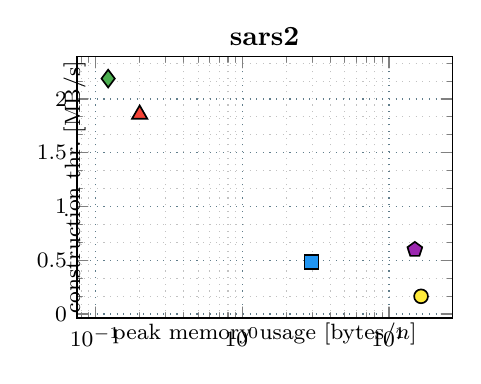
\begin{tikzpicture}[marks]
\begin{axis}[
    xmode=log,
    constructionstyle,
    title={sars2},
    ylabel={construction thr.\ [MB/s]},
    xlabel={peak memory usage [bytes/$n$]},
    y label style={at={(0.05,0.5)}},
]

%% MULTIPLOT(algo)
%% SELECT (peak_memory_usage / (1.0 * n)) AS x, ((n * 1000.0) / time_build) AS y, algo, text
%% FROM results_build
%% WHERE text='sars2.ACGT.50Gi'
%% GROUP BY algo
%% ORDER BY algo
\addplot[bmove] coordinates { (2.966,0.483012) };
\addlegendentry{algo=build\_bmove};
\addplot[brindex] coordinates { (16.53426,0.164354) };
\addlegendentry{algo=build\_br\_index};
\addplot[columba] coordinates { (15.0,0.598659) };
\addlegendentry{algo=build\_columba};
\addplot[moverb] coordinates { (0.12198,2.18972) };
\addlegendentry{algo=build\_move\_rb\_move};
\addplot[moverbrlzsa] coordinates { (0.2,1.85708) };
\addlegendentry{algo=build\_move\_rb\_rlzsa};

\legend{};
\end{axis}
\end{tikzpicture}
\end{subfigure}
\begin{subfigure}[h]{.31\textwidth}
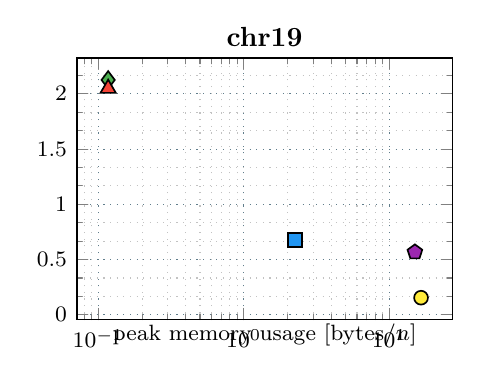
\begin{tikzpicture}[marks]
\begin{axis}[
    xmode=log,
    constructionstyle,
    title={chr19},
    xlabel={peak memory usage [bytes/$n$]},
    ylabel={\phantom{p}},
]

%% MULTIPLOT(algo)
%% SELECT (peak_memory_usage / (1.0 * n)) AS x, ((n * 1000.0) / time_build) AS y, algo, text
%% FROM results_build
%% WHERE text='chr19.ACGT.50Gi'
%% GROUP BY algo
%% ORDER BY algo
\addplot[bmove] coordinates { (2.252,0.677479) };
\addlegendentry{algo=build\_bmove};
\addplot[brindex] coordinates { (16.53076,0.154513) };
\addlegendentry{algo=build\_br\_index};
\addplot[columba] coordinates { (15.0,0.566893) };
\addlegendentry{algo=build\_columba};
\addplot[moverb] coordinates { (0.11696,2.1254) };
\addlegendentry{algo=build\_move\_rb\_move};
\addplot[moverbrlzsa] coordinates { (0.11696,2.04834) };
\addlegendentry{algo=build\_move\_rb\_rlzsa};

\legend{};
\end{axis}
\end{tikzpicture}
\end{subfigure}
\begin{subfigure}[h]{.31\textwidth}
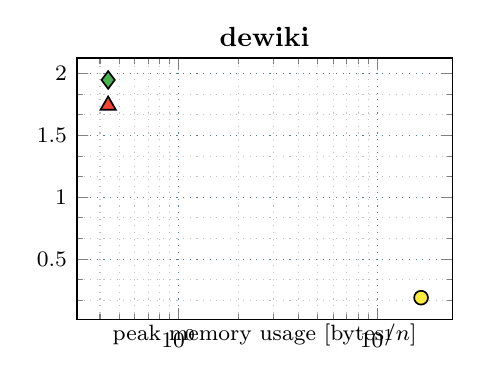
\begin{tikzpicture}[marks]
\begin{axis}[
    xmode=log,
    constructionstyle,
    title={dewiki},
    xlabel={peak memory usage [bytes/$n$]},
    ylabel={\phantom{p}},
]

%% MULTIPLOT(algo)
%% SELECT (peak_memory_usage / (1.0 * n)) AS x, ((n * 1000.0) / time_build) AS y, algo, text
%% FROM results_build
%% WHERE text='dewiki.50Gi'
%% GROUP BY algo
%% ORDER BY algo
\addplot[brindex] coordinates { (16.59768,0.187273) };
\addlegendentry{algo=build\_br\_index};
\addplot[moverb] coordinates { (0.44,1.94924) };
\addlegendentry{algo=build\_move\_rb\_move};
\addplot[moverbrlzsa] coordinates { (0.44,1.74368) };
\addlegendentry{algo=build\_move\_rb\_rlzsa};

\legend{};
\end{axis}
\end{tikzpicture}
\end{subfigure}

\vspace*{-0.35cm}

\centering
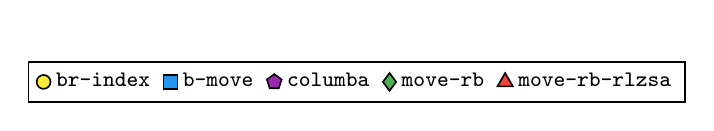
\begin{tikzpicture}[legendmarks]
\begin{axis}[legend,legend columns=5]
\addplot[brindex] coordinates { (0,0) };
\addlegendentry{\texttt{br-index}};
\addplot[bmove] coordinates { (0,0) };
\addlegendentry{\texttt{b-move}};
\addplot[columba] coordinates { (0,0) };
\addlegendentry{\texttt{columba}};
\addplot[moverb] coordinates { (0,0) };
\addlegendentry{\texttt{move-rb}};
\addplot[moverbrlzsa] coordinates { (0,0) };
\addlegendentry{\texttt{move-rb-rlzsa}};
\end{axis}
\end{tikzpicture}

\vspace*{-0.1cm}

\caption{\textup{[paper Figure 3.1 --- \texttt{charts/construction.tex}, from
\texttt{results-build.txt}]} Peak memory usage during index construction versus index
construction time.}
\label{fig:construction-memory-usage}
\end{figure*}

\begin{figure*}[t]
\centering
% IMPORT-DATA results_apm results/results-apm.txt

\begin{subfigure}[h]{.31\textwidth}
\hspace*{-0.4cm}
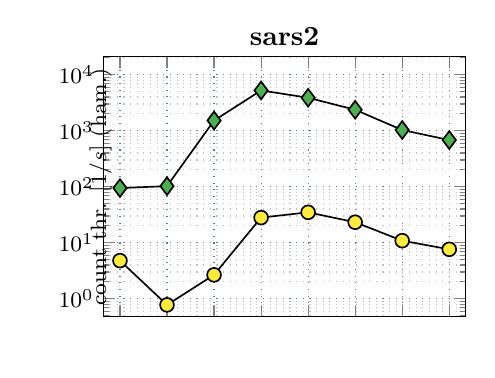
\begin{tikzpicture}[marks]
\begin{axis}[ymin=1e0,ymax=1e4,
    querystyle_apm,
    xticklabels={},
    title={sars2},
    ylabel={count thr. [$1/s$] (ham.)},
    y label style={at={(0.05,0.5)}},
    xmode=log,
    ymode=log,
    xlabel={\vphantom{pattern length}}
]

%% MULTIPLOT(algo)
%% SELECT pattern_length AS x, exp(avg(ln((num_patterns * pattern_length) / (time_count / 1000000000.0)))) AS y, algo
%% FROM results_apm
%% WHERE text = 'sars2.ACGT.50Gi' AND dist_metr = 'hamming' AND algo IN ('count_br_index_native', 'count_move_rb_move') AND cigar = 0
%% GROUP BY algo, pattern_length
%% ORDER BY algo, pattern_length
\addplot[brindex] coordinates { (10,4.78526) (20,0.774743) (40,2.66542) (80,28.0467) (160,34.8465) (320,23.1973) (640,10.8606) (1280,7.6142) };
\addlegendentry{algo=count\_br\_index\_native};
\addplot[moverb] coordinates { (10,94.4704) (20,102.286) (40,1516.64) (80,5233.77) (160,3875.03) (320,2364.14) (640,1028.44) (1280,680.715) };
\addlegendentry{algo=count\_move\_rb\_move};

\legend{};
\end{axis}
\end{tikzpicture}
\end{subfigure}
\begin{subfigure}[h]{.31\textwidth}
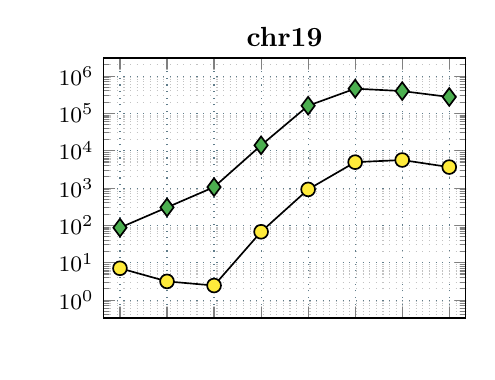
\begin{tikzpicture}[marks]
\begin{axis}[ymin=1e0,ymax=1e6,querystyle_apm,
    xticklabels={},
    title={chr19},
    ylabel={\phantom{p}},
    xmode=log,
    ymode=log,
    xlabel={\vphantom{pattern length}}
]

%% MULTIPLOT(algo)
%% SELECT pattern_length AS x, exp(avg(ln((num_patterns * pattern_length) / (time_count / 1000000000.0)))) AS y, algo
%% FROM results_apm
%% WHERE text = 'chr19.ACGT.50Gi' AND dist_metr = 'hamming' AND algo IN ('count_br_index_native', 'count_move_rb_move') AND cigar = 0
%% GROUP BY algo, pattern_length
%% ORDER BY algo, pattern_length
\addplot[brindex] coordinates { (10,7.10974) (20,3.1641) (40,2.4521) (80,67.521) (160,920.746) (320,4942.02) (640,5639.36) (1280,3648.79) };
\addlegendentry{algo=count\_br\_index\_native};
\addplot[moverb] coordinates { (10,86.7893) (20,303.283) (40,1062.78) (80,13976.2) (160,160543) (320,460172) (640,396108) (1280,275210) };
\addlegendentry{algo=count\_move\_rb\_move};

\legend{};
\end{axis}
\end{tikzpicture}
\end{subfigure}
\begin{subfigure}[h]{.31\textwidth}
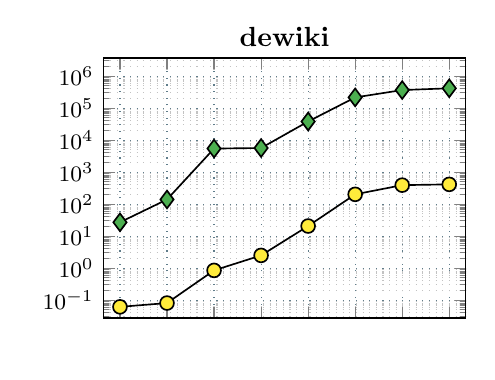
\begin{tikzpicture}[marks]
\begin{axis}[ymin=1e-1,ymax=1e6,querystyle_apm,
    xticklabels={},
    title={dewiki},
    ylabel={\phantom{p}},
    xmode=log,
    ymode=log,
    xlabel={\vphantom{pattern length}}
]

%% MULTIPLOT(algo)
%% SELECT pattern_length AS x, exp(avg(ln((num_patterns * pattern_length) / (time_count / 1000000000.0)))) AS y, algo
%% FROM results_apm
%% WHERE text = 'dewiki.50Gi' AND dist_metr = 'hamming' AND algo IN ('count_br_index_native', 'count_move_rb_move') AND cigar = 0
%% GROUP BY algo, pattern_length
%% ORDER BY algo, pattern_length
\addplot[brindex] coordinates { (10,0.0613695) (20,0.0806703) (40,0.846152) (80,2.48722) (160,20.5811) (320,201.331) (640,390.441) (1280,412.474) };
\addlegendentry{algo=count\_br\_index\_native};
\addplot[moverb] coordinates { (10,26.9207) (20,138.994) (40,5422.5) (80,5650.86) (160,37997.8) (320,215060) (640,365195) (1280,414752) };
\addlegendentry{algo=count\_move\_rb\_move};

\legend{};
\end{axis}
\end{tikzpicture}
\end{subfigure}

\vspace{-1.35cm}
\begin{subfigure}[h]{.31\textwidth}
\hspace*{-0.4cm}
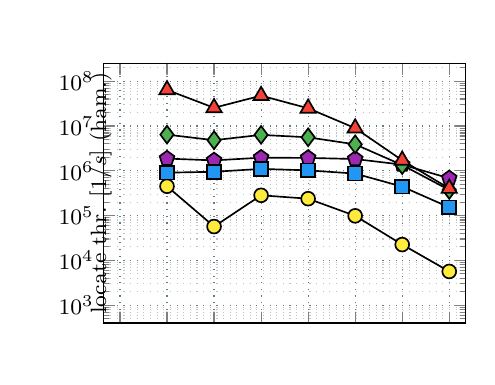
\begin{tikzpicture}[marks]
\begin{axis}[ymin=1e3,ymax=1e8,
    querystyle_apm,
    xticklabels={},
    ylabel={locate thr. [$1/s$] (ham.)},
    y label style={at={(0.05,0.5)}},
    xmode=log,
    ymode=log,
    title={\vphantom{Ig}},
    xlabel={\vphantom{pattern length}}
]

%% MULTIPLOT(algo)
%% SELECT pattern_length AS x, exp(avg(ln((num_patterns * pattern_length + (SELECT r.num_occurrences FROM results_apm r WHERE r.text = results_apm.text AND r.dist_metr = results_apm.dist_metr AND r.max_mismatches = results_apm.max_mismatches AND r.pattern_length = results_apm.pattern_length AND r.cigar = 0 AND r.algo = 'locate_move_rb_move')) / (time_locate / 1000000000.0)))) AS y, algo
%% FROM results_apm
%% WHERE text = 'sars2.ACGT.50Gi' AND dist_metr = 'hamming' AND algo IN ('locate_br_index_native', 'locate_columba', 'locate_columba_rlc', 'locate_move_rb_move', 'locate_move_rb_rlzsa') AND cigar = 0
%% GROUP BY algo, pattern_length
%% ORDER BY algo, pattern_length
\addplot[brindex] coordinates { (20,452389) (40,57031.8) (80,284056) (160,238553) (320,98866.8) (640,22586) (1280,5671.37) };
\addlegendentry{algo=locate\_br\_index\_native};
\addplot[columba] coordinates { (20,1.87585e+06) (40,1.70734e+06) (80,1.96437e+06) (160,1.94149e+06) (320,1.83237e+06) (640,1.37301e+06) (1280,681204) };
\addlegendentry{algo=locate\_columba};
\addplot[bmove] coordinates { (20,909400) (40,951979) (80,1.10325e+06) (160,1.024e+06) (320,867474) (640,444293) (1280,152998) };
\addlegendentry{algo=locate\_columba\_rlc};
\addplot[moverb] coordinates { (20,6.42541e+06) (40,4.8229e+06) (80,6.34363e+06) (160,5.59317e+06) (320,3.90036e+06) (640,1.34493e+06) (1280,374297) };
\addlegendentry{algo=locate\_move\_rb\_move};
\addplot[moverbrlzsa] coordinates { (20,6.39836e+07) (40,2.55151e+07) (80,4.76206e+07) (160,2.49084e+07) (320,8.97464e+06) (640,1.71732e+06) (1280,403913) };
\addlegendentry{algo=locate\_move\_rb\_rlzsa};

\legend{};
\end{axis}
\end{tikzpicture}
\end{subfigure}
\begin{subfigure}[h]{.31\textwidth}
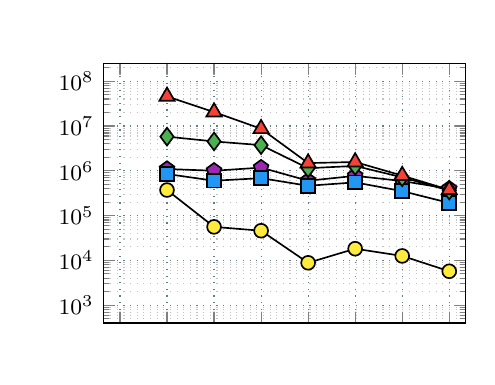
\begin{tikzpicture}[marks]
\begin{axis}[ymin=1e3,ymax=1e8,querystyle_apm,
    xticklabels={},
    ylabel={\phantom{p}},
    xmode=log,
    ymode=log,
    title={\vphantom{Ig}},
    xlabel={\vphantom{pattern length}}
]

%% MULTIPLOT(algo)
%% SELECT pattern_length AS x, exp(avg(ln((num_patterns * pattern_length + (SELECT r.num_occurrences FROM results_apm r WHERE r.text = results_apm.text AND r.dist_metr = results_apm.dist_metr AND r.max_mismatches = results_apm.max_mismatches AND r.pattern_length = results_apm.pattern_length AND r.cigar = 0 AND r.algo = 'locate_move_rb_move')) / (time_locate / 1000000000.0)))) AS y, algo
%% FROM results_apm
%% WHERE text = 'chr19.ACGT.50Gi' AND dist_metr = 'hamming' AND algo IN ('locate_br_index_native', 'locate_columba', 'locate_columba_rlc', 'locate_move_rb_move', 'locate_move_rb_rlzsa') AND cigar = 0
%% GROUP BY algo, pattern_length
%% ORDER BY algo, pattern_length
\addplot[brindex] coordinates { (20,372612) (40,56073.2) (80,45957.4) (160,8846.4) (320,18246.6) (640,12594.1) (1280,5729.2) };
\addlegendentry{algo=locate\_br\_index\_native};
\addplot[columba] coordinates { (20,1.09834e+06) (40,1.00289e+06) (80,1.17828e+06) (160,601061) (320,771606) (640,592002) (1280,397340) };
\addlegendentry{algo=locate\_columba};
\addplot[bmove] coordinates { (20,848885) (40,600551) (80,685872) (160,463447) (320,552001) (640,352228) (1280,192018) };
\addlegendentry{algo=locate\_columba\_rlc};
\addplot[moverb] coordinates { (20,5.79088e+06) (40,4.52647e+06) (80,3.74344e+06) (160,1.14393e+06) (320,1.28509e+06) (640,716054) (1280,363177) };
\addlegendentry{algo=locate\_move\_rb\_move};
\addplot[moverbrlzsa] coordinates { (20,4.58147e+07) (40,2.04906e+07) (80,8.69383e+06) (160,1.48744e+06) (320,1.57242e+06) (640,782034) (1280,375528) };
\addlegendentry{algo=locate\_move\_rb\_rlzsa};

\legend{};
\end{axis}
\end{tikzpicture}
\end{subfigure}
\begin{subfigure}[h]{.31\textwidth}
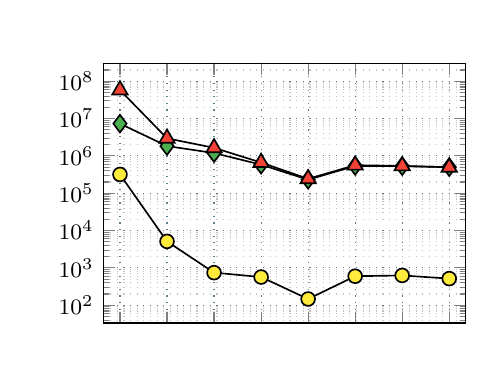
\begin{tikzpicture}[marks]
\begin{axis}[ymin=1e2,ymax=1e8,querystyle_apm,
    xticklabels={},
    ylabel={\phantom{p}},
    xmode=log,
    ymode=log,
    title={\vphantom{Ig}},
    xlabel={\vphantom{pattern length}}
]

%% MULTIPLOT(algo)
%% SELECT pattern_length AS x, exp(avg(ln((num_patterns * pattern_length + (SELECT r.num_occurrences FROM results_apm r WHERE r.text = results_apm.text AND r.dist_metr = results_apm.dist_metr AND r.max_mismatches = results_apm.max_mismatches AND r.pattern_length = results_apm.pattern_length AND r.cigar = 0 AND r.algo = 'locate_move_rb_move')) / (time_locate / 1000000000.0)))) AS y, algo
%% FROM results_apm
%% WHERE text = 'dewiki.50Gi' AND dist_metr = 'hamming' AND algo IN ('locate_br_index_native', 'locate_columba', 'locate_columba_rlc', 'locate_move_rb_move', 'locate_move_rb_rlzsa') AND cigar = 0
%% GROUP BY algo, pattern_length
%% ORDER BY algo, pattern_length
\addplot[brindex] coordinates { (10,318378) (20,5118.52) (40,745.944) (80,568.671) (160,146.804) (320,598.418) (640,627.528) (1280,516.473) };
\addlegendentry{algo=locate\_br\_index\_native};
\addplot[moverb] coordinates { (10,7.31258e+06) (20,1.8323e+06) (40,1.19248e+06) (80,581436) (160,230011) (320,538879) (640,529707) (1280,499884) };
\addlegendentry{algo=locate\_move\_rb\_move};
\addplot[moverbrlzsa] coordinates { (10,5.81153e+07) (20,2.95186e+06) (40,1.64334e+06) (80,663769) (160,242821) (320,562836) (640,538545) (1280,495446) };
\addlegendentry{algo=locate\_move\_rb\_rlzsa};

\legend{};
\end{axis}
\end{tikzpicture}
\end{subfigure}

\vspace{-1.35cm}
\begin{subfigure}[h]{.31\textwidth}
\hspace*{-0.4cm}
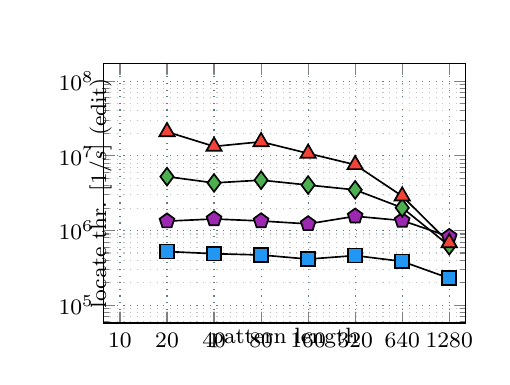
\begin{tikzpicture}[marks]
\begin{axis}[ymin=1e5,ymax=1e8,
    querystyle_apm,
    xlabel={pattern length},
    ylabel={locate thr. [$1/s$] (edit)},
    y label style={at={(0.05,0.5)}},
    xmode=log,
    ymode=log,,
    title={\vphantom{Ig}}
]

%% MULTIPLOT(algo)
%% SELECT pattern_length AS x, exp(avg(ln((num_patterns * pattern_length + (SELECT r.num_occurrences FROM results_apm r WHERE r.text = results_apm.text AND r.dist_metr = results_apm.dist_metr AND r.max_mismatches = results_apm.max_mismatches AND r.pattern_length = results_apm.pattern_length AND r.cigar = 0 AND r.algo = 'locate_move_rb_move')) / (time_locate / 1000000000.0)))) AS y, algo
%% FROM results_apm
%% WHERE text = 'sars2.ACGT.50Gi' AND dist_metr = 'edit' AND algo IN ('locate_columba', 'locate_columba_rlc', 'locate_move_rb_move', 'locate_move_rb_rlzsa') AND cigar = 0
%% GROUP BY algo, pattern_length
%% ORDER BY algo, pattern_length
\addplot[columba] coordinates { (20,1.33696e+06) (40,1.42917e+06) (80,1.34394e+06) (160,1.22813e+06) (320,1.55483e+06) (640,1.36112e+06) (1280,828384) };
\addlegendentry{algo=locate\_columba};
\addplot[bmove] coordinates { (20,523839) (40,489525) (80,470758) (160,414654) (320,462121) (640,386244) (1280,229694) };
\addlegendentry{algo=locate\_columba\_rlc};
\addplot[moverb] coordinates { (20,5.27563e+06) (40,4.34548e+06) (80,4.732e+06) (160,4.06949e+06) (320,3.50736e+06) (640,2.01783e+06) (1280,625990) };
\addlegendentry{algo=locate\_move\_rb\_move};
\addplot[moverbrlzsa] coordinates { (20,2.09949e+07) (40,1.33959e+07) (80,1.54486e+07) (160,1.0804e+07) (320,7.61368e+06) (640,2.88973e+06) (1280,686311) };
\addlegendentry{algo=locate\_move\_rb\_rlzsa};

\legend{};
\end{axis}
\end{tikzpicture}
\end{subfigure}
\begin{subfigure}[h]{.31\textwidth}
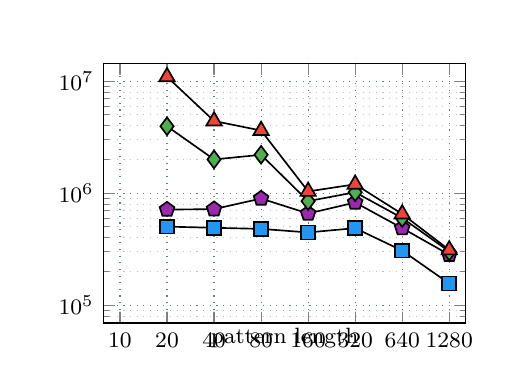
\begin{tikzpicture}[marks]
\begin{axis}[ymin=1e5,ymax=1e7,querystyle_apm,
    xlabel={pattern length},
    ylabel={\phantom{p}},
    xmode=log,
    ymode=log,,
    title={\vphantom{Ig}}
]

%% MULTIPLOT(algo)
%% SELECT pattern_length AS x, exp(avg(ln((num_patterns * pattern_length + (SELECT r.num_occurrences FROM results_apm r WHERE r.text = results_apm.text AND r.dist_metr = results_apm.dist_metr AND r.max_mismatches = results_apm.max_mismatches AND r.pattern_length = results_apm.pattern_length AND r.cigar = 0 AND r.algo = 'locate_move_rb_move')) / (time_locate / 1000000000.0)))) AS y, algo
%% FROM results_apm
%% WHERE text = 'chr19.ACGT.50Gi' AND dist_metr = 'edit' AND algo IN ('locate_columba', 'locate_columba_rlc', 'locate_move_rb_move', 'locate_move_rb_rlzsa') AND cigar = 0
%% GROUP BY algo, pattern_length
%% ORDER BY algo, pattern_length
\addplot[columba] coordinates { (20,714669) (40,720644) (80,896454) (160,658656) (320,825919) (640,487781) (1280,282250) };
\addlegendentry{algo=locate\_columba};
\addplot[bmove] coordinates { (20,503202) (40,491082) (80,480209) (160,446471) (320,487548) (640,307223) (1280,156122) };
\addlegendentry{algo=locate\_columba\_rlc};
\addplot[moverb] coordinates { (20,3.96068e+06) (40,2.00234e+06) (80,2.20246e+06) (160,849777) (320,1.01968e+06) (640,600377) (1280,301809) };
\addlegendentry{algo=locate\_move\_rb\_move};
\addplot[moverbrlzsa] coordinates { (20,1.09534e+07) (40,4.41251e+06) (80,3.62966e+06) (160,1.03771e+06) (320,1.20102e+06) (640,652162) (1280,311544) };
\addlegendentry{algo=locate\_move\_rb\_rlzsa};

\legend{};
\end{axis}
\end{tikzpicture}
\end{subfigure}
\begin{subfigure}[h]{.31\textwidth}
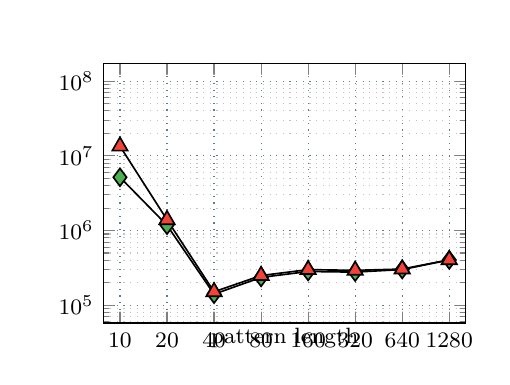
\begin{tikzpicture}[marks]
\begin{axis}[ymin=1e5,ymax=1e8,querystyle_apm,
    xlabel={pattern length},
    ylabel={\phantom{p}},
    xmode=log,
    ymode=log,,
    title={\vphantom{Ig}}
]

%% MULTIPLOT(algo)
%% SELECT pattern_length AS x, exp(avg(ln((num_patterns * pattern_length + (SELECT r.num_occurrences FROM results_apm r WHERE r.text = results_apm.text AND r.dist_metr = results_apm.dist_metr AND r.max_mismatches = results_apm.max_mismatches AND r.pattern_length = results_apm.pattern_length AND r.cigar = 0 AND r.algo = 'locate_move_rb_move')) / (time_locate / 1000000000.0)))) AS y, algo
%% FROM results_apm
%% WHERE text = 'dewiki.50Gi' AND dist_metr = 'edit' AND algo IN ('locate_columba', 'locate_columba_rlc', 'locate_move_rb_move', 'locate_move_rb_rlzsa') AND cigar = 0
%% GROUP BY algo, pattern_length
%% ORDER BY algo, pattern_length
\addplot[moverb] coordinates { (10,5.16966e+06) (20,1.17815e+06) (40,140602) (80,235716) (160,282849) (320,277565) (640,300730) (1280,403425) };
\addlegendentry{algo=locate\_move\_rb\_move};
\addplot[moverbrlzsa] coordinates { (10,1.34878e+07) (20,1.39526e+06) (40,151395) (80,249623) (160,299757) (320,293016) (640,305030) (1280,406089) };
\addlegendentry{algo=locate\_move\_rb\_rlzsa};

\legend{};
\end{axis}
\end{tikzpicture}
\end{subfigure}

\vspace*{-0.35cm}

\centering
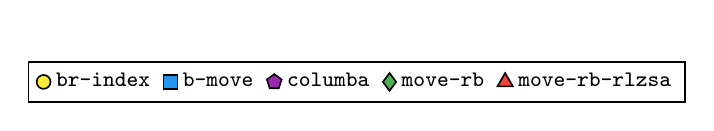
\begin{tikzpicture}[legendmarks]
\begin{axis}[legend,legend columns=5]
\addplot[brindex] coordinates { (0,0) };
\addlegendentry{\texttt{br-index}};
\addplot[bmove] coordinates { (0,0) };
\addlegendentry{\texttt{b-move}};
\addplot[columba] coordinates { (0,0) };
\addlegendentry{\texttt{columba}};
\addplot[moverb] coordinates { (0,0) };
\addlegendentry{\texttt{move-rb}};
\addplot[moverbrlzsa] coordinates { (0,0) };
\addlegendentry{\texttt{move-rb-rlzsa}};
\end{axis}
\end{tikzpicture}

\vspace*{-0.1cm}

\caption{\textup{[paper Figure 3.2 --- \texttt{charts/apm.tex}, from
\texttt{results-apm.txt}]} APM query throughput as a geometric mean over the results for
$k \in \{4, 7, 10, 13\}$. All indexes use their native APM algorithms.}
\label{fig:apm}
\end{figure*}

% paper Table C.1 -- brings its own table* environment and caption
% IMPORT-DATA results_apm results/results-apm.txt

\begin{table*}[t!]
\centering
\scriptsize
\setlength{\tabcolsep}{2.1pt}
\renewcommand{\arraystretch}{1.0}
\begin{tabular}{|rr|rrr|rr|rrr|rr|rrr||rr|r|rr|r|r|}
\hline
\multicolumn{2}{|c|}{} & \multicolumn{13}{c||}{hamming distance} & \multicolumn{7}{c|}{edit distance} \\
\cline{3-15}\cline{16-22}
\multicolumn{2}{|c|}{} & \multicolumn{5}{c|}{sars2} & \multicolumn{5}{c|}{chr19} & \multicolumn{3}{c||}{dewiki} & \multicolumn{3}{c|}{sars2} & \multicolumn{3}{c|}{chr19} & \multicolumn{1}{c|}{dewiki} \\
\hline
$k$ & $m$ & $\frac{\pk{\iM}}{\isz{\iM}}$ & $\frac{\pk{\iB}}{\isz{\iB}}$ & $\frac{\pks{\iR}}{\isz{\iR}}$ & $\frac{\pk{\iB}}{\pk{\iM}}$ & $\frac{\pks{\iR}}{\pks{\iM}}$ & $\frac{\pk{\iM}}{\isz{\iM}}$ & $\frac{\pk{\iB}}{\isz{\iB}}$ & $\frac{\pks{\iR}}{\isz{\iR}}$ & $\frac{\pk{\iB}}{\pk{\iM}}$ & $\frac{\pks{\iR}}{\pks{\iM}}$ & $\frac{\pk{\iM}}{\isz{\iM}}$ & $\frac{\pks{\iR}}{\isz{\iR}}$ & $\frac{\pks{\iR}}{\pks{\iM}}$ & $\frac{\pk{\iM}}{\isz{\iM}}$ & $\frac{\pk{\iB}}{\isz{\iB}}$ & $\frac{\pk{\iB}}{\pk{\iM}}$ & $\frac{\pk{\iM}}{\isz{\iM}}$ & $\frac{\pk{\iB}}{\isz{\iB}}$ & $\frac{\pk{\iB}}{\pk{\iM}}$ & $\frac{\pk{\iM}}{\isz{\iM}}$ \\
\hline
%% TABULAR
%% WITH ms AS (SELECT DISTINCT max_mismatches AS k, pattern_length AS m FROM results_apm WHERE algo = 'locate_move_rb_move' AND dist_metr IN ('hamming','edit') AND cigar = 1),
%% hsm1 AS (SELECT max_mismatches AS k, pattern_length AS m, index_mem AS ix, index_mem + peak_mem AS pk FROM results_apm WHERE text = 'sars2.ACGT.50Gi' AND algo = 'locate_move_rb_move' AND dist_metr = 'hamming' AND cigar = 1),
%% hsb1 AS (SELECT max_mismatches AS k, pattern_length AS m, index_mem AS ix, index_mem + peak_mem AS pk FROM results_apm WHERE text = 'sars2.ACGT.50Gi' AND algo = 'locate_columba_rlc' AND dist_metr = 'hamming' AND cigar = 1),
%% hsr0 AS (SELECT max_mismatches AS k, pattern_length AS m, index_mem AS ix, index_mem + peak_mem AS pk FROM results_apm WHERE text = 'sars2.ACGT.50Gi' AND algo = 'locate_br_index' AND dist_metr = 'hamming' AND cigar = 0),
%% hsm0 AS (SELECT max_mismatches AS k, pattern_length AS m, index_mem AS ix, index_mem + peak_mem AS pk FROM results_apm WHERE text = 'sars2.ACGT.50Gi' AND algo = 'locate_move_rb_move' AND dist_metr = 'hamming' AND cigar = 0),
%% hcm1 AS (SELECT max_mismatches AS k, pattern_length AS m, index_mem AS ix, index_mem + peak_mem AS pk FROM results_apm WHERE text = 'chr19.ACGT.50Gi' AND algo = 'locate_move_rb_move' AND dist_metr = 'hamming' AND cigar = 1),
%% hcb1 AS (SELECT max_mismatches AS k, pattern_length AS m, index_mem AS ix, index_mem + peak_mem AS pk FROM results_apm WHERE text = 'chr19.ACGT.50Gi' AND algo = 'locate_columba_rlc' AND dist_metr = 'hamming' AND cigar = 1),
%% hcr0 AS (SELECT max_mismatches AS k, pattern_length AS m, index_mem AS ix, index_mem + peak_mem AS pk FROM results_apm WHERE text = 'chr19.ACGT.50Gi' AND algo = 'locate_br_index' AND dist_metr = 'hamming' AND cigar = 0),
%% hcm0 AS (SELECT max_mismatches AS k, pattern_length AS m, index_mem AS ix, index_mem + peak_mem AS pk FROM results_apm WHERE text = 'chr19.ACGT.50Gi' AND algo = 'locate_move_rb_move' AND dist_metr = 'hamming' AND cigar = 0),
%% hdm1 AS (SELECT max_mismatches AS k, pattern_length AS m, index_mem AS ix, index_mem + peak_mem AS pk FROM results_apm WHERE text = 'dewiki.50Gi' AND algo = 'locate_move_rb_move' AND dist_metr = 'hamming' AND cigar = 1),
%% hdr0 AS (SELECT max_mismatches AS k, pattern_length AS m, index_mem AS ix, index_mem + peak_mem AS pk FROM results_apm WHERE text = 'dewiki.50Gi' AND algo = 'locate_br_index' AND dist_metr = 'hamming' AND cigar = 0),
%% hdm0 AS (SELECT max_mismatches AS k, pattern_length AS m, index_mem AS ix, index_mem + peak_mem AS pk FROM results_apm WHERE text = 'dewiki.50Gi' AND algo = 'locate_move_rb_move' AND dist_metr = 'hamming' AND cigar = 0),
%% esm1 AS (SELECT max_mismatches AS k, pattern_length AS m, index_mem AS ix, index_mem + peak_mem AS pk FROM results_apm WHERE text = 'sars2.ACGT.50Gi' AND algo = 'locate_move_rb_move' AND dist_metr = 'edit' AND cigar = 1),
%% esb1 AS (SELECT max_mismatches AS k, pattern_length AS m, index_mem AS ix, index_mem + peak_mem AS pk FROM results_apm WHERE text = 'sars2.ACGT.50Gi' AND algo = 'locate_columba_rlc' AND dist_metr = 'edit' AND cigar = 1),
%% ecm1 AS (SELECT max_mismatches AS k, pattern_length AS m, index_mem AS ix, index_mem + peak_mem AS pk FROM results_apm WHERE text = 'chr19.ACGT.50Gi' AND algo = 'locate_move_rb_move' AND dist_metr = 'edit' AND cigar = 1),
%% ecb1 AS (SELECT max_mismatches AS k, pattern_length AS m, index_mem AS ix, index_mem + peak_mem AS pk FROM results_apm WHERE text = 'chr19.ACGT.50Gi' AND algo = 'locate_columba_rlc' AND dist_metr = 'edit' AND cigar = 1),
%% edm1 AS (SELECT max_mismatches AS k, pattern_length AS m, index_mem AS ix, index_mem + peak_mem AS pk FROM results_apm WHERE text = 'dewiki.50Gi' AND algo = 'locate_move_rb_move' AND dist_metr = 'edit' AND cigar = 1)
%% SELECT printf('\num{%d}', ms.k), printf('\num{%d}', ms.m),
%%   CASE WHEN hsm1.pk IS NULL THEN '' ELSE printf('\num{%.2f}', 1.0 * hsm1.pk / hsm1.ix) END,
%%   CASE WHEN hsb1.pk IS NULL THEN '' WHEN 1.0 * hsb1.pk / hsb1.ix >= 1.2 THEN printf('\textbf{%.2f}', 1.0 * hsb1.pk / hsb1.ix) ELSE printf('\num{%.2f}', 1.0 * hsb1.pk / hsb1.ix) END,
%%   CASE WHEN hsr0.pk IS NULL THEN '' WHEN 1.0 * hsr0.pk / hsr0.ix >= 1.2 THEN printf('\textbf{%.2f}', 1.0 * hsr0.pk / hsr0.ix) ELSE printf('\num{%.2f}', 1.0 * hsr0.pk / hsr0.ix) END,
%%   CASE WHEN hsb1.pk IS NULL OR hsm1.pk IS NULL THEN '' WHEN 1.0 * hsb1.pk / hsm1.pk >= 1.2 THEN printf('\textbf{%.2f}', 1.0 * hsb1.pk / hsm1.pk) ELSE printf('\num{%.2f}', 1.0 * hsb1.pk / hsm1.pk) END,
%%   CASE WHEN hsr0.pk IS NULL OR hsm0.pk IS NULL THEN '' ELSE printf('\num{%.2f}', 1.0 * hsr0.pk / hsm0.pk) END,
%%   CASE WHEN hcm1.pk IS NULL THEN '' ELSE printf('\num{%.2f}', 1.0 * hcm1.pk / hcm1.ix) END,
%%   CASE WHEN hcb1.pk IS NULL THEN '' WHEN 1.0 * hcb1.pk / hcb1.ix >= 1.2 THEN printf('\textbf{%.2f}', 1.0 * hcb1.pk / hcb1.ix) ELSE printf('\num{%.2f}', 1.0 * hcb1.pk / hcb1.ix) END,
%%   CASE WHEN hcr0.pk IS NULL THEN '' WHEN 1.0 * hcr0.pk / hcr0.ix >= 1.2 THEN printf('\textbf{%.2f}', 1.0 * hcr0.pk / hcr0.ix) ELSE printf('\num{%.2f}', 1.0 * hcr0.pk / hcr0.ix) END,
%%   CASE WHEN hcb1.pk IS NULL OR hcm1.pk IS NULL THEN '' WHEN 1.0 * hcb1.pk / hcm1.pk >= 1.2 THEN printf('\textbf{%.2f}', 1.0 * hcb1.pk / hcm1.pk) ELSE printf('\num{%.2f}', 1.0 * hcb1.pk / hcm1.pk) END,
%%   CASE WHEN hcr0.pk IS NULL OR hcm0.pk IS NULL THEN '' ELSE printf('\num{%.2f}', 1.0 * hcr0.pk / hcm0.pk) END,
%%   CASE WHEN hdm1.pk IS NULL THEN '' ELSE printf('\num{%.2f}', 1.0 * hdm1.pk / hdm1.ix) END,
%%   CASE WHEN hdr0.pk IS NULL THEN '' WHEN 1.0 * hdr0.pk / hdr0.ix >= 1.2 THEN printf('\textbf{%.2f}', 1.0 * hdr0.pk / hdr0.ix) ELSE printf('\num{%.2f}', 1.0 * hdr0.pk / hdr0.ix) END,
%%   CASE WHEN hdr0.pk IS NULL OR hdm0.pk IS NULL THEN '' ELSE printf('\num{%.2f}', 1.0 * hdr0.pk / hdm0.pk) END,
%%   CASE WHEN esm1.pk IS NULL THEN '' ELSE printf('\num{%.2f}', 1.0 * esm1.pk / esm1.ix) END,
%%   CASE WHEN esb1.pk IS NULL THEN '' WHEN 1.0 * esb1.pk / esb1.ix >= 1.2 THEN printf('\textbf{%.2f}', 1.0 * esb1.pk / esb1.ix) ELSE printf('\num{%.2f}', 1.0 * esb1.pk / esb1.ix) END,
%%   CASE WHEN esb1.pk IS NULL OR esm1.pk IS NULL THEN '' WHEN 1.0 * esb1.pk / esm1.pk >= 1.2 THEN printf('\textbf{%.2f}', 1.0 * esb1.pk / esm1.pk) ELSE printf('\num{%.2f}', 1.0 * esb1.pk / esm1.pk) END,
%%   CASE WHEN ecm1.pk IS NULL THEN '' ELSE printf('\num{%.2f}', 1.0 * ecm1.pk / ecm1.ix) END,
%%   CASE WHEN ecb1.pk IS NULL THEN '' WHEN 1.0 * ecb1.pk / ecb1.ix >= 1.2 THEN printf('\textbf{%.2f}', 1.0 * ecb1.pk / ecb1.ix) ELSE printf('\num{%.2f}', 1.0 * ecb1.pk / ecb1.ix) END,
%%   CASE WHEN ecb1.pk IS NULL OR ecm1.pk IS NULL THEN '' WHEN 1.0 * ecb1.pk / ecm1.pk >= 1.2 THEN printf('\textbf{%.2f}', 1.0 * ecb1.pk / ecm1.pk) ELSE printf('\num{%.2f}', 1.0 * ecb1.pk / ecm1.pk) END,
%%   CASE WHEN edm1.pk IS NULL THEN '' ELSE printf('\num{%.2f}', 1.0 * edm1.pk / edm1.ix) END
%% FROM ms LEFT JOIN hsm1 ON hsm1.k = ms.k AND hsm1.m = ms.m LEFT JOIN hsb1 ON hsb1.k = ms.k AND hsb1.m = ms.m LEFT JOIN hsr0 ON hsr0.k = ms.k AND hsr0.m = ms.m LEFT JOIN hsm0 ON hsm0.k = ms.k AND hsm0.m = ms.m LEFT JOIN hcm1 ON hcm1.k = ms.k AND hcm1.m = ms.m LEFT JOIN hcb1 ON hcb1.k = ms.k AND hcb1.m = ms.m LEFT JOIN hcr0 ON hcr0.k = ms.k AND hcr0.m = ms.m LEFT JOIN hcm0 ON hcm0.k = ms.k AND hcm0.m = ms.m LEFT JOIN hdm1 ON hdm1.k = ms.k AND hdm1.m = ms.m LEFT JOIN hdr0 ON hdr0.k = ms.k AND hdr0.m = ms.m LEFT JOIN hdm0 ON hdm0.k = ms.k AND hdm0.m = ms.m LEFT JOIN esm1 ON esm1.k = ms.k AND esm1.m = ms.m LEFT JOIN esb1 ON esb1.k = ms.k AND esb1.m = ms.m LEFT JOIN ecm1 ON ecm1.k = ms.k AND ecm1.m = ms.m LEFT JOIN ecb1 ON ecb1.k = ms.k AND ecb1.m = ms.m LEFT JOIN edm1 ON edm1.k = ms.k AND edm1.m = ms.m ORDER BY ms.k, ms.m
 \num{4} &   \num{10} &            &               &               &               &            &            &               &               &               &            & \num{1.04} & \num{1.04} & \num{0.48} &            &               &               &            &               &               & \num{1.04} \\
 \num{4} &   \num{20} & \num{1.03} & \textbf{1.37} &    \num{1.04} & \textbf{1.33} & \num{0.48} & \num{1.24} & \textbf{3.61} & \textbf{1.25} & \textbf{3.80} & \num{0.55} & \num{1.02} & \num{1.03} & \num{0.48} & \num{1.10} & \textbf{1.99} & \textbf{1.80} & \num{1.97} & \textbf{7.93} & \textbf{5.26} & \num{1.02} \\
 \num{4} &   \num{40} & \num{1.01} &    \num{1.19} &    \num{1.03} &    \num{1.17} & \num{0.47} & \num{1.12} & \textbf{1.65} &    \num{1.13} & \textbf{1.93} & \num{0.52} & \num{1.00} & \num{1.01} & \num{0.48} & \num{1.10} & \textbf{2.04} & \textbf{1.85} & \num{1.24} & \textbf{2.90} & \textbf{3.06} & \num{1.00} \\
 \num{4} &   \num{80} & \num{1.01} &    \num{1.19} &    \num{1.02} &    \num{1.17} & \num{0.47} & \num{1.01} &    \num{1.08} &    \num{1.01} & \textbf{1.41} & \num{0.49} & \num{1.00} & \num{1.00} & \num{0.47} & \num{1.10} & \textbf{2.16} & \textbf{1.96} & \num{1.02} &    \num{1.13} & \textbf{1.46} & \num{1.00} \\
 \num{4} &  \num{160} & \num{1.01} &    \num{1.19} &    \num{1.02} &    \num{1.17} & \num{0.47} & \num{1.00} &    \num{1.00} &    \num{1.00} & \textbf{1.31} & \num{0.49} & \num{1.00} & \num{1.00} & \num{0.47} & \num{1.05} & \textbf{2.38} & \textbf{2.26} & \num{1.00} &    \num{1.01} & \textbf{1.32} & \num{1.00} \\
 \num{4} &  \num{320} & \num{1.01} &    \num{1.18} &    \num{1.02} &    \num{1.17} & \num{0.47} & \num{1.00} &    \num{1.00} &    \num{1.00} & \textbf{1.31} & \num{0.49} & \num{1.00} & \num{1.00} & \num{0.47} & \num{1.05} & \textbf{2.77} & \textbf{2.63} & \num{1.00} &    \num{1.00} & \textbf{1.31} & \num{1.00} \\
 \num{4} &  \num{640} & \num{1.01} &    \num{1.10} &    \num{1.02} &    \num{1.08} & \num{0.47} & \num{1.00} &    \num{1.00} &    \num{1.00} & \textbf{1.31} & \num{0.49} & \num{1.00} & \num{1.00} & \num{0.47} & \num{1.05} & \textbf{3.57} & \textbf{3.39} & \num{1.00} &    \num{1.00} & \textbf{1.31} & \num{1.00} \\
 \num{4} & \num{1280} & \num{1.01} &    \num{1.19} &    \num{1.02} &    \num{1.17} & \num{0.47} & \num{1.00} &    \num{1.00} &    \num{1.00} & \textbf{1.31} & \num{0.49} & \num{1.00} & \num{1.00} & \num{0.47} & \num{1.05} & \textbf{3.20} & \textbf{3.03} & \num{1.00} &    \num{1.00} & \textbf{1.31} & \num{1.00} \\
 \num{7} &   \num{20} & \num{1.21} & \textbf{3.93} & \textbf{1.23} & \textbf{3.25} & \num{0.52} & \num{1.24} & \textbf{3.61} & \textbf{1.25} & \textbf{3.80} & \num{0.55} & \num{1.00} & \num{1.00} & \num{0.48} &            &               &               &            &               &               & \num{1.00} \\
 \num{7} &   \num{40} & \num{1.01} &    \num{1.19} &    \num{1.02} &    \num{1.17} & \num{0.47} & \num{1.12} & \textbf{2.31} &    \num{1.13} & \textbf{2.69} & \num{0.52} & \num{1.00} & \num{1.01} & \num{0.48} & \num{1.11} & \textbf{2.91} & \textbf{2.63} & \num{1.50} & \textbf{6.95} & \textbf{6.07} & \num{1.00} \\
 \num{7} &   \num{80} & \num{1.01} &    \num{1.19} &    \num{1.02} &    \num{1.17} & \num{0.47} & \num{1.03} &    \num{1.16} &    \num{1.03} & \textbf{1.48} & \num{0.50} & \num{1.00} & \num{1.00} & \num{0.48} & \num{1.10} & \textbf{2.97} & \textbf{2.69} & \num{1.06} & \textbf{1.93} & \textbf{2.38} & \num{1.00} \\
 \num{7} &  \num{160} & \num{1.01} &    \num{1.19} &    \num{1.02} &    \num{1.17} & \num{0.47} & \num{1.00} &    \num{1.01} &    \num{1.00} & \textbf{1.32} & \num{0.49} & \num{1.00} & \num{1.00} & \num{0.47} & \num{1.11} & \textbf{3.49} & \textbf{3.15} & \num{1.00} &    \num{1.02} & \textbf{1.33} & \num{1.00} \\
 \num{7} &  \num{320} & \num{1.01} &    \num{1.18} &    \num{1.02} &    \num{1.17} & \num{0.47} & \num{1.00} &    \num{1.00} &    \num{1.00} & \textbf{1.31} & \num{0.49} & \num{1.00} & \num{1.00} & \num{0.47} & \num{1.11} & \textbf{4.07} & \textbf{3.68} & \num{1.00} &    \num{1.00} & \textbf{1.31} & \num{1.00} \\
 \num{7} &  \num{640} & \num{1.01} &    \num{1.19} &    \num{1.02} &    \num{1.17} & \num{0.47} & \num{1.00} &    \num{1.00} &    \num{1.00} & \textbf{1.31} & \num{0.49} & \num{1.00} & \num{1.00} & \num{0.47} & \num{1.11} & \textbf{5.24} & \textbf{4.73} & \num{1.00} &    \num{1.00} & \textbf{1.31} & \num{1.00} \\
 \num{7} & \num{1280} & \num{1.01} &    \num{1.10} &    \num{1.02} &    \num{1.08} & \num{0.47} & \num{1.00} &    \num{1.00} &    \num{1.00} & \textbf{1.31} & \num{0.49} & \num{1.00} & \num{1.00} & \num{0.47} & \num{1.11} & \textbf{5.33} & \textbf{4.78} & \num{1.00} &    \num{1.00} & \textbf{1.31} & \num{1.00} \\
\num{10} &   \num{20} &            &               &               &               &            &            &               &               &               &            & \num{1.00} & \num{1.00} & \num{0.48} &            &               &               &            &               &               &            \\
\num{10} &   \num{40} & \num{1.01} & \textbf{1.37} &    \num{1.02} & \textbf{1.35} & \num{0.47} & \num{1.12} & \textbf{3.61} &    \num{1.13} & \textbf{4.21} & \num{0.52} & \num{1.00} & \num{1.00} & \num{0.48} & \num{1.21} & \textbf{4.56} & \textbf{3.76} & \num{1.07} & \textbf{1.72} & \textbf{2.11} & \num{1.00} \\
\num{10} &   \num{80} & \num{1.01} & \textbf{1.37} &    \num{1.02} & \textbf{1.35} & \num{0.47} & \num{1.06} & \textbf{1.65} &    \num{1.06} & \textbf{2.04} & \num{0.51} & \num{1.01} & \num{1.01} & \num{0.48} & \num{1.21} & \textbf{4.92} & \textbf{4.06} & \num{1.25} & \textbf{2.55} & \textbf{2.66} & \num{1.00} \\
\num{10} &  \num{160} & \num{1.01} & \textbf{1.37} &    \num{1.02} & \textbf{1.35} & \num{0.47} & \num{1.00} &    \num{1.01} &    \num{1.00} & \textbf{1.32} & \num{0.49} & \num{1.00} & \num{1.00} & \num{0.47} & \num{1.11} & \textbf{3.47} & \textbf{3.14} & \num{1.01} &    \num{1.11} & \textbf{1.44} & \num{1.00} \\
\num{10} &  \num{320} & \num{1.01} &    \num{1.19} &    \num{1.02} &    \num{1.17} & \num{0.47} & \num{1.00} &    \num{1.00} &    \num{1.00} & \textbf{1.31} & \num{0.49} & \num{1.00} & \num{1.00} & \num{0.47} & \num{1.21} & \textbf{6.71} & \textbf{5.54} & \num{1.00} &    \num{1.00} & \textbf{1.32} & \num{1.00} \\
\num{10} &  \num{640} & \num{1.01} & \textbf{1.37} &    \num{1.02} & \textbf{1.35} & \num{0.47} & \num{1.00} &    \num{1.00} &    \num{1.00} & \textbf{1.31} & \num{0.49} & \num{1.00} & \num{1.00} & \num{0.47} & \num{1.11} & \textbf{8.24} & \textbf{7.42} & \num{1.00} &    \num{1.00} & \textbf{1.32} & \num{1.00} \\
\num{10} & \num{1280} & \num{1.01} & \textbf{1.21} &    \num{1.02} &    \num{1.19} & \num{0.47} & \num{1.00} &    \num{1.00} &    \num{1.00} & \textbf{1.31} & \num{0.49} & \num{1.00} & \num{1.00} & \num{0.47} & \num{1.06} & \textbf{7.29} & \textbf{6.88} & \num{1.00} &    \num{1.01} & \textbf{1.32} & \num{1.00} \\
\num{13} &   \num{20} &            &               &               &               &            &            &               &               &               &            & \num{1.07} & \num{1.08} & \num{0.49} &            &               &               &            &               &               &            \\
\num{13} &   \num{40} & \num{1.01} &    \num{1.19} &    \num{1.02} &    \num{1.17} & \num{0.47} & \num{1.25} & \textbf{6.22} & \textbf{1.25} & \textbf{6.54} & \num{0.55} & \num{1.00} & \num{1.00} & \num{0.47} &            &               &               &            &               &               & \num{1.00} \\
\num{13} &   \num{80} & \num{1.01} & \textbf{1.37} &    \num{1.02} & \textbf{1.35} & \num{0.47} & \num{1.12} & \textbf{2.31} &    \num{1.13} & \textbf{2.69} & \num{0.52} & \num{1.00} & \num{1.00} & \num{0.47} & \num{1.21} & \textbf{4.91} & \textbf{4.05} & \num{1.07} & \textbf{2.58} & \textbf{3.17} & \num{1.00} \\
\num{13} &  \num{160} & \num{1.01} & \textbf{1.37} &    \num{1.02} & \textbf{1.35} & \num{0.47} & \num{1.00} &    \num{1.08} &    \num{1.00} & \textbf{1.41} & \num{0.49} & \num{1.00} & \num{1.00} & \num{0.47} & \num{1.21} & \textbf{5.43} & \textbf{4.47} & \num{1.00} &    \num{1.06} & \textbf{1.38} & \num{1.00} \\
\num{13} &  \num{320} & \num{1.01} & \textbf{1.37} &    \num{1.02} & \textbf{1.35} & \num{0.47} & \num{1.00} &    \num{1.01} &    \num{1.00} & \textbf{1.32} & \num{0.49} & \num{1.00} & \num{1.00} & \num{0.47} & \num{1.11} & \textbf{4.91} & \textbf{4.42} & \num{1.00} &    \num{1.04} & \textbf{1.36} & \num{1.00} \\
\num{13} &  \num{640} & \num{1.01} & \textbf{1.38} &    \num{1.02} & \textbf{1.36} & \num{0.47} & \num{1.00} &    \num{1.00} &    \num{1.00} & \textbf{1.31} & \num{0.49} & \num{1.00} & \num{1.00} & \num{0.47} & \num{1.21} & \textbf{8.23} & \textbf{6.78} & \num{1.00} &    \num{1.01} & \textbf{1.32} & \num{1.00} \\
\num{13} & \num{1280} & \num{1.01} &    \num{1.20} &    \num{1.02} &    \num{1.18} & \num{0.47} & \num{1.00} &    \num{1.00} &    \num{1.00} & \textbf{1.31} & \num{0.49} & \num{1.00} & \num{1.00} & \num{0.47} &            &               &               & \num{1.00} &    \num{1.01} & \textbf{1.32} & \num{1.00} \\
% END TABULAR WITH ms AS (SELECT DISTINCT max_mismatches AS k, pattern_lengt...)
\hline
\end{tabular}
\caption{
Peak memory usage during locating, per $k$ and $m$, for hamming- and edit distance.
$\iM=$ Move-rb, $\iB=$ b-move and $\iR=$ br-index.
For an index $X$, $\isz{X}$ is its size and $\pk{X}$ its peak memory usage while locating with CIGAR output, \emph{including} the reported occurrences and their CIGARs.
$\pks{X}$ is the peak without CIGAR output; br-index cannot compute CIGARs, so it is compared against Move-rb without CIGAR output as well.
}
\label{tab:mem}
\end{table*}


\begin{figure*}[t]
\centering
% IMPORT-DATA results_ext results/results-ext.txt

\begin{subfigure}[b]{.31\textwidth}
\hspace*{-0.4cm}
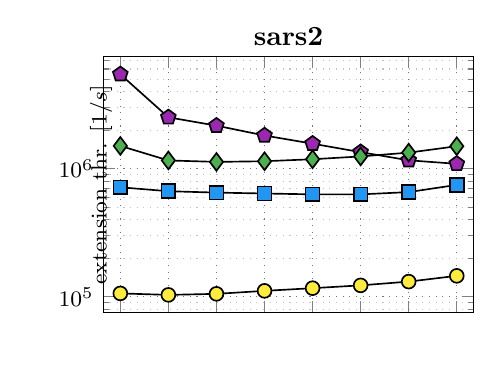
\begin{tikzpicture}[marks]
\begin{axis}[
    querystyle_raw_performance,
    xticklabels={},
    title={sars2},
    ylabel={extension thr. [$1/s$]},
    y label style={at={(0.05,0.5)}},
    xmode=log,
    ymode=log,
    xlabel={\vphantom{pattern length}}
]

%% MULTIPLOT(algo)
%% SELECT pattern_length AS x, ((num_patterns * pattern_length) / (time_count / 1000000000.0)) AS y, algo
%% FROM results_ext
%% WHERE text = 'sars2.ACGT.50Gi' AND dist_metr = 'exact' AND algo IN ('count_br_index', 'count_columba', 'count_columba_rlc', 'count_move_rb_move')
%% ORDER BY algo, pattern_length
\addplot[brindex] coordinates { (10,106347) (20,103544) (40,105505) (80,111336) (160,116834) (320,122866) (640,131476) (1280,145805) };
\addlegendentry{algo=count\_br\_index};
\addplot[columba] coordinates { (10,5.4612e+06) (20,2.51915e+06) (40,2.16882e+06) (80,1.8174e+06) (160,1.56849e+06) (320,1.34705e+06) (640,1.16334e+06) (1280,1.09218e+06) };
\addlegendentry{algo=count\_columba};
\addplot[bmove] coordinates { (10,716370) (20,667508) (40,651113) (80,640639) (160,630945) (320,630673) (640,657086) (1280,748013) };
\addlegendentry{algo=count\_columba\_rlc};
\addplot[moverb] coordinates { (10,1.50716e+06) (20,1.16072e+06) (40,1.13085e+06) (80,1.14412e+06) (160,1.186e+06) (320,1.24731e+06) (640,1.33569e+06) (1280,1.49866e+06) };
\addlegendentry{algo=count\_move\_rb\_move};

\legend{};
\end{axis}
\end{tikzpicture}
\end{subfigure}
\begin{subfigure}[b]{.31\textwidth}
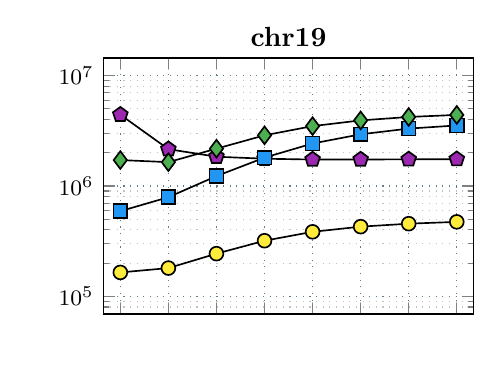
\begin{tikzpicture}[marks]
\begin{axis}[ymin=1e5,ymax=1e7,querystyle_raw_performance,
    xticklabels={},
    title={chr19},
    ylabel={\phantom{p}},
    xmode=log,
    ymode=log,
    xlabel={\vphantom{pattern length}}
]

%% MULTIPLOT(algo)
%% SELECT pattern_length AS x, ((num_patterns * pattern_length) / (time_count / 1000000000.0)) AS y, algo
%% FROM results_ext
%% WHERE text = 'chr19.ACGT.50Gi' AND dist_metr = 'exact' AND algo IN ('count_br_index', 'count_columba', 'count_columba_rlc', 'count_move_rb_move')
%% ORDER BY algo, pattern_length
\addplot[brindex] coordinates { (10,164515) (20,180177) (40,243478) (80,318880) (160,384117) (320,427749) (640,455063) (1280,472666) };
\addlegendentry{algo=count\_br\_index};
\addplot[columba] coordinates { (10,4.42761e+06) (20,2.15597e+06) (40,1.84222e+06) (80,1.76652e+06) (160,1.73629e+06) (320,1.73873e+06) (640,1.74286e+06) (1280,1.75064e+06) };
\addlegendentry{algo=count\_columba};
\addplot[bmove] coordinates { (10,591119) (20,791046) (40,1.22849e+06) (80,1.80732e+06) (160,2.42636e+06) (320,2.94103e+06) (640,3.31331e+06) (1280,3.53677e+06) };
\addlegendentry{algo=count\_columba\_rlc};
\addplot[moverb] coordinates { (10,1.71764e+06) (20,1.64447e+06) (40,2.17938e+06) (80,2.87845e+06) (160,3.48916e+06) (320,3.93049e+06) (640,4.22318e+06) (1280,4.40903e+06) };
\addlegendentry{algo=count\_move\_rb\_move};

\legend{};
\end{axis}
\end{tikzpicture}
\end{subfigure}
\begin{subfigure}[b]{.31\textwidth}
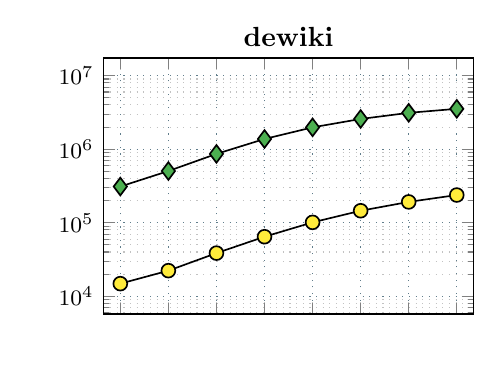
\begin{tikzpicture}[marks]
\begin{axis}[ymin=1e4,ymax=1e7,querystyle_raw_performance,
    xticklabels={},
    title={dewiki},
    ylabel={\phantom{p}},
    xmode=log,
    ymode=log,
    xlabel={\vphantom{pattern length}}
]

%% MULTIPLOT(algo)
%% SELECT pattern_length AS x, ((num_patterns * pattern_length) / (time_count / 1000000000.0)) AS y, algo
%% FROM results_ext
%% WHERE text = 'dewiki.50Gi' AND dist_metr = 'exact' AND algo IN ('count_br_index', 'count_columba', 'count_columba_rlc', 'count_move_rb_move')
%% ORDER BY algo, pattern_length
\addplot[brindex] coordinates { (10,14857.5) (20,22309.5) (40,38635.5) (80,64560.6) (160,101199) (320,145609) (640,191995) (1280,238160) };
\addlegendentry{algo=count\_br\_index};
\addplot[moverb] coordinates { (10,310647) (20,505017) (40,863676) (80,1.37774e+06) (160,1.98237e+06) (320,2.57758e+06) (640,3.12342e+06) (1280,3.54133e+06) };
\addlegendentry{algo=count\_move\_rb\_move};

\legend{};
\end{axis}
\end{tikzpicture}
\end{subfigure}

\vspace{-1.35cm}
\begin{subfigure}[b]{.31\textwidth}
\hspace*{-0.4cm}
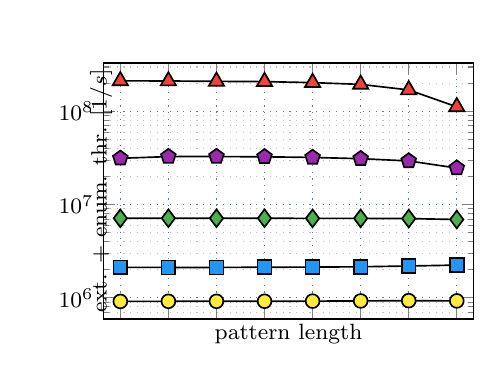
\begin{tikzpicture}[marks]
\begin{axis}[
    querystyle_raw_performance,
    xticklabels={},
    title={},
    ylabel={ext. + enum. thr. [$1/s$]},
    y label style={at={(0.05,0.5)}},
    xlabel={pattern length},
    xmode=log,
    ymode=log,
    title={\vphantom{Ig}}
]

%% MULTIPLOT(algo)
%% SELECT pattern_length AS x, ((num_patterns * pattern_length + (SELECT r.num_occurrences FROM results_ext r WHERE r.text = results_ext.text AND r.dist_metr = results_ext.dist_metr AND r.pattern_length = results_ext.pattern_length AND r.algo = 'locate_move_rb_move')) / (time_locate / 1000000000.0)) AS y, algo
%% FROM results_ext
%% WHERE text = 'sars2.ACGT.50Gi' AND dist_metr = 'exact' AND algo IN ('locate_br_index', 'locate_columba', 'locate_columba_rlc', 'locate_move_rb_move', 'locate_move_rb_rlzsa')
%% ORDER BY algo, pattern_length
\addplot[brindex] coordinates { (10,915315) (20,917937) (40,918297) (80,919292) (160,921903) (320,926433) (640,933304) (1280,927246) };
\addlegendentry{algo=locate\_br\_index};
\addplot[columba] coordinates { (10,3.14556e+07) (20,3.28118e+07) (40,3.28584e+07) (80,3.26389e+07) (160,3.21158e+07) (320,3.117e+07) (640,2.94662e+07) (1280,2.47202e+07) };
\addlegendentry{algo=locate\_columba};
\addplot[bmove] coordinates { (10,2.12638e+06) (20,2.1212e+06) (40,2.1206e+06) (80,2.13082e+06) (160,2.13777e+06) (320,2.15507e+06) (640,2.19682e+06) (1280,2.24603e+06) };
\addlegendentry{algo=locate\_columba\_rlc};
\addplot[moverb] coordinates { (10,7.14356e+06) (20,7.15541e+06) (40,7.14728e+06) (80,7.14705e+06) (160,7.12838e+06) (320,7.12797e+06) (640,7.08969e+06) (1280,6.93538e+06) };
\addlegendentry{algo=locate\_move\_rb\_move};
\addplot[moverbrlzsa] coordinates { (10,2.13429e+08) (20,2.12514e+08) (40,2.10573e+08) (80,2.09242e+08) (160,2.0407e+08) (320,1.95488e+08) (640,1.70454e+08) (1280,1.12239e+08) };
\addlegendentry{algo=locate\_move\_rb\_rlzsa};

\legend{};
\end{axis}
\end{tikzpicture}
\end{subfigure}
\begin{subfigure}[b]{.31\textwidth}
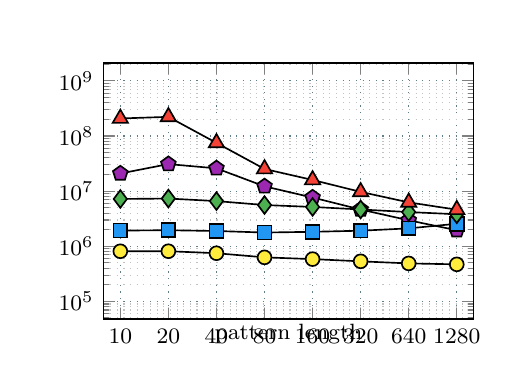
\begin{tikzpicture}[marks]
\begin{axis}[ymin=1e5,ymax=1e9,querystyle_raw_performance,
    title={},
    ylabel={\phantom{p}},
    xlabel={pattern length},
    xmode=log,
    ymode=log,
    title={\vphantom{Ig}}
]

%% MULTIPLOT(algo)
%% SELECT pattern_length AS x, ((num_patterns * pattern_length + (SELECT r.num_occurrences FROM results_ext r WHERE r.text = results_ext.text AND r.dist_metr = results_ext.dist_metr AND r.pattern_length = results_ext.pattern_length AND r.algo = 'locate_move_rb_move')) / (time_locate / 1000000000.0)) AS y, algo
%% FROM results_ext
%% WHERE text = 'chr19.ACGT.50Gi' AND dist_metr = 'exact' AND algo IN ('locate_br_index', 'locate_columba', 'locate_columba_rlc', 'locate_move_rb_move', 'locate_move_rb_rlzsa')
%% ORDER BY algo, pattern_length
\addplot[brindex] coordinates { (10,812380) (20,813890) (40,748472) (80,629913) (160,585132) (320,533508) (640,488867) (1280,470556) };
\addlegendentry{algo=locate\_br\_index};
\addplot[columba] coordinates { (10,2.08708e+07) (20,3.09203e+07) (40,2.58802e+07) (80,1.22141e+07) (160,7.65102e+06) (320,4.64134e+06) (640,2.95852e+06) (1280,1.95136e+06) };
\addlegendentry{algo=locate\_columba};
\addplot[bmove] coordinates { (10,1.92883e+06) (20,1.95496e+06) (40,1.89335e+06) (80,1.77426e+06) (160,1.83069e+06) (320,1.91574e+06) (640,2.11213e+06) (1280,2.56042e+06) };
\addlegendentry{algo=locate\_columba\_rlc};
\addplot[moverb] coordinates { (10,7.20505e+06) (20,7.33994e+06) (40,6.5964e+06) (80,5.59795e+06) (160,5.16698e+06) (320,4.64906e+06) (640,4.17185e+06) (1280,3.81075e+06) };
\addlegendentry{algo=locate\_move\_rb\_move};
\addplot[moverbrlzsa] coordinates { (10,2.07692e+08) (20,2.22262e+08) (40,7.49496e+07) (80,2.52268e+07) (160,1.59431e+07) (320,9.69483e+06) (640,6.25099e+06) (1280,4.60775e+06) };
\addlegendentry{algo=locate\_move\_rb\_rlzsa};

\legend{};
\end{axis}
\end{tikzpicture}
\end{subfigure}
\begin{subfigure}[b]{.31\textwidth}
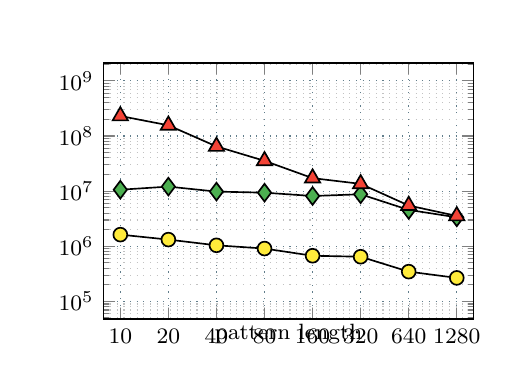
\begin{tikzpicture}[marks]
\begin{axis}[ymin=1e5,ymax=1e9,querystyle_raw_performance,
    title={},
    ylabel={\phantom{p}},
    xlabel={pattern length},
    xmode=log,
    ymode=log,
    title={\vphantom{Ig}}
]

%% MULTIPLOT(algo)
%% SELECT pattern_length AS x, ((num_patterns * pattern_length + (SELECT r.num_occurrences FROM results_ext r WHERE r.text = results_ext.text AND r.dist_metr = results_ext.dist_metr AND r.pattern_length = results_ext.pattern_length AND r.algo = 'locate_move_rb_move')) / (time_locate / 1000000000.0)) AS y, algo
%% FROM results_ext
%% WHERE text = 'dewiki.50Gi' AND dist_metr = 'exact' AND algo IN ('locate_br_index', 'locate_columba', 'locate_columba_rlc', 'locate_move_rb_move', 'locate_move_rb_rlzsa')
%% ORDER BY algo, pattern_length
\addplot[brindex] coordinates { (10,1.62629e+06) (20,1.32196e+06) (40,1.04129e+06) (80,909264) (160,673630) (320,646709) (640,347041) (1280,267153) };
\addlegendentry{algo=locate\_br\_index};
\addplot[moverb] coordinates { (10,1.06087e+07) (20,1.20776e+07) (40,9.80729e+06) (80,9.37695e+06) (160,8.16238e+06) (320,8.76773e+06) (640,4.56583e+06) (1280,3.34999e+06) };
\addlegendentry{algo=locate\_move\_rb\_move};
\addplot[moverbrlzsa] coordinates { (10,2.30363e+08) (20,1.56146e+08) (40,6.46538e+07) (80,3.544e+07) (160,1.7199e+07) (320,1.35478e+07) (640,5.48432e+06) (1280,3.55035e+06) };
\addlegendentry{algo=locate\_move\_rb\_rlzsa};

\legend{};
\end{axis}
\end{tikzpicture}
\end{subfigure}

\vspace*{-0.35cm}

\centering
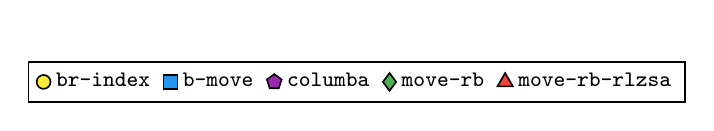
\begin{tikzpicture}[legendmarks]
\begin{axis}[legend,legend columns=5]
\addplot[brindex] coordinates { (0,0) };
\addlegendentry{\texttt{br-index}};
\addplot[bmove] coordinates { (0,0) };
\addlegendentry{\texttt{b-move}};
\addplot[columba] coordinates { (0,0) };
\addlegendentry{\texttt{columba}};
\addplot[moverb] coordinates { (0,0) };
\addlegendentry{\texttt{move-rb}};
\addplot[moverbrlzsa] coordinates { (0,0) };
\addlegendentry{\texttt{move-rb-rlzsa}};
\end{axis}
\end{tikzpicture}

\vspace*{-0.1cm}

\caption{\textup{[paper Figure D.1 --- \texttt{charts/raw\_performance.tex}, from
\texttt{results-ext.txt}]} Raw extension and $\SA$-interval enumeration throughput versus
pattern length.}
\label{fig:raw_performance}
\end{figure*}

\begin{figure*}[t]
\centering
% IMPORT-DATA results_apm results/results-apm.txt

\begin{subfigure}[h]{.31\textwidth}
\hspace*{-0.4cm}
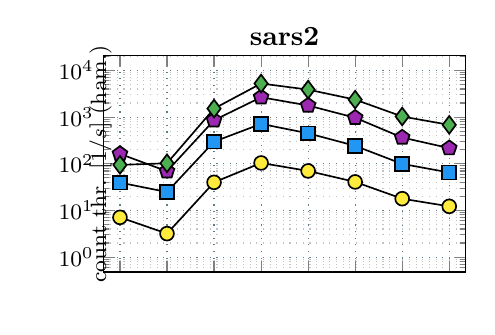
\begin{tikzpicture}[marks]
\begin{axis}[ymin=1e0,ymax=1e4,
    querystyle_apm_same_alg,
    xticklabels={},
    title={sars2},
    ylabel={count thr. [$1/s$] (ham.)},
    y label style={at={(0.05,0.5)}},
    xmode=log,
    ymode=log,
    xlabel={\vphantom{pattern length}}
]

%% MULTIPLOT(algo)
%% SELECT pattern_length AS x, exp(avg(ln((num_patterns * pattern_length) / (time_count / 1000000000.0)))) AS y, algo
%% FROM results_apm
%% WHERE text = 'sars2.ACGT.50Gi' AND dist_metr = 'hamming' AND algo IN ('count_br_index', 'count_columba_apm', 'count_columba_rlc_apm', 'count_move_rb_move') AND cigar = 0
%% GROUP BY algo, pattern_length
%% ORDER BY algo, pattern_length
\addplot[brindex] coordinates { (10,7.09937) (20,3.18105) (40,39.9209) (80,103.919) (160,70.0793) (320,40.7654) (640,17.807) (1280,12.2097) };
\addlegendentry{algo=count\_br\_index};
\addplot[columba] coordinates { (10,162.484) (20,68.958) (40,854.372) (80,2658.43) (160,1770.16) (320,967.053) (640,364.389) (1280,215.991) };
\addlegendentry{algo=count\_columba\_apm};
\addplot[bmove] coordinates { (10,39.3531) (20,24.7569) (40,297.055) (80,714.747) (160,449.145) (320,241.524) (640,99.1435) (1280,64.8617) };
\addlegendentry{algo=count\_columba\_rlc\_apm};
\addplot[moverb] coordinates { (10,94.4704) (20,102.286) (40,1516.64) (80,5233.77) (160,3875.03) (320,2364.14) (640,1028.44) (1280,680.715) };
\addlegendentry{algo=count\_move\_rb\_move};

\legend{};
\end{axis}
\end{tikzpicture}
\end{subfigure}
\begin{subfigure}[h]{.31\textwidth}
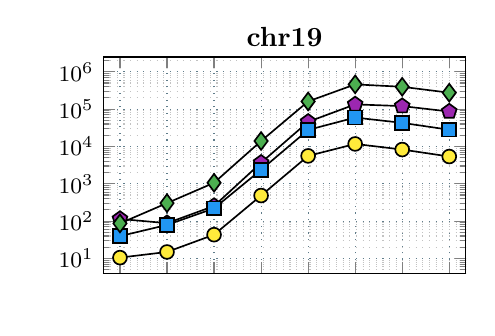
\begin{tikzpicture}[marks]
\begin{axis}[ymin=1e1,ymax=1e6,querystyle_apm_same_alg,
    xticklabels={},
    title={chr19},
    ylabel={\phantom{p}},
    xmode=log,
    ymode=log,
    xlabel={\vphantom{pattern length}}
]

%% MULTIPLOT(algo)
%% SELECT pattern_length AS x, exp(avg(ln((num_patterns * pattern_length) / (time_count / 1000000000.0)))) AS y, algo
%% FROM results_apm
%% WHERE text = 'chr19.ACGT.50Gi' AND dist_metr = 'hamming' AND algo IN ('count_br_index', 'count_columba_apm', 'count_columba_rlc_apm', 'count_move_rb_move') AND cigar = 0
%% GROUP BY algo, pattern_length
%% ORDER BY algo, pattern_length
\addplot[brindex] coordinates { (10,10.5277) (20,14.9093) (40,43.2777) (80,484.156) (160,5575.43) (320,11667.9) (640,8261.08) (1280,5370.1) };
\addlegendentry{algo=count\_br\_index};
\addplot[columba] coordinates { (10,114.224) (20,88.0285) (40,254.142) (80,3660.87) (160,45662.3) (320,133934) (640,120330) (1280,86119.4) };
\addlegendentry{algo=count\_columba\_apm};
\addplot[bmove] coordinates { (10,39.6006) (20,78.9444) (40,219.376) (80,2370.78) (160,27731.6) (320,59425.3) (640,42811.2) (1280,28025.2) };
\addlegendentry{algo=count\_columba\_rlc\_apm};
\addplot[moverb] coordinates { (10,86.7893) (20,303.283) (40,1062.78) (80,13976.2) (160,160543) (320,460172) (640,396108) (1280,275210) };
\addlegendentry{algo=count\_move\_rb\_move};

\legend{};
\end{axis}
\end{tikzpicture}
\end{subfigure}
\begin{subfigure}[h]{.31\textwidth}
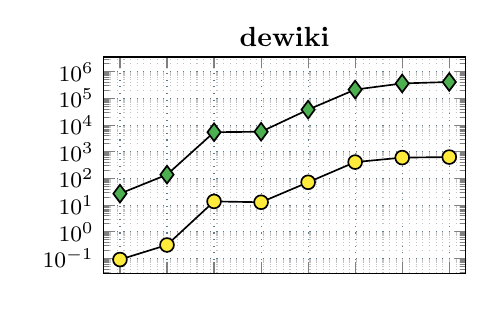
\begin{tikzpicture}[marks]
\begin{axis}[ymin=1e-1,ymax=1e6,querystyle_apm_same_alg,
    xticklabels={},
    title={dewiki},
    ylabel={\phantom{p}},
    xmode=log,
    ymode=log,
    xlabel={\vphantom{pattern length}}
]

%% MULTIPLOT(algo)
%% SELECT pattern_length AS x, exp(avg(ln((num_patterns * pattern_length) / (time_count / 1000000000.0)))) AS y, algo
%% FROM results_apm
%% WHERE text = 'dewiki.50Gi' AND dist_metr = 'hamming' AND algo IN ('count_br_index', 'count_columba_apm', 'count_columba_rlc_apm', 'count_move_rb_move') AND cigar = 0
%% GROUP BY algo, pattern_length
%% ORDER BY algo, pattern_length
\addplot[brindex] coordinates { (10,0.09096) (20,0.31995) (40,13.7572) (80,12.8202) (160,71.8213) (320,410.093) (640,605.101) (1280,633.656) };
\addlegendentry{algo=count\_br\_index};
\addplot[moverb] coordinates { (10,26.9207) (20,138.994) (40,5422.5) (80,5650.86) (160,37997.8) (320,215060) (640,365195) (1280,414752) };
\addlegendentry{algo=count\_move\_rb\_move};

\legend{};
\end{axis}
\end{tikzpicture}
\end{subfigure}

\vspace{-1.35cm}
\begin{subfigure}[h]{.31\textwidth}
\hspace*{-0.4cm}
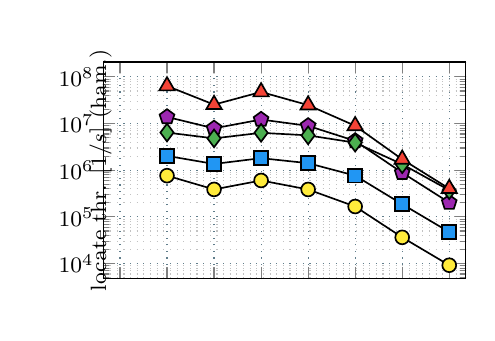
\begin{tikzpicture}[marks]
\begin{axis}[ymin=1e4,ymax=1e8,
    querystyle_apm_same_alg,
    xticklabels={},
    ylabel={locate thr. [$1/s$] (ham.)},
    y label style={at={(0.05,0.5)}},
    xmode=log,
    ymode=log,
    title={\vphantom{Ig}},
    xlabel={\vphantom{pattern length}}
]

%% MULTIPLOT(algo)
%% SELECT pattern_length AS x, exp(avg(ln((num_patterns * pattern_length + (SELECT r.num_occurrences FROM results_apm r WHERE r.text = results_apm.text AND r.dist_metr = results_apm.dist_metr AND r.max_mismatches = results_apm.max_mismatches AND r.pattern_length = results_apm.pattern_length AND r.cigar = 0 AND r.algo = 'locate_move_rb_move')) / (time_locate / 1000000000.0)))) AS y, algo
%% FROM results_apm
%% WHERE text = 'sars2.ACGT.50Gi' AND dist_metr = 'hamming' AND algo IN ('locate_br_index', 'locate_columba_apm', 'locate_columba_rlc_apm', 'locate_move_rb_move', 'locate_move_rb_rlzsa') AND cigar = 0
%% GROUP BY algo, pattern_length
%% ORDER BY algo, pattern_length
\addplot[brindex] coordinates { (20,766179) (40,388662) (80,604166) (160,387572) (320,167257) (640,36505.8) (1280,9224.58) };
\addlegendentry{algo=locate\_br\_index};
\addplot[columba] coordinates { (20,1.38963e+07) (40,7.90625e+06) (80,1.22127e+07) (160,8.94712e+06) (320,4.25719e+06) (640,887018) (1280,202842) };
\addlegendentry{algo=locate\_columba\_apm};
\addplot[bmove] coordinates { (20,2.03461e+06) (40,1.3655e+06) (80,1.81613e+06) (160,1.41855e+06) (320,767338) (640,187445) (1280,47460.3) };
\addlegendentry{algo=locate\_columba\_rlc\_apm};
\addplot[moverb] coordinates { (20,6.42541e+06) (40,4.8229e+06) (80,6.34363e+06) (160,5.59317e+06) (320,3.90036e+06) (640,1.34493e+06) (1280,374297) };
\addlegendentry{algo=locate\_move\_rb\_move};
\addplot[moverbrlzsa] coordinates { (20,6.39836e+07) (40,2.55151e+07) (80,4.76206e+07) (160,2.49084e+07) (320,8.97464e+06) (640,1.71732e+06) (1280,403913) };
\addlegendentry{algo=locate\_move\_rb\_rlzsa};

\legend{};
\end{axis}
\end{tikzpicture}
\end{subfigure}
\begin{subfigure}[h]{.31\textwidth}
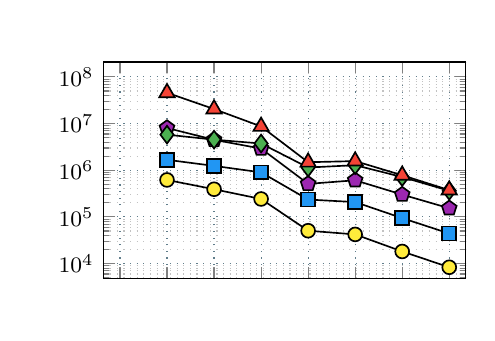
\begin{tikzpicture}[marks]
\begin{axis}[ymin=1e4,ymax=1e8,querystyle_apm_same_alg,
    xticklabels={},
    ylabel={\phantom{p}},
    xmode=log,
    ymode=log,
    title={\vphantom{Ig}},
    xlabel={\vphantom{pattern length}}
]

%% MULTIPLOT(algo)
%% SELECT pattern_length AS x, exp(avg(ln((num_patterns * pattern_length + (SELECT r.num_occurrences FROM results_apm r WHERE r.text = results_apm.text AND r.dist_metr = results_apm.dist_metr AND r.max_mismatches = results_apm.max_mismatches AND r.pattern_length = results_apm.pattern_length AND r.cigar = 0 AND r.algo = 'locate_move_rb_move')) / (time_locate / 1000000000.0)))) AS y, algo
%% FROM results_apm
%% WHERE text = 'chr19.ACGT.50Gi' AND dist_metr = 'hamming' AND algo IN ('locate_br_index', 'locate_columba_apm', 'locate_columba_rlc_apm', 'locate_move_rb_move', 'locate_move_rb_rlzsa') AND cigar = 0
%% GROUP BY algo, pattern_length
%% ORDER BY algo, pattern_length
\addplot[brindex] coordinates { (20,620052) (40,392082) (80,242366) (160,50652.4) (320,42208.6) (640,18192.4) (1280,8349.27) };
\addlegendentry{algo=locate\_br\_index};
\addplot[columba] coordinates { (20,8.05411e+06) (40,4.49173e+06) (80,2.91382e+06) (160,511188) (320,609543) (640,301092) (1280,153385) };
\addlegendentry{algo=locate\_columba\_apm};
\addplot[bmove] coordinates { (20,1.67671e+06) (40,1.2409e+06) (80,901697) (160,235695) (320,208184) (640,94256.1) (1280,44173.3) };
\addlegendentry{algo=locate\_columba\_rlc\_apm};
\addplot[moverb] coordinates { (20,5.79088e+06) (40,4.52647e+06) (80,3.74344e+06) (160,1.14393e+06) (320,1.28509e+06) (640,716054) (1280,363177) };
\addlegendentry{algo=locate\_move\_rb\_move};
\addplot[moverbrlzsa] coordinates { (20,4.58147e+07) (40,2.04906e+07) (80,8.69383e+06) (160,1.48744e+06) (320,1.57242e+06) (640,782034) (1280,375528) };
\addlegendentry{algo=locate\_move\_rb\_rlzsa};

\legend{};
\end{axis}
\end{tikzpicture}
\end{subfigure}
\begin{subfigure}[h]{.31\textwidth}
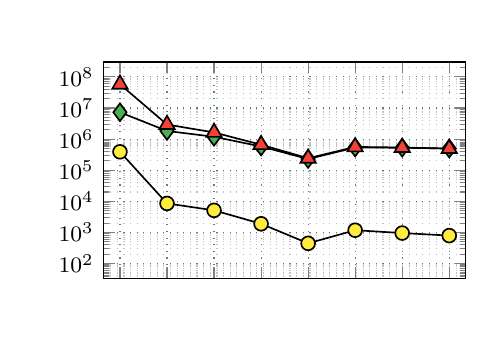
\begin{tikzpicture}[marks]
\begin{axis}[ymin=1e2,ymax=1e8,querystyle_apm_same_alg,
    xticklabels={},
    ylabel={\phantom{p}},
    xmode=log,
    ymode=log,
    title={\vphantom{Ig}},
    xlabel={\vphantom{pattern length}}
]

%% MULTIPLOT(algo)
%% SELECT pattern_length AS x, exp(avg(ln((num_patterns * pattern_length + (SELECT r.num_occurrences FROM results_apm r WHERE r.text = results_apm.text AND r.dist_metr = results_apm.dist_metr AND r.max_mismatches = results_apm.max_mismatches AND r.pattern_length = results_apm.pattern_length AND r.cigar = 0 AND r.algo = 'locate_move_rb_move')) / (time_locate / 1000000000.0)))) AS y, algo
%% FROM results_apm
%% WHERE text = 'dewiki.50Gi' AND dist_metr = 'hamming' AND algo IN ('locate_br_index', 'locate_columba_apm', 'locate_columba_rlc_apm', 'locate_move_rb_move', 'locate_move_rb_rlzsa') AND cigar = 0
%% GROUP BY algo, pattern_length
%% ORDER BY algo, pattern_length
\addplot[brindex] coordinates { (10,391514) (20,8592.88) (40,5149.25) (80,1904.56) (160,447.753) (320,1183.81) (640,958.862) (1280,795.16) };
\addlegendentry{algo=locate\_br\_index};
\addplot[moverb] coordinates { (10,7.31258e+06) (20,1.8323e+06) (40,1.19248e+06) (80,581436) (160,230011) (320,538879) (640,529707) (1280,499884) };
\addlegendentry{algo=locate\_move\_rb\_move};
\addplot[moverbrlzsa] coordinates { (10,5.81153e+07) (20,2.95186e+06) (40,1.64334e+06) (80,663769) (160,242821) (320,562836) (640,538545) (1280,495446) };
\addlegendentry{algo=locate\_move\_rb\_rlzsa};

\legend{};
\end{axis}
\end{tikzpicture}
\end{subfigure}

\vspace{-1.35cm}
\begin{subfigure}[h]{.31\textwidth}
\hspace*{-0.4cm}
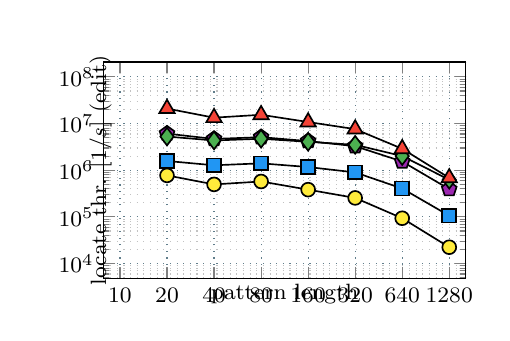
\begin{tikzpicture}[marks]
\begin{axis}[ymin=1e4,ymax=1e8,
    querystyle_apm_same_alg,
    xlabel={pattern length},
    ylabel={locate thr. [$1/s$] (edit)},
    y label style={at={(0.05,0.5)}},
    xmode=log,
    ymode=log,,
    title={\vphantom{Ig}}
]

%% MULTIPLOT(algo)
%% SELECT pattern_length AS x, exp(avg(ln((num_patterns * pattern_length + (SELECT r.num_occurrences FROM results_apm r WHERE r.text = results_apm.text AND r.dist_metr = results_apm.dist_metr AND r.max_mismatches = results_apm.max_mismatches AND r.pattern_length = results_apm.pattern_length AND r.cigar = 0 AND r.algo = 'locate_move_rb_move')) / (time_locate / 1000000000.0)))) AS y, algo
%% FROM results_apm
%% WHERE text = 'sars2.ACGT.50Gi' AND dist_metr = 'edit' AND algo IN ('locate_br_index', 'locate_columba_apm', 'locate_columba_rlc_apm', 'locate_move_rb_move', 'locate_move_rb_rlzsa') AND cigar = 0
%% GROUP BY algo, pattern_length
%% ORDER BY algo, pattern_length
\addplot[brindex] coordinates { (20,776626) (40,497316) (80,574773) (160,384076) (320,255540) (640,93778.4) (1280,22438.6) };
\addlegendentry{algo=locate\_br\_index};
\addplot[columba] coordinates { (20,6.09854e+06) (40,4.68503e+06) (80,5.11717e+06) (160,4.2166e+06) (320,3.28113e+06) (640,1.53974e+06) (1280,394180) };
\addlegendentry{algo=locate\_columba\_apm};
\addplot[bmove] coordinates { (20,1.5811e+06) (40,1.27802e+06) (80,1.4073e+06) (160,1.17252e+06) (320,899462) (640,406199) (1280,106200) };
\addlegendentry{algo=locate\_columba\_rlc\_apm};
\addplot[moverb] coordinates { (20,5.27563e+06) (40,4.34548e+06) (80,4.732e+06) (160,4.06949e+06) (320,3.50736e+06) (640,2.01783e+06) (1280,625990) };
\addlegendentry{algo=locate\_move\_rb\_move};
\addplot[moverbrlzsa] coordinates { (20,2.09949e+07) (40,1.33959e+07) (80,1.54486e+07) (160,1.0804e+07) (320,7.61368e+06) (640,2.88973e+06) (1280,686311) };
\addlegendentry{algo=locate\_move\_rb\_rlzsa};

\legend{};
\end{axis}
\end{tikzpicture}
\end{subfigure}
\begin{subfigure}[h]{.31\textwidth}
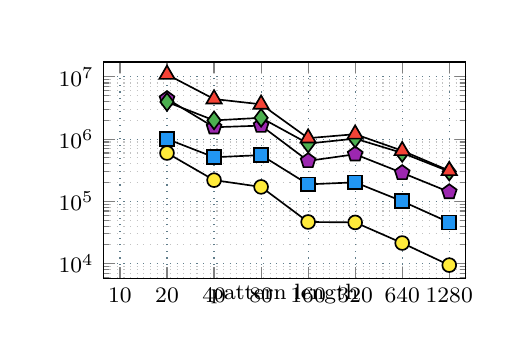
\begin{tikzpicture}[marks]
\begin{axis}[ymin=1e4,ymax=1e7,querystyle_apm_same_alg,
    xlabel={pattern length},
    ylabel={\phantom{p}},
    xmode=log,
    ymode=log,,
    title={\vphantom{Ig}}
]

%% MULTIPLOT(algo)
%% SELECT pattern_length AS x, exp(avg(ln((num_patterns * pattern_length + (SELECT r.num_occurrences FROM results_apm r WHERE r.text = results_apm.text AND r.dist_metr = results_apm.dist_metr AND r.max_mismatches = results_apm.max_mismatches AND r.pattern_length = results_apm.pattern_length AND r.cigar = 0 AND r.algo = 'locate_move_rb_move')) / (time_locate / 1000000000.0)))) AS y, algo
%% FROM results_apm
%% WHERE text = 'chr19.ACGT.50Gi' AND dist_metr = 'edit' AND algo IN ('locate_br_index', 'locate_columba_apm', 'locate_columba_rlc_apm', 'locate_move_rb_move', 'locate_move_rb_rlzsa') AND cigar = 0
%% GROUP BY algo, pattern_length
%% ORDER BY algo, pattern_length
\addplot[brindex] coordinates { (20,598620) (40,219363) (80,170844) (160,46640.8) (320,45913.4) (640,21415.3) (1280,9454.12) };
\addlegendentry{algo=locate\_br\_index};
\addplot[columba] coordinates { (20,4.44785e+06) (40,1.55333e+06) (80,1.64936e+06) (160,447369) (320,571527) (640,287285) (1280,141573) };
\addlegendentry{algo=locate\_columba\_apm};
\addplot[bmove] coordinates { (20,1.00742e+06) (40,512059) (80,553981) (160,187781) (320,202163) (640,100528) (1280,45864.7) };
\addlegendentry{algo=locate\_columba\_rlc\_apm};
\addplot[moverb] coordinates { (20,3.96068e+06) (40,2.00234e+06) (80,2.20246e+06) (160,849777) (320,1.01968e+06) (640,600377) (1280,301809) };
\addlegendentry{algo=locate\_move\_rb\_move};
\addplot[moverbrlzsa] coordinates { (20,1.09534e+07) (40,4.41251e+06) (80,3.62966e+06) (160,1.03771e+06) (320,1.20102e+06) (640,652162) (1280,311544) };
\addlegendentry{algo=locate\_move\_rb\_rlzsa};

\legend{};
\end{axis}
\end{tikzpicture}
\end{subfigure}
\begin{subfigure}[h]{.31\textwidth}
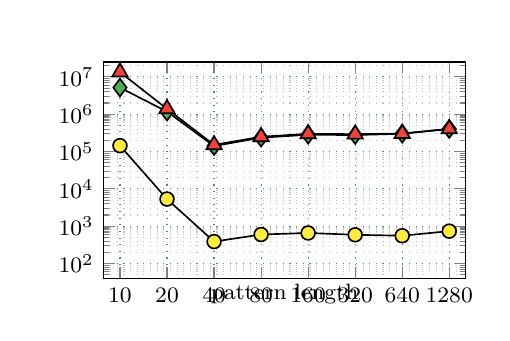
\begin{tikzpicture}[marks]
\begin{axis}[ymin=1e2,ymax=1e7,querystyle_apm_same_alg,
    xlabel={pattern length},
    ylabel={\phantom{p}},
    xmode=log,
    ymode=log,,
    title={\vphantom{Ig}}
]

%% MULTIPLOT(algo)
%% SELECT pattern_length AS x, exp(avg(ln((num_patterns * pattern_length + (SELECT r.num_occurrences FROM results_apm r WHERE r.text = results_apm.text AND r.dist_metr = results_apm.dist_metr AND r.max_mismatches = results_apm.max_mismatches AND r.pattern_length = results_apm.pattern_length AND r.cigar = 0 AND r.algo = 'locate_move_rb_move')) / (time_locate / 1000000000.0)))) AS y, algo
%% FROM results_apm
%% WHERE text = 'dewiki.50Gi' AND dist_metr = 'edit' AND algo IN ('locate_br_index', 'locate_columba_apm', 'locate_columba_rlc_apm', 'locate_move_rb_move', 'locate_move_rb_rlzsa') AND cigar = 0
%% GROUP BY algo, pattern_length
%% ORDER BY algo, pattern_length
\addplot[brindex] coordinates { (10,144366) (20,5348.39) (40,388.956) (80,601.027) (160,661.227) (320,590.96) (640,557.738) (1280,740.151) };
\addlegendentry{algo=locate\_br\_index};
\addplot[moverb] coordinates { (10,5.16966e+06) (20,1.17815e+06) (40,140602) (80,235716) (160,282849) (320,277565) (640,300730) (1280,403425) };
\addlegendentry{algo=locate\_move\_rb\_move};
\addplot[moverbrlzsa] coordinates { (10,1.34878e+07) (20,1.39526e+06) (40,151395) (80,249623) (160,299757) (320,293016) (640,305030) (1280,406089) };
\addlegendentry{algo=locate\_move\_rb\_rlzsa};

\legend{};
\end{axis}
\end{tikzpicture}
\end{subfigure}

\vspace*{-0.35cm}

\centering
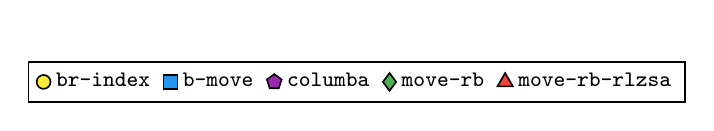
\begin{tikzpicture}[legendmarks]
\begin{axis}[legend,legend columns=5]
\addplot[brindex] coordinates { (0,0) };
\addlegendentry{\texttt{br-index}};
\addplot[bmove] coordinates { (0,0) };
\addlegendentry{\texttt{b-move}};
\addplot[columba] coordinates { (0,0) };
\addlegendentry{\texttt{columba}};
\addplot[moverb] coordinates { (0,0) };
\addlegendentry{\texttt{move-rb}};
\addplot[moverbrlzsa] coordinates { (0,0) };
\addlegendentry{\texttt{move-rb-rlzsa}};
\end{axis}
\end{tikzpicture}

\vspace*{-0.1cm}

\caption{\textup{[paper Figure E.1 --- \texttt{charts/apm-same-alg.tex}, from
\texttt{results-apm.txt}]} APM query throughput as a geometric mean over the results for
$k \in \{4, 7, 10, 13\}$. All indexes use our optimized APM algorithms.}
\label{fig:apm_same_alg}
\end{figure*}

% paper Figures F.1-F.4: native APM algorithms, one figure per k
\begin{figure*}[p]
\centering
% IMPORT-DATA results_apm results/results-apm.txt
% SQL CREATE TEMP VIEW apm AS SELECT a.text, a.dist_metr, a.algo, a.max_mismatches, a.pattern_length, (a.num_patterns * a.pattern_length) / (a.time_count / 1000.0) AS count_thr, (a.num_patterns * a.pattern_length + (SELECT r.num_occurrences FROM results_apm r WHERE r.text = a.text AND r.dist_metr = a.dist_metr AND r.max_mismatches = a.max_mismatches AND r.pattern_length = a.pattern_length AND r.cigar = 0 AND r.algo = 'locate_move_rb_move')) / (a.time_locate / 1000.0) AS locate_thr FROM results_apm a WHERE a.cigar = 0

\begin{subfigure}[b]{.31\textwidth}
\hspace*{-0.7cm}
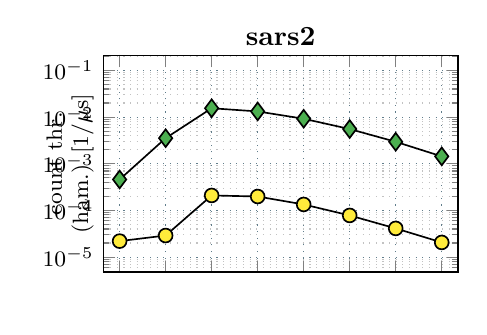
\begin{tikzpicture}[marks]
\begin{axis}[ymin=1e-5,ymax=1e-1,
    querystyle_kfig,
    title={sars2},
    ylabel={count thr.\\ (ham.) [1/$\mu$s]},
    y label style={at={(0.0,0.5)},align=center},
    xmin=10,
    xmax=1280,
    xticklabels={},
    xmode=log,
    ymode=log,
    xlabel={\vphantom{pattern length}}
]

%% MULTIPLOT(algo)
%% SELECT pattern_length AS x, exp(avg(ln(count_thr))) AS y, algo
%% FROM apm
%% WHERE text = 'sars2.ACGT.50Gi' AND dist_metr = 'hamming' AND algo IN ('count_br_index_native', 'count_move_rb_move') AND max_mismatches = 4
%% GROUP BY algo, pattern_length
%% ORDER BY algo, pattern_length
\addplot[brindex] coordinates { (10,2.19709e-05) (20,2.89395e-05) (40,0.00020914) (80,0.000198459) (160,0.000134097) (320,7.80153e-05) (640,4.11102e-05) (1280,2.05946e-05) };
\addlegendentry{algo=count\_br\_index\_native};
\addplot[moverb] coordinates { (10,0.000459527) (20,0.00352825) (40,0.0154566) (80,0.0131948) (160,0.00920761) (320,0.00553387) (640,0.00295338) (1280,0.00143675) };
\addlegendentry{algo=count\_move\_rb\_move};

\legend{};
\end{axis}
\end{tikzpicture}
\end{subfigure}
\begin{subfigure}[b]{.31\textwidth}
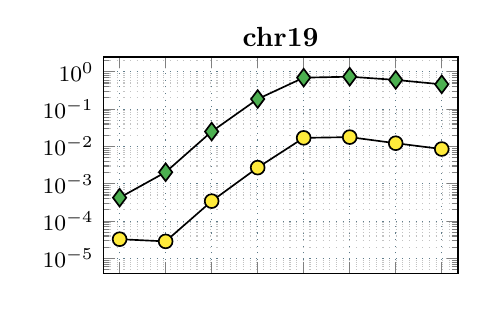
\begin{tikzpicture}[marks]
\begin{axis}[ymin=1e-5,ymax=1e0,querystyle_kfig,
    title={chr19},
    ylabel={\phantom{p}},
    xmin=10,
    xmax=1280,
    xticklabels={},
    xmode=log,
    ymode=log,
    xlabel={\vphantom{pattern length}}
]

%% MULTIPLOT(algo)
%% SELECT pattern_length AS x, exp(avg(ln(count_thr))) AS y, algo
%% FROM apm
%% WHERE text = 'chr19.ACGT.50Gi' AND dist_metr = 'hamming' AND algo IN ('count_br_index_native', 'count_move_rb_move') AND max_mismatches = 4
%% GROUP BY algo, pattern_length
%% ORDER BY algo, pattern_length
\addplot[brindex] coordinates { (10,3.28163e-05) (20,2.86382e-05) (40,0.00034288) (80,0.00270969) (160,0.0169777) (320,0.0177846) (640,0.0121985) (1280,0.00852923) };
\addlegendentry{algo=count\_br\_index\_native};
\addplot[moverb] coordinates { (10,0.000424701) (20,0.00204283) (40,0.0250445) (80,0.186175) (160,0.696222) (320,0.73817) (640,0.605838) (1280,0.460457) };
\addlegendentry{algo=count\_move\_rb\_move};

\legend{};
\end{axis}
\end{tikzpicture}
\end{subfigure}
\begin{subfigure}[b]{.31\textwidth}
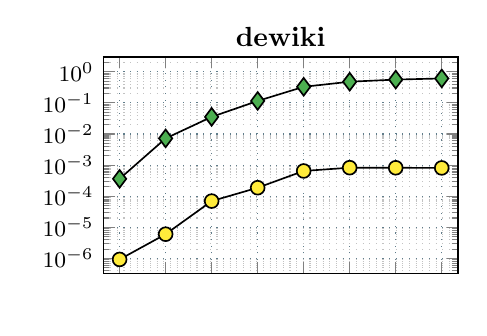
\begin{tikzpicture}[marks]
\begin{axis}[ymin=1e-6,ymax=1e0,querystyle_kfig,
    title={dewiki},
    ylabel={\phantom{p}},
    xmin=10,
    xmax=1280,
    xticklabels={},
    xmode=log,
    ymode=log,
    xlabel={\vphantom{pattern length}}
]

%% MULTIPLOT(algo)
%% SELECT pattern_length AS x, exp(avg(ln(count_thr))) AS y, algo
%% FROM apm
%% WHERE text = 'dewiki.50Gi' AND dist_metr = 'hamming' AND algo IN ('count_br_index_native', 'count_move_rb_move') AND max_mismatches = 4
%% GROUP BY algo, pattern_length
%% ORDER BY algo, pattern_length
\addplot[brindex] coordinates { (10,9.30524e-07) (20,6.03164e-06) (40,6.97353e-05) (80,0.000187695) (160,0.000648553) (320,0.000826678) (640,0.000820943) (1280,0.000812535) };
\addlegendentry{algo=count\_br\_index\_native};
\addplot[moverb] coordinates { (10,0.000362932) (20,0.00722399) (40,0.0355053) (80,0.115473) (160,0.328826) (320,0.479355) (640,0.560841) (1280,0.611009) };
\addlegendentry{algo=count\_move\_rb\_move};

\legend{};
\end{axis}
\end{tikzpicture}
\end{subfigure}

\vspace{-1.35cm}
\begin{subfigure}[b]{.31\textwidth}
\hspace*{-0.7cm}
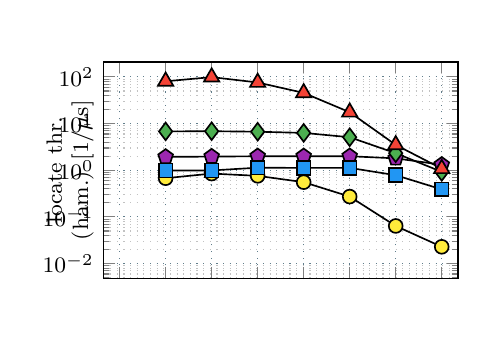
\begin{tikzpicture}[marks]
\begin{axis}[ymin=1e-2,ymax=1e2,
    querystyle_kfig,
    ylabel={locate thr.\\ (ham.) [1/$\mu$s]},
    y label style={at={(0.0,0.5)},align=center},
    xmin=10,
    xmax=1280,
    xticklabels={},
    xmode=log,
    ymode=log,
    title={\vphantom{Ig}},
    xlabel={\vphantom{pattern length}}
]

%% MULTIPLOT(algo)
%% SELECT pattern_length AS x, exp(avg(ln(locate_thr))) AS y, algo
%% FROM apm
%% WHERE text = 'sars2.ACGT.50Gi' AND dist_metr = 'hamming' AND algo IN ('locate_br_index_native', 'locate_columba', 'locate_columba_rlc', 'locate_move_rb_move', 'locate_move_rb_rlzsa') AND max_mismatches = 4
%% GROUP BY algo, pattern_length
%% ORDER BY algo, pattern_length
\addplot[brindex] coordinates { (20,0.675933) (40,0.849427) (80,0.759015) (160,0.556007) (320,0.272855) (640,0.0640838) (1280,0.0228983) };
\addlegendentry{algo=locate\_br\_index\_native};
\addplot[columba] coordinates { (20,1.9373) (40,1.9639) (80,1.99574) (160,1.99421) (320,1.9984) (640,1.80008) (1280,1.31244) };
\addlegendentry{algo=locate\_columba};
\addplot[bmove] coordinates { (20,0.988408) (40,0.991161) (80,1.1352) (160,1.12303) (320,1.1238) (640,0.784414) (1280,0.389176) };
\addlegendentry{algo=locate\_columba\_rlc};
\addplot[moverb] coordinates { (20,6.80191) (40,6.86713) (80,6.70023) (160,6.32287) (320,5.10282) (640,2.32239) (1280,0.924499) };
\addlegendentry{algo=locate\_move\_rb\_move};
\addplot[moverbrlzsa] coordinates { (20,80.6563) (40,99.0588) (80,76.0882) (160,45.5184) (320,17.5174) (640,3.50105) (1280,1.08221) };
\addlegendentry{algo=locate\_move\_rb\_rlzsa};

\legend{};
\end{axis}
\end{tikzpicture}
\end{subfigure}
\begin{subfigure}[b]{.31\textwidth}
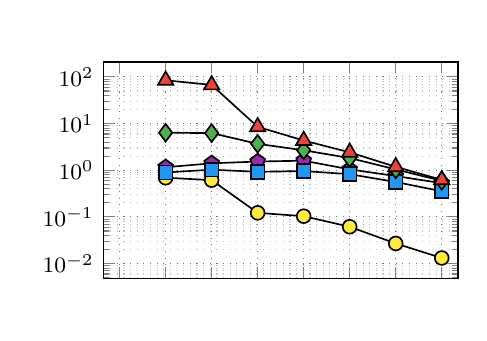
\begin{tikzpicture}[marks]
\begin{axis}[ymin=1e-2,ymax=1e2,querystyle_kfig,
    ylabel={\phantom{p}},
    xmin=10,
    xmax=1280,
    xticklabels={},
    xmode=log,
    ymode=log,
    title={\vphantom{Ig}},
    xlabel={\vphantom{pattern length}}
]

%% MULTIPLOT(algo)
%% SELECT pattern_length AS x, exp(avg(ln(locate_thr))) AS y, algo
%% FROM apm
%% WHERE text = 'chr19.ACGT.50Gi' AND dist_metr = 'hamming' AND algo IN ('locate_br_index_native', 'locate_columba', 'locate_columba_rlc', 'locate_move_rb_move', 'locate_move_rb_rlzsa') AND max_mismatches = 4
%% GROUP BY algo, pattern_length
%% ORDER BY algo, pattern_length
\addplot[brindex] coordinates { (20,0.69268) (40,0.614168) (80,0.122316) (160,0.103758) (320,0.0615708) (640,0.0270059) (1280,0.0131952) };
\addlegendentry{algo=locate\_br\_index\_native};
\addplot[columba] coordinates { (20,1.1605) (40,1.40851) (80,1.53934) (160,1.6042) (320,1.0457) (640,0.751617) (1280,0.529152) };
\addlegendentry{algo=locate\_columba};
\addplot[bmove] coordinates { (20,0.898605) (40,1.02896) (80,0.926489) (160,0.962157) (320,0.824057) (640,0.560872) (1280,0.355151) };
\addlegendentry{algo=locate\_columba\_rlc};
\addplot[moverb] coordinates { (20,6.37893) (40,6.26065) (80,3.68791) (160,2.6794) (320,1.83046) (640,1.04502) (1280,0.594867) };
\addlegendentry{algo=locate\_move\_rb\_move};
\addplot[moverbrlzsa] coordinates { (20,84.7002) (40,67.4534) (80,8.5387) (160,4.3445) (320,2.42243) (640,1.1874) (1280,0.624085) };
\addlegendentry{algo=locate\_move\_rb\_rlzsa};

\legend{};
\end{axis}
\end{tikzpicture}
\end{subfigure}
\begin{subfigure}[b]{.31\textwidth}
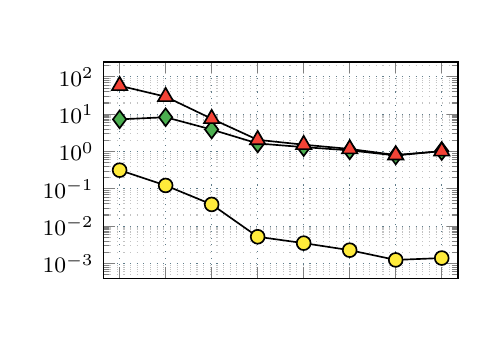
\begin{tikzpicture}[marks]
\begin{axis}[ymin=1e-3,ymax=1e2,querystyle_kfig,
    ylabel={\phantom{p}},
    xmin=10,
    xmax=1280,
    xticklabels={},
    xmode=log,
    ymode=log,
    title={\vphantom{Ig}},
    xlabel={\vphantom{pattern length}}
]

%% MULTIPLOT(algo)
%% SELECT pattern_length AS x, exp(avg(ln(locate_thr))) AS y, algo
%% FROM apm
%% WHERE text = 'dewiki.50Gi' AND dist_metr = 'hamming' AND algo IN ('locate_br_index_native', 'locate_columba', 'locate_columba_rlc', 'locate_move_rb_move', 'locate_move_rb_rlzsa') AND max_mismatches = 4
%% GROUP BY algo, pattern_length
%% ORDER BY algo, pattern_length
\addplot[brindex] coordinates { (10,0.318378) (20,0.123975) (40,0.038455) (80,0.0052307) (160,0.0035344) (320,0.00228963) (640,0.0012547) (1280,0.00140827) };
\addlegendentry{algo=locate\_br\_index\_native};
\addplot[moverb] coordinates { (10,7.31258) (20,8.32097) (40,3.89776) (80,1.6513) (160,1.31769) (320,1.07876) (640,0.789537) (1280,1.0322) };
\addlegendentry{algo=locate\_move\_rb\_move};
\addplot[moverbrlzsa] coordinates { (10,58.1153) (20,29.59) (40,7.59809) (80,2.06854) (160,1.53158) (320,1.17793) (640,0.810177) (1280,1.02473) };
\addlegendentry{algo=locate\_move\_rb\_rlzsa};

\legend{};
\end{axis}
\end{tikzpicture}
\end{subfigure}

\vspace{-1.35cm}
\begin{subfigure}[b]{.31\textwidth}
\hspace*{-0.7cm}
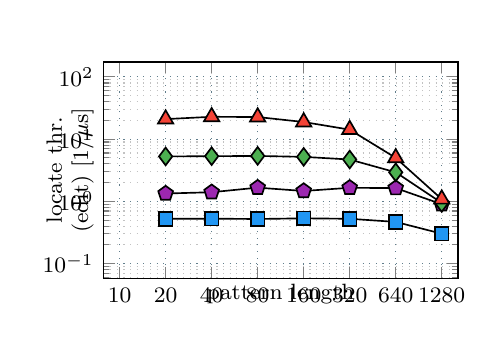
\begin{tikzpicture}[marks]
\begin{axis}[ymin=1e-1,ymax=1e2,
    querystyle_kfig,
    ylabel={locate thr.\\ (edit) [1/$\mu$s]},
    y label style={at={(0.0,0.5)},align=center},
    xmin=10,
    xmax=1280,
    xlabel={pattern length},
    xmode=log,
    ymode=log,
    title={\vphantom{Ig}}
]

%% MULTIPLOT(algo)
%% SELECT pattern_length AS x, exp(avg(ln(locate_thr))) AS y, algo
%% FROM apm
%% WHERE text = 'sars2.ACGT.50Gi' AND dist_metr = 'edit' AND algo IN ('locate_columba', 'locate_columba_rlc', 'locate_move_rb_move', 'locate_move_rb_rlzsa') AND max_mismatches = 4
%% GROUP BY algo, pattern_length
%% ORDER BY algo, pattern_length
\addplot[columba] coordinates { (20,1.33696) (40,1.40358) (80,1.66197) (160,1.46907) (320,1.65369) (640,1.63496) (1280,0.900762) };
\addlegendentry{algo=locate\_columba};
\addplot[bmove] coordinates { (20,0.523839) (40,0.527205) (80,0.521015) (160,0.533955) (320,0.525206) (640,0.467673) (1280,0.302525) };
\addlegendentry{algo=locate\_columba\_rlc};
\addplot[moverb] coordinates { (20,5.27563) (40,5.32147) (80,5.3756) (160,5.19526) (320,4.70726) (640,2.932) (1280,0.943634) };
\addlegendentry{algo=locate\_move\_rb\_move};
\addplot[moverbrlzsa] coordinates { (20,20.9949) (40,22.8852) (80,22.6716) (160,18.865) (320,14.2163) (640,5.00375) (1280,1.08542) };
\addlegendentry{algo=locate\_move\_rb\_rlzsa};

\legend{};
\end{axis}
\end{tikzpicture}
\end{subfigure}
\begin{subfigure}[b]{.31\textwidth}
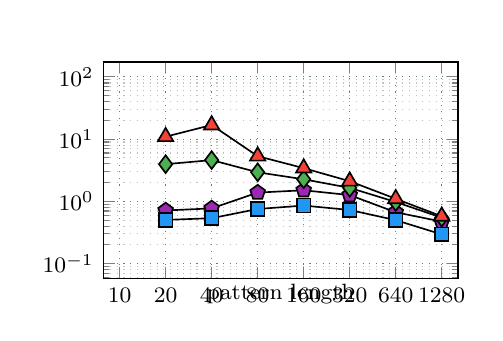
\begin{tikzpicture}[marks]
\begin{axis}[ymin=1e-1,ymax=1e2,querystyle_kfig,
    ylabel={\phantom{p}},
    xmin=10,
    xmax=1280,
    xlabel={pattern length},
    xmode=log,
    ymode=log,
    title={\vphantom{Ig}}
]

%% MULTIPLOT(algo)
%% SELECT pattern_length AS x, exp(avg(ln(locate_thr))) AS y, algo
%% FROM apm
%% WHERE text = 'chr19.ACGT.50Gi' AND dist_metr = 'edit' AND algo IN ('locate_columba', 'locate_columba_rlc', 'locate_move_rb_move', 'locate_move_rb_rlzsa') AND max_mismatches = 4
%% GROUP BY algo, pattern_length
%% ORDER BY algo, pattern_length
\addplot[columba] coordinates { (20,0.714669) (40,0.7716) (80,1.38412) (160,1.50846) (320,1.26261) (640,0.668534) (1280,0.473091) };
\addlegendentry{algo=locate\_columba};
\addplot[bmove] coordinates { (20,0.503202) (40,0.537056) (80,0.754164) (160,0.856875) (320,0.727268) (640,0.499424) (1280,0.294791) };
\addlegendentry{algo=locate\_columba\_rlc};
\addplot[moverb] coordinates { (20,3.96068) (40,4.60671) (80,2.93385) (160,2.26569) (320,1.64984) (640,0.978064) (1280,0.547116) };
\addlegendentry{algo=locate\_move\_rb\_move};
\addplot[moverbrlzsa] coordinates { (20,10.9534) (40,16.8865) (80,5.33006) (160,3.42276) (320,2.11036) (640,1.1013) (1280,0.575407) };
\addlegendentry{algo=locate\_move\_rb\_rlzsa};

\legend{};
\end{axis}
\end{tikzpicture}
\end{subfigure}
\begin{subfigure}[b]{.31\textwidth}
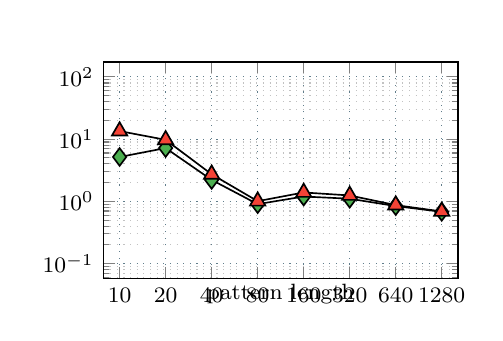
\begin{tikzpicture}[marks]
\begin{axis}[ymin=1e-1,ymax=1e2,querystyle_kfig,
    ylabel={\phantom{p}},
    xmin=10,
    xmax=1280,
    xlabel={pattern length},
    xmode=log,
    ymode=log,
    title={\vphantom{Ig}}
]

%% MULTIPLOT(algo)
%% SELECT pattern_length AS x, exp(avg(ln(locate_thr))) AS y, algo
%% FROM apm
%% WHERE text = 'dewiki.50Gi' AND dist_metr = 'edit' AND algo IN ('locate_columba', 'locate_columba_rlc', 'locate_move_rb_move', 'locate_move_rb_rlzsa') AND max_mismatches = 4
%% GROUP BY algo, pattern_length
%% ORDER BY algo, pattern_length
\addplot[moverb] coordinates { (10,5.16966) (20,7.1933) (40,2.21285) (80,0.902516) (160,1.19696) (320,1.10304) (640,0.8404) (1280,0.678855) };
\addlegendentry{algo=locate\_move\_rb\_move};
\addplot[moverbrlzsa] coordinates { (10,13.4878) (20,9.75258) (40,2.72512) (80,1.00716) (160,1.39104) (320,1.24501) (640,0.871189) (1280,0.68895) };
\addlegendentry{algo=locate\_move\_rb\_rlzsa};

\legend{};
\end{axis}
\end{tikzpicture}
\end{subfigure}


\vspace*{-0.35cm}

\centering
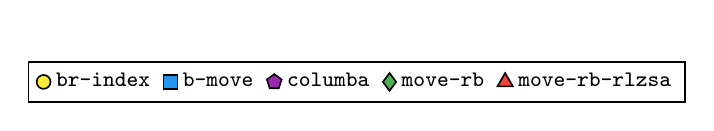
\begin{tikzpicture}[legendmarks]
\begin{axis}[legend,legend columns=5]
\addplot[brindex] coordinates { (0,0) };
\addlegendentry{\texttt{br-index}};
\addplot[bmove] coordinates { (0,0) };
\addlegendentry{\texttt{b-move}};
\addplot[columba] coordinates { (0,0) };
\addlegendentry{\texttt{columba}};
\addplot[moverb] coordinates { (0,0) };
\addlegendentry{\texttt{move-rb}};
\addplot[moverbrlzsa] coordinates { (0,0) };
\addlegendentry{\texttt{move-rb-rlzsa}};
\end{axis}
\end{tikzpicture}

\vspace*{-0.1cm}

\caption{\textup{[paper Figure F.1 --- \texttt{charts/apm\_native\_k4.tex}]} APM query
throughput for $k = 4$. All indexes use their native APM algorithms.}
\label{fig:apm_native_k4}

% IMPORT-DATA results_apm results/results-apm.txt
% SQL CREATE TEMP VIEW apm AS SELECT a.text, a.dist_metr, a.algo, a.max_mismatches, a.pattern_length, (a.num_patterns * a.pattern_length) / (a.time_count / 1000.0) AS count_thr, (a.num_patterns * a.pattern_length + (SELECT r.num_occurrences FROM results_apm r WHERE r.text = a.text AND r.dist_metr = a.dist_metr AND r.max_mismatches = a.max_mismatches AND r.pattern_length = a.pattern_length AND r.cigar = 0 AND r.algo = 'locate_move_rb_move')) / (a.time_locate / 1000.0) AS locate_thr FROM results_apm a WHERE a.cigar = 0

\begin{subfigure}[b]{.31\textwidth}
\hspace*{-0.7cm}
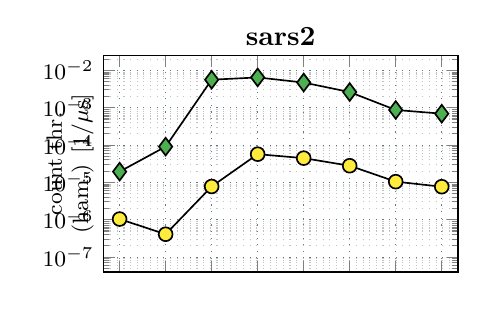
\begin{tikzpicture}[marks]
\begin{axis}[ymin=1e-7,ymax=1e-2,
    querystyle_kfig,
    title={sars2},
    ylabel={count thr.\\ (ham.) [1/$\mu$s]},
    y label style={at={(0.0,0.5)},align=center},
    xmin=10,
    xmax=1280,
    xticklabels={},
    xmode=log,
    ymode=log,
    xlabel={\vphantom{pattern length}}
]

%% MULTIPLOT(algo)
%% SELECT pattern_length AS x, exp(avg(ln(count_thr))) AS y, algo
%% FROM apm
%% WHERE text = 'sars2.ACGT.50Gi' AND dist_metr = 'hamming' AND algo IN ('count_br_index_native', 'count_move_rb_move') AND max_mismatches = 7
%% GROUP BY algo, pattern_length
%% ORDER BY algo, pattern_length
\addplot[brindex] coordinates { (10,1.04223e-06) (20,4.09062e-07) (40,7.77287e-06) (80,5.70538e-05) (160,4.46482e-05) (320,2.79597e-05) (640,1.04701e-05) (1280,7.66606e-06) };
\addlegendentry{algo=count\_br\_index\_native};
\addplot[moverb] coordinates { (10,1.94214e-05) (20,9.07842e-05) (40,0.00562784) (80,0.00648198) (160,0.00472656) (320,0.00263037) (640,0.000871668) (1280,0.000692836) };
\addlegendentry{algo=count\_move\_rb\_move};

\legend{};
\end{axis}
\end{tikzpicture}
\end{subfigure}
\begin{subfigure}[b]{.31\textwidth}
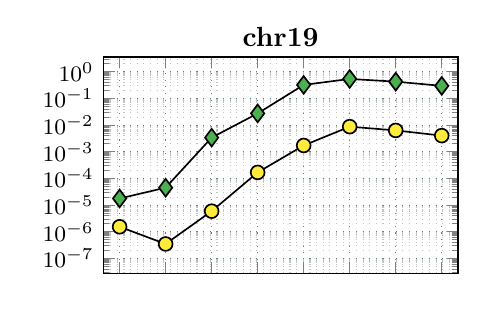
\begin{tikzpicture}[marks]
\begin{axis}[ymin=1e-7,ymax=1e0,querystyle_kfig,
    title={chr19},
    ylabel={\phantom{p}},
    xmin=10,
    xmax=1280,
    xticklabels={},
    xmode=log,
    ymode=log,
    xlabel={\vphantom{pattern length}}
]

%% MULTIPLOT(algo)
%% SELECT pattern_length AS x, exp(avg(ln(count_thr))) AS y, algo
%% FROM apm
%% WHERE text = 'chr19.ACGT.50Gi' AND dist_metr = 'hamming' AND algo IN ('count_br_index_native', 'count_move_rb_move') AND max_mismatches = 7
%% GROUP BY algo, pattern_length
%% ORDER BY algo, pattern_length
\addplot[brindex] coordinates { (10,1.54035e-06) (20,3.49585e-07) (40,5.93273e-06) (80,0.00016867) (160,0.00172435) (320,0.00874931) (640,0.00632812) (1280,0.00403415) };
\addlegendentry{algo=count\_br\_index\_native};
\addplot[moverb] coordinates { (10,1.77357e-05) (20,4.50262e-05) (40,0.00339664) (80,0.0274337) (160,0.322002) (320,0.53869) (640,0.426646) (1280,0.296565) };
\addlegendentry{algo=count\_move\_rb\_move};

\legend{};
\end{axis}
\end{tikzpicture}
\end{subfigure}
\begin{subfigure}[b]{.31\textwidth}
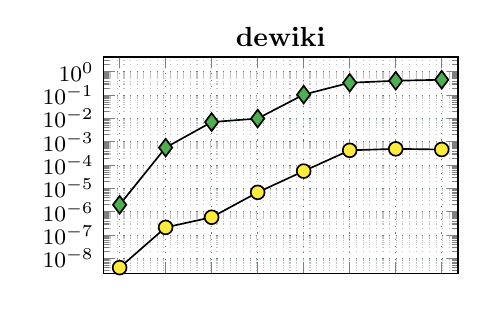
\begin{tikzpicture}[marks]
\begin{axis}[ymin=1e-8,ymax=1e0,querystyle_kfig,
    title={dewiki},
    ylabel={\phantom{p}},
    xmin=10,
    xmax=1280,
    xticklabels={},
    xmode=log,
    ymode=log,
    xlabel={\vphantom{pattern length}}
]

%% MULTIPLOT(algo)
%% SELECT pattern_length AS x, exp(avg(ln(count_thr))) AS y, algo
%% FROM apm
%% WHERE text = 'dewiki.50Gi' AND dist_metr = 'hamming' AND algo IN ('count_br_index_native', 'count_move_rb_move') AND max_mismatches = 7
%% GROUP BY algo, pattern_length
%% ORDER BY algo, pattern_length
\addplot[brindex] coordinates { (10,4.04742e-09) (20,2.13699e-07) (40,5.83513e-07) (80,6.79829e-06) (160,5.53013e-05) (320,0.000430937) (640,0.000497252) (1280,0.000466629) };
\addlegendentry{algo=count\_br\_index\_native};
\addplot[moverb] coordinates { (10,1.99686e-06) (20,0.000563964) (40,0.006993) (80,0.0099148) (160,0.105362) (320,0.337911) (640,0.412754) (1280,0.456294) };
\addlegendentry{algo=count\_move\_rb\_move};

\legend{};
\end{axis}
\end{tikzpicture}
\end{subfigure}

\vspace{-1.35cm}
\begin{subfigure}[b]{.31\textwidth}
\hspace*{-0.7cm}
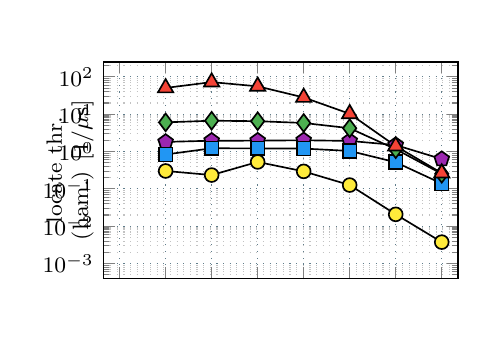
\begin{tikzpicture}[marks]
\begin{axis}[ymin=1e-3,ymax=1e2,
    querystyle_kfig,
    ylabel={locate thr.\\ (ham.) [1/$\mu$s]},
    y label style={at={(0.0,0.5)},align=center},
    xmin=10,
    xmax=1280,
    xticklabels={},
    xmode=log,
    ymode=log,
    title={\vphantom{Ig}},
    xlabel={\vphantom{pattern length}}
]

%% MULTIPLOT(algo)
%% SELECT pattern_length AS x, exp(avg(ln(locate_thr))) AS y, algo
%% FROM apm
%% WHERE text = 'sars2.ACGT.50Gi' AND dist_metr = 'hamming' AND algo IN ('locate_br_index_native', 'locate_columba', 'locate_columba_rlc', 'locate_move_rb_move', 'locate_move_rb_rlzsa') AND max_mismatches = 7
%% GROUP BY algo, pattern_length
%% ORDER BY algo, pattern_length
\addplot[brindex] coordinates { (20,0.302776) (40,0.235299) (80,0.528356) (160,0.295258) (320,0.126916) (640,0.0208552) (1280,0.00376055) };
\addlegendentry{algo=locate\_br\_index\_native};
\addplot[columba] coordinates { (20,1.81635) (40,1.95772) (80,1.96443) (160,2.01085) (320,1.93255) (640,1.49767) (1280,0.631024) };
\addlegendentry{algo=locate\_columba};
\addplot[bmove] coordinates { (20,0.836707) (40,1.22659) (80,1.21813) (160,1.2044) (320,1.04134) (640,0.518687) (1280,0.139173) };
\addlegendentry{algo=locate\_columba\_rlc};
\addplot[moverb] coordinates { (20,6.06974) (40,6.71857) (80,6.52241) (160,5.84843) (320,4.23066) (640,1.15997) (1280,0.254308) };
\addlegendentry{algo=locate\_move\_rb\_move};
\addplot[moverbrlzsa] coordinates { (20,50.7574) (40,72.6055) (80,56.0231) (160,28.2323) (320,10.3053) (640,1.40594) (1280,0.265735) };
\addlegendentry{algo=locate\_move\_rb\_rlzsa};

\legend{};
\end{axis}
\end{tikzpicture}
\end{subfigure}
\begin{subfigure}[b]{.31\textwidth}
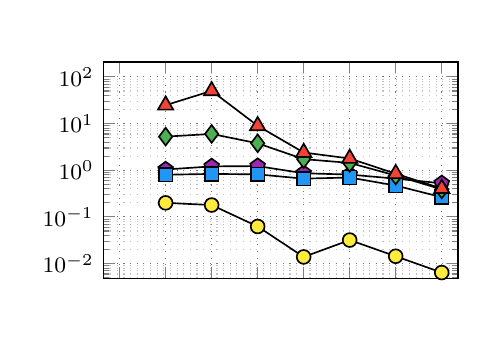
\begin{tikzpicture}[marks]
\begin{axis}[ymin=1e-2,ymax=1e2,querystyle_kfig,
    ylabel={\phantom{p}},
    xmin=10,
    xmax=1280,
    xticklabels={},
    xmode=log,
    ymode=log,
    title={\vphantom{Ig}},
    xlabel={\vphantom{pattern length}}
]

%% MULTIPLOT(algo)
%% SELECT pattern_length AS x, exp(avg(ln(locate_thr))) AS y, algo
%% FROM apm
%% WHERE text = 'chr19.ACGT.50Gi' AND dist_metr = 'hamming' AND algo IN ('locate_br_index_native', 'locate_columba', 'locate_columba_rlc', 'locate_move_rb_move', 'locate_move_rb_rlzsa') AND max_mismatches = 7
%% GROUP BY algo, pattern_length
%% ORDER BY algo, pattern_length
\addplot[brindex] coordinates { (20,0.200439) (40,0.179801) (80,0.062434) (160,0.0139013) (320,0.0319544) (640,0.0143688) (1280,0.00642364) };
\addlegendentry{algo=locate\_br\_index\_native};
\addplot[columba] coordinates { (20,1.03952) (40,1.20989) (80,1.2279) (160,0.862847) (320,0.808049) (640,0.661456) (1280,0.524872) };
\addlegendentry{algo=locate\_columba};
\addplot[bmove] coordinates { (20,0.801917) (40,0.834989) (80,0.817109) (160,0.661366) (320,0.699043) (640,0.470339) (1280,0.264848) };
\addlegendentry{algo=locate\_columba\_rlc};
\addplot[moverb] coordinates { (20,5.25705) (40,6.0081) (80,3.7806) (160,1.7323) (320,1.43843) (640,0.771241) (1280,0.389456) };
\addlegendentry{algo=locate\_move\_rb\_move};
\addplot[moverbrlzsa] coordinates { (20,24.7814) (40,50.3216) (80,8.98017) (160,2.39821) (320,1.78808) (640,0.845708) (1280,0.405428) };
\addlegendentry{algo=locate\_move\_rb\_rlzsa};

\legend{};
\end{axis}
\end{tikzpicture}
\end{subfigure}
\begin{subfigure}[b]{.31\textwidth}
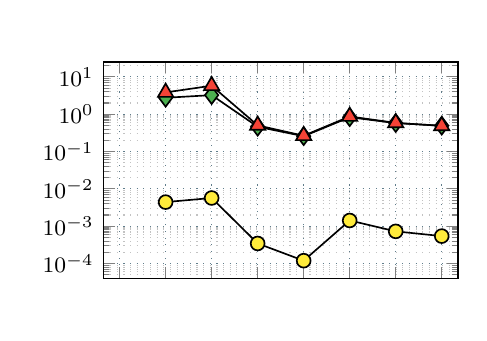
\begin{tikzpicture}[marks]
\begin{axis}[ymin=1e-4,ymax=1e1,querystyle_kfig,
    ylabel={\phantom{p}},
    xmin=10,
    xmax=1280,
    xticklabels={},
    xmode=log,
    ymode=log,
    title={\vphantom{Ig}},
    xlabel={\vphantom{pattern length}}
]

%% MULTIPLOT(algo)
%% SELECT pattern_length AS x, exp(avg(ln(locate_thr))) AS y, algo
%% FROM apm
%% WHERE text = 'dewiki.50Gi' AND dist_metr = 'hamming' AND algo IN ('locate_br_index_native', 'locate_columba', 'locate_columba_rlc', 'locate_move_rb_move', 'locate_move_rb_rlzsa') AND max_mismatches = 7
%% GROUP BY algo, pattern_length
%% ORDER BY algo, pattern_length
\addplot[brindex] coordinates { (20,0.00444148) (40,0.00571822) (80,0.000346262) (160,0.000119767) (320,0.0014295) (640,0.000729952) (1280,0.00054556) };
\addlegendentry{algo=locate\_br\_index\_native};
\addplot[moverb] coordinates { (20,2.76106) (40,3.25883) (80,0.462798) (160,0.258071) (320,0.832719) (640,0.579994) (1280,0.493812) };
\addlegendentry{algo=locate\_move\_rb\_move};
\addplot[moverbrlzsa] coordinates { (20,3.84945) (40,5.81706) (80,0.503909) (160,0.266206) (320,0.872488) (640,0.588171) (1280,0.48813) };
\addlegendentry{algo=locate\_move\_rb\_rlzsa};

\legend{};
\end{axis}
\end{tikzpicture}
\end{subfigure}

\vspace{-1.35cm}
\begin{subfigure}[b]{.31\textwidth}
\hspace*{-0.7cm}
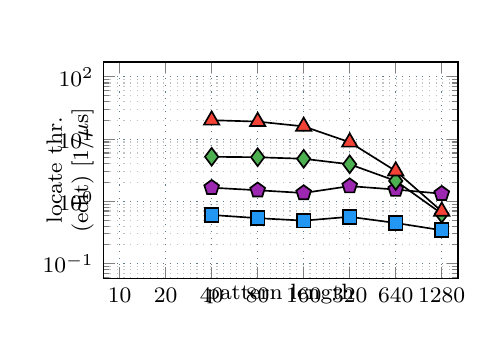
\begin{tikzpicture}[marks]
\begin{axis}[ymin=1e-1,ymax=1e2,
    querystyle_kfig,
    ylabel={locate thr.\\ (edit) [1/$\mu$s]},
    y label style={at={(0.0,0.5)},align=center},
    xmin=10,
    xmax=1280,
    xlabel={pattern length},
    xmode=log,
    ymode=log,
    title={\vphantom{Ig}}
]

%% MULTIPLOT(algo)
%% SELECT pattern_length AS x, exp(avg(ln(locate_thr))) AS y, algo
%% FROM apm
%% WHERE text = 'sars2.ACGT.50Gi' AND dist_metr = 'edit' AND algo IN ('locate_columba', 'locate_columba_rlc', 'locate_move_rb_move', 'locate_move_rb_rlzsa') AND max_mismatches = 7
%% GROUP BY algo, pattern_length
%% ORDER BY algo, pattern_length
\addplot[columba] coordinates { (40,1.65947) (80,1.50991) (160,1.36394) (320,1.75924) (640,1.5482) (1280,1.32866) };
\addlegendentry{algo=locate\_columba};
\addplot[bmove] coordinates { (40,0.604917) (80,0.537818) (160,0.490426) (320,0.564832) (640,0.449794) (1280,0.343778) };
\addlegendentry{algo=locate\_columba\_rlc};
\addplot[moverb] coordinates { (40,5.21088) (80,5.1212) (160,4.83643) (320,3.94729) (640,2.13388) (1280,0.634582) };
\addlegendentry{algo=locate\_move\_rb\_move};
\addplot[moverbrlzsa] coordinates { (40,20.1697) (80,19.14) (160,16.045) (320,8.92404) (640,3.07553) (1280,0.691719) };
\addlegendentry{algo=locate\_move\_rb\_rlzsa};

\legend{};
\end{axis}
\end{tikzpicture}
\end{subfigure}
\begin{subfigure}[b]{.31\textwidth}
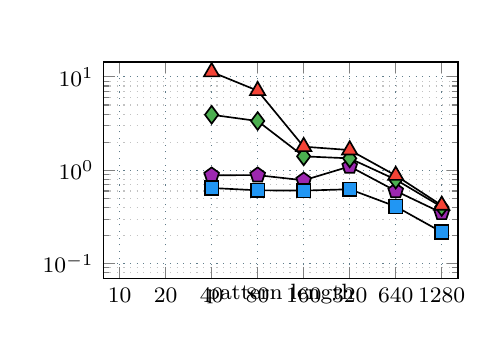
\begin{tikzpicture}[marks]
\begin{axis}[ymin=1e-1,ymax=1e1,querystyle_kfig,
    ylabel={\phantom{p}},
    xmin=10,
    xmax=1280,
    xlabel={pattern length},
    xmode=log,
    ymode=log,
    title={\vphantom{Ig}}
]

%% MULTIPLOT(algo)
%% SELECT pattern_length AS x, exp(avg(ln(locate_thr))) AS y, algo
%% FROM apm
%% WHERE text = 'chr19.ACGT.50Gi' AND dist_metr = 'edit' AND algo IN ('locate_columba', 'locate_columba_rlc', 'locate_move_rb_move', 'locate_move_rb_rlzsa') AND max_mismatches = 7
%% GROUP BY algo, pattern_length
%% ORDER BY algo, pattern_length
\addplot[columba] coordinates { (40,0.885679) (80,0.886445) (160,0.780817) (320,1.09911) (640,0.600897) (1280,0.349545) };
\addlegendentry{algo=locate\_columba};
\addplot[bmove] coordinates { (40,0.645896) (80,0.609665) (160,0.605401) (320,0.626056) (640,0.409261) (1280,0.217572) };
\addlegendentry{algo=locate\_columba\_rlc};
\addplot[moverb] coordinates { (40,3.93365) (80,3.3696) (160,1.40968) (320,1.34144) (640,0.79442) (1280,0.404656) };
\addlegendentry{algo=locate\_move\_rb\_move};
\addplot[moverbrlzsa] coordinates { (40,11.3094) (80,7.11781) (160,1.79001) (320,1.64661) (640,0.879297) (1280,0.420379) };
\addlegendentry{algo=locate\_move\_rb\_rlzsa};

\legend{};
\end{axis}
\end{tikzpicture}
\end{subfigure}
\begin{subfigure}[b]{.31\textwidth}
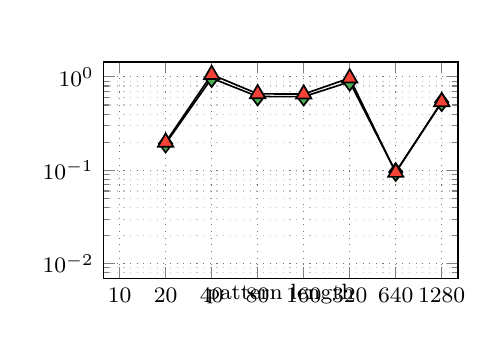
\begin{tikzpicture}[marks]
\begin{axis}[ymin=1e-2,ymax=1e0,querystyle_kfig,
    ylabel={\phantom{p}},
    xmin=10,
    xmax=1280,
    xlabel={pattern length},
    xmode=log,
    ymode=log,
    title={\vphantom{Ig}}
]

%% MULTIPLOT(algo)
%% SELECT pattern_length AS x, exp(avg(ln(locate_thr))) AS y, algo
%% FROM apm
%% WHERE text = 'dewiki.50Gi' AND dist_metr = 'edit' AND algo IN ('locate_columba', 'locate_columba_rlc', 'locate_move_rb_move', 'locate_move_rb_rlzsa') AND max_mismatches = 7
%% GROUP BY algo, pattern_length
%% ORDER BY algo, pattern_length
\addplot[moverb] coordinates { (20,0.192962) (40,0.969372) (80,0.616502) (160,0.614152) (320,0.886057) (640,0.0956561) (1280,0.535502) };
\addlegendentry{algo=locate\_move\_rb\_move};
\addplot[moverbrlzsa] coordinates { (20,0.199614) (40,1.06017) (80,0.659404) (160,0.654607) (320,0.971912) (640,0.0948591) (1280,0.542032) };
\addlegendentry{algo=locate\_move\_rb\_rlzsa};

\legend{};
\end{axis}
\end{tikzpicture}
\end{subfigure}


\vspace*{-0.35cm}

\centering
\begin{tikzpicture}[legendmarks]
\begin{axis}[legend,legend columns=5]
\addplot[brindex] coordinates { (0,0) };
\addlegendentry{\texttt{br-index}};
\addplot[bmove] coordinates { (0,0) };
\addlegendentry{\texttt{b-move}};
\addplot[columba] coordinates { (0,0) };
\addlegendentry{\texttt{columba}};
\addplot[moverb] coordinates { (0,0) };
\addlegendentry{\texttt{move-rb}};
\addplot[moverbrlzsa] coordinates { (0,0) };
\addlegendentry{\texttt{move-rb-rlzsa}};
\end{axis}
\end{tikzpicture}

\vspace*{-0.1cm}

\caption{\textup{[paper Figure F.2 --- \texttt{charts/apm\_native\_k7.tex}]} APM query
throughput for $k = 7$. All indexes use their native APM algorithms.}
\label{fig:apm_native_k7}
\end{figure*}

\begin{figure*}[p]
\centering
% IMPORT-DATA results_apm results/results-apm.txt
% SQL CREATE TEMP VIEW apm AS SELECT a.text, a.dist_metr, a.algo, a.max_mismatches, a.pattern_length, (a.num_patterns * a.pattern_length) / (a.time_count / 1000.0) AS count_thr, (a.num_patterns * a.pattern_length + (SELECT r.num_occurrences FROM results_apm r WHERE r.text = a.text AND r.dist_metr = a.dist_metr AND r.max_mismatches = a.max_mismatches AND r.pattern_length = a.pattern_length AND r.cigar = 0 AND r.algo = 'locate_move_rb_move')) / (a.time_locate / 1000.0) AS locate_thr FROM results_apm a WHERE a.cigar = 0

\begin{subfigure}[b]{.31\textwidth}
\hspace*{-0.7cm}
\begin{tikzpicture}[marks]
\begin{axis}[ymin=1e-8,ymax=1e-2,
    querystyle_kfig,
    title={sars2},
    ylabel={count thr.\\ (ham.) [1/$\mu$s]},
    y label style={at={(0.0,0.5)},align=center},
    xmin=20,
    xmax=1280,
    xticklabels={},
    xmode=log,
    ymode=log,
    xlabel={\vphantom{pattern length}}
]

%% MULTIPLOT(algo)
%% SELECT pattern_length AS x, exp(avg(ln(count_thr))) AS y, algo
%% FROM apm
%% WHERE text = 'sars2.ACGT.50Gi' AND dist_metr = 'hamming' AND algo IN ('count_br_index_native', 'count_move_rb_move') AND max_mismatches = 10
%% GROUP BY algo, pattern_length
%% ORDER BY algo, pattern_length
\addplot[brindex] coordinates { (20,3.9282e-08) (40,4.36174e-07) (80,1.72959e-05) (160,2.14994e-05) (320,1.36997e-05) (640,6.30627e-06) (1280,4.06648e-06) };
\addlegendentry{algo=count\_br\_index\_native};
\addplot[moverb] coordinates { (20,3.34099e-06) (40,0.000580258) (80,0.00355255) (160,0.00288859) (320,0.00159914) (640,0.000625298) (1280,0.000388159) };
\addlegendentry{algo=count\_move\_rb\_move};

\legend{};
\end{axis}
\end{tikzpicture}
\end{subfigure}
\begin{subfigure}[b]{.31\textwidth}
\begin{tikzpicture}[marks]
\begin{axis}[ymin=1e-7,ymax=1e0,querystyle_kfig,
    title={chr19},
    ylabel={\phantom{p}},
    xmin=40,
    xmax=1280,
    xticklabels={},
    xmode=log,
    ymode=log,
    xlabel={\vphantom{pattern length}}
]

%% MULTIPLOT(algo)
%% SELECT pattern_length AS x, exp(avg(ln(count_thr))) AS y, algo
%% FROM apm
%% WHERE text = 'chr19.ACGT.50Gi' AND dist_metr = 'hamming' AND algo IN ('count_br_index_native', 'count_move_rb_move') AND max_mismatches = 10
%% GROUP BY algo, pattern_length
%% ORDER BY algo, pattern_length
\addplot[brindex] coordinates { (40,3.22904e-07) (80,1.87922e-05) (160,0.000297538) (320,0.00348318) (640,0.00423287) (1280,0.00263624) };
\addlegendentry{algo=count\_br\_index\_native};
\addplot[moverb] coordinates { (40,0.000279537) (80,0.00441657) (160,0.0901944) (320,0.395952) (640,0.338796) (1280,0.226748) };
\addlegendentry{algo=count\_move\_rb\_move};

\legend{};
\end{axis}
\end{tikzpicture}
\end{subfigure}
\begin{subfigure}[b]{.31\textwidth}
\begin{tikzpicture}[marks]
\begin{axis}[ymin=1e-8,ymax=1e0,querystyle_kfig,
    title={dewiki},
    ylabel={\phantom{p}},
    xmin=20,
    xmax=1280,
    xticklabels={},
    xmode=log,
    ymode=log,
    xlabel={\vphantom{pattern length}}
]

%% MULTIPLOT(algo)
%% SELECT pattern_length AS x, exp(avg(ln(count_thr))) AS y, algo
%% FROM apm
%% WHERE text = 'dewiki.50Gi' AND dist_metr = 'hamming' AND algo IN ('count_br_index_native', 'count_move_rb_move') AND max_mismatches = 10
%% GROUP BY algo, pattern_length
%% ORDER BY algo, pattern_length
\addplot[brindex] coordinates { (20,1.12694e-08) (40,2.21203e-07) (80,6.58151e-07) (160,4.89634e-06) (320,0.000148799) (640,0.000311909) (1280,0.000320432) };
\addlegendentry{algo=count\_br\_index\_native};
\addplot[moverb] coordinates { (20,1.49871e-05) (40,0.00339733) (80,0.00166026) (160,0.0165442) (320,0.179842) (640,0.318118) (1280,0.353568) };
\addlegendentry{algo=count\_move\_rb\_move};

\legend{};
\end{axis}
\end{tikzpicture}
\end{subfigure}

\vspace{-1.35cm}
\begin{subfigure}[b]{.31\textwidth}
\hspace*{-0.7cm}
\begin{tikzpicture}[marks]
\begin{axis}[ymin=1e-3,ymax=1e2,
    querystyle_kfig,
    ylabel={locate thr.\\ (ham.) [1/$\mu$s]},
    y label style={at={(0.0,0.5)},align=center},
    xmin=20,
    xmax=1280,
    xticklabels={},
    xmode=log,
    ymode=log,
    title={\vphantom{Ig}},
    xlabel={\vphantom{pattern length}}
]

%% MULTIPLOT(algo)
%% SELECT pattern_length AS x, exp(avg(ln(locate_thr))) AS y, algo
%% FROM apm
%% WHERE text = 'sars2.ACGT.50Gi' AND dist_metr = 'hamming' AND algo IN ('locate_br_index_native', 'locate_columba', 'locate_columba_rlc', 'locate_move_rb_move', 'locate_move_rb_rlzsa') AND max_mismatches = 10
%% GROUP BY algo, pattern_length
%% ORDER BY algo, pattern_length
\addplot[brindex] coordinates { (40,0.0176609) (80,0.255442) (160,0.164193) (320,0.0651244) (640,0.0199513) (1280,0.0036871) };
\addlegendentry{algo=locate\_br\_index\_native};
\addplot[columba] coordinates { (40,1.86594) (80,1.97593) (160,1.93237) (320,1.7609) (640,1.32846) (1280,0.535421) };
\addlegendentry{algo=locate\_columba};
\addplot[bmove] coordinates { (40,1.05253) (80,1.07137) (160,0.96696) (320,0.72016) (640,0.374772) (1280,0.105138) };
\addlegendentry{algo=locate\_columba\_rlc};
\addplot[moverb] coordinates { (40,5.23257) (80,6.26768) (160,5.30052) (320,3.54306) (640,1.45614) (1280,0.291598) };
\addlegendentry{algo=locate\_move\_rb\_move};
\addplot[moverbrlzsa] coordinates { (40,18.1147) (80,40.1152) (160,19.311) (320,6.97607) (640,1.84622) (1280,0.305525) };
\addlegendentry{algo=locate\_move\_rb\_rlzsa};

\legend{};
\end{axis}
\end{tikzpicture}
\end{subfigure}
\begin{subfigure}[b]{.31\textwidth}
\begin{tikzpicture}[marks]
\begin{axis}[ymin=1e-3,ymax=1e1,querystyle_kfig,
    ylabel={\phantom{p}},
    xmin=40,
    xmax=1280,
    xticklabels={},
    xmode=log,
    ymode=log,
    title={\vphantom{Ig}},
    xlabel={\vphantom{pattern length}}
]

%% MULTIPLOT(algo)
%% SELECT pattern_length AS x, exp(avg(ln(locate_thr))) AS y, algo
%% FROM apm
%% WHERE text = 'chr19.ACGT.50Gi' AND dist_metr = 'hamming' AND algo IN ('locate_br_index_native', 'locate_columba', 'locate_columba_rlc', 'locate_move_rb_move', 'locate_move_rb_rlzsa') AND max_mismatches = 10
%% GROUP BY algo, pattern_length
%% ORDER BY algo, pattern_length
\addplot[brindex] coordinates { (40,0.0167319) (80,0.0356544) (160,0.00280786) (320,0.0129662) (640,0.00952765) (1280,0.00420386) };
\addlegendentry{algo=locate\_br\_index\_native};
\addplot[columba] coordinates { (40,0.984464) (80,1.08782) (160,0.450633) (320,0.753748) (640,0.595655) (1280,0.319833) };
\addlegendentry{algo=locate\_columba};
\addplot[bmove] coordinates { (40,0.531881) (80,0.636151) (160,0.334268) (320,0.454772) (640,0.26719) (1280,0.135645) };
\addlegendentry{algo=locate\_columba\_rlc};
\addplot[moverb] coordinates { (40,4.27792) (80,3.81889) (160,0.73656) (320,1.15449) (640,0.634654) (1280,0.306543) };
\addlegendentry{algo=locate\_move\_rb\_move};
\addplot[moverbrlzsa] coordinates { (40,12.0898) (80,9.12527) (160,0.854152) (320,1.37334) (640,0.678502) (1280,0.316464) };
\addlegendentry{algo=locate\_move\_rb\_rlzsa};

\legend{};
\end{axis}
\end{tikzpicture}
\end{subfigure}
\begin{subfigure}[b]{.31\textwidth}
\begin{tikzpicture}[marks]
\begin{axis}[ymin=1e-5,ymax=1e0,querystyle_kfig,
    ylabel={\phantom{p}},
    xmin=20,
    xmax=1280,
    xticklabels={},
    xmode=log,
    ymode=log,
    title={\vphantom{Ig}},
    xlabel={\vphantom{pattern length}}
]

%% MULTIPLOT(algo)
%% SELECT pattern_length AS x, exp(avg(ln(locate_thr))) AS y, algo
%% FROM apm
%% WHERE text = 'dewiki.50Gi' AND dist_metr = 'hamming' AND algo IN ('locate_br_index_native', 'locate_columba', 'locate_columba_rlc', 'locate_move_rb_move', 'locate_move_rb_rlzsa') AND max_mismatches = 10
%% GROUP BY algo, pattern_length
%% ORDER BY algo, pattern_length
\addplot[brindex] coordinates { (20,0.000339988) (40,3.48749e-05) (80,0.00187509) (160,0.000183504) (320,0.000342171) (640,0.000486447) (1280,0.000348487) };
\addlegendentry{algo=locate\_br\_index\_native};
\addplot[moverb] coordinates { (20,0.248619) (40,0.298718) (80,1.0412) (160,0.344034) (320,0.399221) (640,0.474182) (1280,0.382171) };
\addlegendentry{algo=locate\_move\_rb\_move};
\addplot[moverbrlzsa] coordinates { (20,0.256416) (40,0.302126) (80,1.30111) (160,0.354304) (320,0.409233) (640,0.478483) (1280,0.376131) };
\addlegendentry{algo=locate\_move\_rb\_rlzsa};

\legend{};
\end{axis}
\end{tikzpicture}
\end{subfigure}

\vspace{-1.35cm}
\begin{subfigure}[b]{.31\textwidth}
\hspace*{-0.7cm}
\begin{tikzpicture}[marks]
\begin{axis}[ymin=1e-1,ymax=1e2,
    querystyle_kfig,
    ylabel={locate thr.\\ (edit) [1/$\mu$s]},
    y label style={at={(0.0,0.5)},align=center},
    xmin=20,
    xmax=1280,
    xlabel={pattern length},
    xmode=log,
    ymode=log,
    title={\vphantom{Ig}}
]

%% MULTIPLOT(algo)
%% SELECT pattern_length AS x, exp(avg(ln(locate_thr))) AS y, algo
%% FROM apm
%% WHERE text = 'sars2.ACGT.50Gi' AND dist_metr = 'edit' AND algo IN ('locate_columba', 'locate_columba_rlc', 'locate_move_rb_move', 'locate_move_rb_rlzsa') AND max_mismatches = 10
%% GROUP BY algo, pattern_length
%% ORDER BY algo, pattern_length
\addplot[columba] coordinates { (40,1.25326) (80,1.0524) (160,1.15416) (320,1.64898) (640,1.4145) (1280,0.474975) };
\addlegendentry{algo=locate\_columba};
\addplot[bmove] coordinates { (40,0.367832) (80,0.394789) (160,0.41259) (320,0.442095) (640,0.351073) (1280,0.116522) };
\addlegendentry{algo=locate\_columba\_rlc};
\addplot[moverb] coordinates { (40,2.95917) (80,4.5783) (160,3.48106) (320,3.77155) (640,2.06697) (1280,0.409647) };
\addlegendentry{algo=locate\_move\_rb\_move};
\addplot[moverbrlzsa] coordinates { (40,5.20788) (80,14.0342) (160,7.06898) (320,8.56592) (640,2.92883) (1280,0.430563) };
\addlegendentry{algo=locate\_move\_rb\_rlzsa};

\legend{};
\end{axis}
\end{tikzpicture}
\end{subfigure}
\begin{subfigure}[b]{.31\textwidth}
\begin{tikzpicture}[marks]
\begin{axis}[ymin=1e-1,ymax=1e1,querystyle_kfig,
    ylabel={\phantom{p}},
    xmin=40,
    xmax=1280,
    xlabel={pattern length},
    xmode=log,
    ymode=log,
    title={\vphantom{Ig}}
]

%% MULTIPLOT(algo)
%% SELECT pattern_length AS x, exp(avg(ln(locate_thr))) AS y, algo
%% FROM apm
%% WHERE text = 'chr19.ACGT.50Gi' AND dist_metr = 'edit' AND algo IN ('locate_columba', 'locate_columba_rlc', 'locate_move_rb_move', 'locate_move_rb_rlzsa') AND max_mismatches = 10
%% GROUP BY algo, pattern_length
%% ORDER BY algo, pattern_length
\addplot[columba] coordinates { (40,0.547637) (80,0.969464) (160,0.562212) (320,0.657707) (640,0.43567) (1280,0.209867) };
\addlegendentry{algo=locate\_columba};
\addplot[bmove] coordinates { (40,0.341412) (80,0.52247) (160,0.367487) (320,0.400582) (640,0.236124) (1280,0.107207) };
\addlegendentry{algo=locate\_columba\_rlc};
\addplot[moverb] coordinates { (40,0.443023) (80,2.02159) (160,0.634703) (320,0.854874) (640,0.494984) (1280,0.231697) };
\addlegendentry{algo=locate\_move\_rb\_move};
\addplot[moverbrlzsa] coordinates { (40,0.449861) (80,3.15647) (160,0.704847) (320,0.962266) (640,0.524716) (1280,0.236339) };
\addlegendentry{algo=locate\_move\_rb\_rlzsa};

\legend{};
\end{axis}
\end{tikzpicture}
\end{subfigure}
\begin{subfigure}[b]{.31\textwidth}
\begin{tikzpicture}[marks]
\begin{axis}[ymin=1e-2,ymax=1e0,querystyle_kfig,
    ylabel={\phantom{p}},
    xmin=20,
    xmax=1280,
    xlabel={pattern length},
    xmode=log,
    ymode=log,
    title={\vphantom{Ig}}
]

%% MULTIPLOT(algo)
%% SELECT pattern_length AS x, exp(avg(ln(locate_thr))) AS y, algo
%% FROM apm
%% WHERE text = 'dewiki.50Gi' AND dist_metr = 'edit' AND algo IN ('locate_columba', 'locate_columba_rlc', 'locate_move_rb_move', 'locate_move_rb_rlzsa') AND max_mismatches = 10
%% GROUP BY algo, pattern_length
%% ORDER BY algo, pattern_length
\addplot[moverb] coordinates { (40,0.0199655) (80,0.702952) (160,0.268216) (320,0.124233) (640,0.3645) (1280,0.306207) };
\addlegendentry{algo=locate\_move\_rb\_move};
\addplot[moverbrlzsa] coordinates { (40,0.0200625) (80,0.742497) (160,0.273206) (320,0.125299) (640,0.367614) (1280,0.302963) };
\addlegendentry{algo=locate\_move\_rb\_rlzsa};

\legend{};
\end{axis}
\end{tikzpicture}
\end{subfigure}


\vspace*{-0.35cm}

\centering
\begin{tikzpicture}[legendmarks]
\begin{axis}[legend,legend columns=5]
\addplot[brindex] coordinates { (0,0) };
\addlegendentry{\texttt{br-index}};
\addplot[bmove] coordinates { (0,0) };
\addlegendentry{\texttt{b-move}};
\addplot[columba] coordinates { (0,0) };
\addlegendentry{\texttt{columba}};
\addplot[moverb] coordinates { (0,0) };
\addlegendentry{\texttt{move-rb}};
\addplot[moverbrlzsa] coordinates { (0,0) };
\addlegendentry{\texttt{move-rb-rlzsa}};
\end{axis}
\end{tikzpicture}

\vspace*{-0.1cm}

\caption{\textup{[paper Figure F.3 --- \texttt{charts/apm\_native\_k10.tex}]} APM query
throughput for $k = 10$. All indexes use their native APM algorithms.}
\label{fig:apm_native_k10}

% IMPORT-DATA results_apm results/results-apm.txt
% SQL CREATE TEMP VIEW apm AS SELECT a.text, a.dist_metr, a.algo, a.max_mismatches, a.pattern_length, (a.num_patterns * a.pattern_length) / (a.time_count / 1000.0) AS count_thr, (a.num_patterns * a.pattern_length + (SELECT r.num_occurrences FROM results_apm r WHERE r.text = a.text AND r.dist_metr = a.dist_metr AND r.max_mismatches = a.max_mismatches AND r.pattern_length = a.pattern_length AND r.cigar = 0 AND r.algo = 'locate_move_rb_move')) / (a.time_locate / 1000.0) AS locate_thr FROM results_apm a WHERE a.cigar = 0

\begin{subfigure}[b]{.31\textwidth}
\hspace*{-0.7cm}
\begin{tikzpicture}[marks]
\begin{axis}[ymin=1e-7,ymax=1e-2,
    querystyle_kfig,
    title={sars2},
    ylabel={count thr.\\ (ham.) [1/$\mu$s]},
    y label style={at={(0.0,0.5)},align=center},
    xmin=40,
    xmax=1280,
    xticklabels={},
    xmode=log,
    ymode=log,
    xlabel={\vphantom{pattern length}}
]

%% MULTIPLOT(algo)
%% SELECT pattern_length AS x, exp(avg(ln(count_thr))) AS y, algo
%% FROM apm
%% WHERE text = 'sars2.ACGT.50Gi' AND dist_metr = 'hamming' AND algo IN ('count_br_index_native', 'count_move_rb_move') AND max_mismatches = 13
%% GROUP BY algo, pattern_length
%% ORDER BY algo, pattern_length
\addplot[brindex] coordinates { (40,7.11839e-08) (80,3.15957e-06) (160,1.14548e-05) (320,9.69001e-06) (640,5.12552e-06) (1280,5.23545e-06) };
\addlegendentry{algo=count\_br\_index\_native};
\addplot[moverb] coordinates { (40,0.000104822) (80,0.00246949) (160,0.0017936) (320,0.00134203) (640,0.000694971) (1280,0.0005557) };
\addlegendentry{algo=count\_move\_rb\_move};

\legend{};
\end{axis}
\end{tikzpicture}
\end{subfigure}
\begin{subfigure}[b]{.31\textwidth}
\begin{tikzpicture}[marks]
\begin{axis}[ymin=1e-7,ymax=1e0,querystyle_kfig,
    title={chr19},
    ylabel={\phantom{p}},
    xmin=40,
    xmax=1280,
    xticklabels={},
    xmode=log,
    ymode=log,
    xlabel={\vphantom{pattern length}}
]

%% MULTIPLOT(algo)
%% SELECT pattern_length AS x, exp(avg(ln(count_thr))) AS y, algo
%% FROM apm
%% WHERE text = 'chr19.ACGT.50Gi' AND dist_metr = 'hamming' AND algo IN ('count_br_index_native', 'count_move_rb_move') AND max_mismatches = 13
%% GROUP BY algo, pattern_length
%% ORDER BY algo, pattern_length
\addplot[brindex] coordinates { (40,5.50401e-08) (80,2.42002e-06) (160,8.25112e-05) (320,0.00110058) (640,0.00309531) (1280,0.00195412) };
\addlegendentry{algo=count\_br\_index\_native};
\addplot[moverb] coordinates { (40,5.36505e-05) (80,0.00169147) (160,0.032853) (320,0.284802) (640,0.28112) (1280,0.185269) };
\addlegendentry{algo=count\_move\_rb\_move};

\legend{};
\end{axis}
\end{tikzpicture}
\end{subfigure}
\begin{subfigure}[b]{.31\textwidth}
\begin{tikzpicture}[marks]
\begin{axis}[ymin=1e-9,ymax=1e0,querystyle_kfig,
    title={dewiki},
    ylabel={\phantom{p}},
    xmin=20,
    xmax=1280,
    xticklabels={},
    xmode=log,
    ymode=log,
    xlabel={\vphantom{pattern length}}
]

%% MULTIPLOT(algo)
%% SELECT pattern_length AS x, exp(avg(ln(count_thr))) AS y, algo
%% FROM apm
%% WHERE text = 'dewiki.50Gi' AND dist_metr = 'hamming' AND algo IN ('count_br_index_native', 'count_move_rb_move') AND max_mismatches = 13
%% GROUP BY algo, pattern_length
%% ORDER BY algo, pattern_length
\addplot[brindex] coordinates { (20,2.91553e-09) (40,5.69506e-08) (80,4.55701e-08) (160,1.02169e-06) (320,3.09946e-05) (640,0.000182517) (1280,0.000238253) };
\addlegendentry{algo=count\_br\_index\_native};
\addplot[moverb] coordinates { (20,6.11283e-06) (40,0.00102496) (80,0.000536438) (160,0.00363698) (320,0.0734331) (640,0.241534) (1280,0.300186) };
\addlegendentry{algo=count\_move\_rb\_move};

\legend{};
\end{axis}
\end{tikzpicture}
\end{subfigure}

\vspace{-1.35cm}
\begin{subfigure}[b]{.31\textwidth}
\hspace*{-0.7cm}
\begin{tikzpicture}[marks]
\begin{axis}[ymin=1e-3,ymax=1e2,
    querystyle_kfig,
    ylabel={locate thr.\\ (ham.) [1/$\mu$s]},
    y label style={at={(0.0,0.5)},align=center},
    xmin=40,
    xmax=1280,
    xticklabels={},
    xmode=log,
    ymode=log,
    title={\vphantom{Ig}},
    xlabel={\vphantom{pattern length}}
]

%% MULTIPLOT(algo)
%% SELECT pattern_length AS x, exp(avg(ln(locate_thr))) AS y, algo
%% FROM apm
%% WHERE text = 'sars2.ACGT.50Gi' AND dist_metr = 'hamming' AND algo IN ('locate_br_index_native', 'locate_columba', 'locate_columba_rlc', 'locate_move_rb_move', 'locate_move_rb_rlzsa') AND max_mismatches = 13
%% GROUP BY algo, pattern_length
%% ORDER BY algo, pattern_length
\addplot[brindex] coordinates { (40,0.00299716) (80,0.0635543) (160,0.120143) (320,0.042365) (640,0.00975935) (1280,0.00325846) };
\addlegendentry{algo=locate\_br\_index\_native};
\addplot[columba] coordinates { (40,1.18443) (80,1.92213) (160,1.83359) (320,1.65768) (640,0.992298) (1280,0.485613) };
\addlegendentry{algo=locate\_columba};
\addplot[bmove] coordinates { (40,0.641843) (80,0.999995) (160,0.840671) (320,0.671913) (640,0.255542) (1280,0.0962243) };
\addlegendentry{algo=locate\_columba\_rlc};
\addplot[moverb] coordinates { (40,2.24112) (80,5.91218) (160,4.99299) (320,3.02568) (640,0.8341) (1280,0.286296) };
\addlegendentry{algo=locate\_move\_rb\_move};
\addplot[moverbrlzsa] coordinates { (40,3.2531) (80,30.0737) (160,15.5113) (320,5.15145) (640,0.957103) (1280,0.302932) };
\addlegendentry{algo=locate\_move\_rb\_rlzsa};

\legend{};
\end{axis}
\end{tikzpicture}
\end{subfigure}
\begin{subfigure}[b]{.31\textwidth}
\begin{tikzpicture}[marks]
\begin{axis}[ymin=1e-3,ymax=1e1,querystyle_kfig,
    ylabel={\phantom{p}},
    xmin=40,
    xmax=1280,
    xticklabels={},
    xmode=log,
    ymode=log,
    title={\vphantom{Ig}},
    xlabel={\vphantom{pattern length}}
]

%% MULTIPLOT(algo)
%% SELECT pattern_length AS x, exp(avg(ln(locate_thr))) AS y, algo
%% FROM apm
%% WHERE text = 'chr19.ACGT.50Gi' AND dist_metr = 'hamming' AND algo IN ('locate_br_index_native', 'locate_columba', 'locate_columba_rlc', 'locate_move_rb_move', 'locate_move_rb_rlzsa') AND max_mismatches = 13
%% GROUP BY algo, pattern_length
%% ORDER BY algo, pattern_length
\addplot[brindex] coordinates { (40,0.00535056) (80,0.0163835) (160,0.00151221) (320,0.00434519) (640,0.00680464) (1280,0.00302364) };
\addlegendentry{algo=locate\_br\_index\_native};
\addplot[columba] coordinates { (40,0.602977) (80,0.937427) (160,0.209246) (320,0.55656) (640,0.414764) (1280,0.280604) };
\addlegendentry{algo=locate\_columba};
\addplot[bmove] coordinates { (40,0.284646) (80,0.459505) (160,0.216879) (320,0.354408) (640,0.218375) (1280,0.10655) };
\addlegendentry{algo=locate\_columba\_rlc};
\addplot[moverb] coordinates { (40,2.60885) (80,3.68812) (160,0.500883) (320,0.897199) (640,0.513959) (1280,0.244964) };
\addlegendentry{algo=locate\_move\_rb\_move};
\addplot[moverbrlzsa] coordinates { (40,4.2958) (80,8.16438) (160,0.550042) (320,1.02767) (640,0.548954) (1280,0.248364) };
\addlegendentry{algo=locate\_move\_rb\_rlzsa};

\legend{};
\end{axis}
\end{tikzpicture}
\end{subfigure}
\begin{subfigure}[b]{.31\textwidth}
\begin{tikzpicture}[marks]
\begin{axis}[ymin=1e-5,ymax=1e1,querystyle_kfig,
    ylabel={\phantom{p}},
    xmin=20,
    xmax=1280,
    xticklabels={},
    xmode=log,
    ymode=log,
    title={\vphantom{Ig}},
    xlabel={\vphantom{pattern length}}
]

%% MULTIPLOT(algo)
%% SELECT pattern_length AS x, exp(avg(ln(locate_thr))) AS y, algo
%% FROM apm
%% WHERE text = 'dewiki.50Gi' AND dist_metr = 'hamming' AND algo IN ('locate_br_index_native', 'locate_columba', 'locate_columba_rlc', 'locate_move_rb_move', 'locate_move_rb_rlzsa') AND max_mismatches = 13
%% GROUP BY algo, pattern_length
%% ORDER BY algo, pattern_length
\addplot[brindex] coordinates { (20,0.0036665) (40,4.03737e-05) (80,3.07934e-05) (160,5.97933e-06) (320,0.000114506) (640,0.000348068) (1280,0.000265751) };
\addlegendentry{algo=locate\_br\_index\_native};
\addplot[moverb] coordinates { (20,1.97335) (40,0.532925) (80,0.143634) (160,0.0239243) (320,0.235141) (640,0.362579) (1280,0.320548) };
\addlegendentry{algo=locate\_move\_rb\_move};
\addplot[moverbrlzsa] coordinates { (20,2.59954) (40,0.546147) (80,0.143132) (160,0.0240665) (320,0.238605) (640,0.368924) (1280,0.320259) };
\addlegendentry{algo=locate\_move\_rb\_rlzsa};

\legend{};
\end{axis}
\end{tikzpicture}
\end{subfigure}

\vspace{-1.35cm}
\begin{subfigure}[b]{.31\textwidth}
\hspace*{-0.7cm}
\begin{tikzpicture}[marks]
\begin{axis}[ymin=1e-1,ymax=1e1,
    querystyle_kfig,
    ylabel={locate thr.\\ (edit) [1/$\mu$s]},
    y label style={at={(0.0,0.5)},align=center},
    xmin=40,
    xmax=1280,
    xlabel={pattern length},
    xmode=log,
    ymode=log,
    title={\vphantom{Ig}}
]

%% MULTIPLOT(algo)
%% SELECT pattern_length AS x, exp(avg(ln(locate_thr))) AS y, algo
%% FROM apm
%% WHERE text = 'sars2.ACGT.50Gi' AND dist_metr = 'edit' AND algo IN ('locate_columba', 'locate_columba_rlc', 'locate_move_rb_move', 'locate_move_rb_rlzsa') AND max_mismatches = 13
%% GROUP BY algo, pattern_length
%% ORDER BY algo, pattern_length
\addplot[columba] coordinates { (80,1.23529) (160,0.983727) (320,1.21824) (640,0.958616) };
\addlegendentry{algo=locate\_columba};
\addplot[bmove] coordinates { (80,0.443956) (160,0.27362) (320,0.347743) (640,0.301365) };
\addlegendentry{algo=locate\_columba\_rlc};
\addplot[moverb] coordinates { (80,3.97809) (160,3.13556) (320,2.1594) (640,1.28196) };
\addlegendentry{algo=locate\_move\_rb\_move};
\addplot[moverbrlzsa] coordinates { (80,9.35288) (160,6.36765) (320,3.09214) (640,1.54711) };
\addlegendentry{algo=locate\_move\_rb\_rlzsa};

\legend{};
\end{axis}
\end{tikzpicture}
\end{subfigure}
\begin{subfigure}[b]{.31\textwidth}
\begin{tikzpicture}[marks]
\begin{axis}[ymin=1e-1,ymax=1e1,querystyle_kfig,
    ylabel={\phantom{p}},
    xmin=40,
    xmax=1280,
    xlabel={pattern length},
    xmode=log,
    ymode=log,
    title={\vphantom{Ig}}
]

%% MULTIPLOT(algo)
%% SELECT pattern_length AS x, exp(avg(ln(locate_thr))) AS y, algo
%% FROM apm
%% WHERE text = 'chr19.ACGT.50Gi' AND dist_metr = 'edit' AND algo IN ('locate_columba', 'locate_columba_rlc', 'locate_move_rb_move', 'locate_move_rb_rlzsa') AND max_mismatches = 13
%% GROUP BY algo, pattern_length
%% ORDER BY algo, pattern_length
\addplot[columba] coordinates { (80,0.542944) (160,0.284218) (320,0.509807) (640,0.323458) (1280,0.18287) };
\addlegendentry{algo=locate\_columba};
\addplot[bmove] coordinates { (80,0.221362) (160,0.208435) (320,0.309792) (640,0.184588) (1280,0.0864012) };
\addlegendentry{algo=locate\_columba\_rlc};
\addplot[moverb] coordinates { (80,1.1774) (160,0.257234) (320,0.571404) (640,0.337823) (1280,0.16175) };
\addlegendentry{algo=locate\_move\_rb\_move};
\addplot[moverbrlzsa] coordinates { (80,1.44939) (160,0.268523) (320,0.62225) (640,0.356007) (1280,0.164789) };
\addlegendentry{algo=locate\_move\_rb\_rlzsa};

\legend{};
\end{axis}
\end{tikzpicture}
\end{subfigure}
\begin{subfigure}[b]{.31\textwidth}
\begin{tikzpicture}[marks]
\begin{axis}[ymin=1e-3,ymax=1e0,querystyle_kfig,
    ylabel={\phantom{p}},
    xmin=20,
    xmax=1280,
    xlabel={pattern length},
    xmode=log,
    ymode=log,
    title={\vphantom{Ig}}
]

%% MULTIPLOT(algo)
%% SELECT pattern_length AS x, exp(avg(ln(locate_thr))) AS y, algo
%% FROM apm
%% WHERE text = 'dewiki.50Gi' AND dist_metr = 'edit' AND algo IN ('locate_columba', 'locate_columba_rlc', 'locate_move_rb_move', 'locate_move_rb_rlzsa') AND max_mismatches = 13
%% GROUP BY algo, pattern_length
%% ORDER BY algo, pattern_length
\addplot[moverb] coordinates { (40,0.00912525) (80,0.00789297) (160,0.0324623) (320,0.0488842) (640,0.279134) (1280,0.237957) };
\addlegendentry{algo=locate\_move\_rb\_move};
\addplot[moverbrlzsa] coordinates { (40,0.00906354) (80,0.007874) (160,0.0324539) (320,0.04862) (640,0.284963) (1280,0.240371) };
\addlegendentry{algo=locate\_move\_rb\_rlzsa};

\legend{};
\end{axis}
\end{tikzpicture}
\end{subfigure}


\vspace*{-0.35cm}

\centering
\begin{tikzpicture}[legendmarks]
\begin{axis}[legend,legend columns=5]
\addplot[brindex] coordinates { (0,0) };
\addlegendentry{\texttt{br-index}};
\addplot[bmove] coordinates { (0,0) };
\addlegendentry{\texttt{b-move}};
\addplot[columba] coordinates { (0,0) };
\addlegendentry{\texttt{columba}};
\addplot[moverb] coordinates { (0,0) };
\addlegendentry{\texttt{move-rb}};
\addplot[moverbrlzsa] coordinates { (0,0) };
\addlegendentry{\texttt{move-rb-rlzsa}};
\end{axis}
\end{tikzpicture}

\vspace*{-0.1cm}

\caption{\textup{[paper Figure F.4 --- \texttt{charts/apm\_native\_k13.tex}]} APM query
throughput for $k = 13$. All indexes use their native APM algorithms.}
\label{fig:apm_native_k13}
\end{figure*}

% paper Figures F.5-F.8: our optimized APM algorithms, one figure per k
\begin{figure*}[p]
\centering
% IMPORT-DATA results_apm results/results-apm.txt
% SQL CREATE TEMP VIEW apm AS SELECT a.text, a.dist_metr, a.algo, a.max_mismatches, a.pattern_length, (a.num_patterns * a.pattern_length) / (a.time_count / 1000.0) AS count_thr, (a.num_patterns * a.pattern_length + (SELECT r.num_occurrences FROM results_apm r WHERE r.text = a.text AND r.dist_metr = a.dist_metr AND r.max_mismatches = a.max_mismatches AND r.pattern_length = a.pattern_length AND r.cigar = 0 AND r.algo = 'locate_move_rb_move')) / (a.time_locate / 1000.0) AS locate_thr FROM results_apm a WHERE a.cigar = 0

\begin{subfigure}[b]{.31\textwidth}
\hspace*{-0.7cm}
\begin{tikzpicture}[marks]
\begin{axis}[ymin=1e-5,ymax=1e-1,
    querystyle_kfig,
    title={sars2},
    ylabel={count thr.\\ (ham.) [1/$\mu$s]},
    y label style={at={(0.0,0.5)},align=center},
    xmin=10,
    xmax=1280,
    xticklabels={},
    xmode=log,
    ymode=log,
    xlabel={\vphantom{pattern length}}
]

%% MULTIPLOT(algo)
%% SELECT pattern_length AS x, exp(avg(ln(count_thr))) AS y, algo
%% FROM apm
%% WHERE text = 'sars2.ACGT.50Gi' AND dist_metr = 'hamming' AND algo IN ('count_br_index', 'count_columba_apm', 'count_columba_rlc_apm', 'count_move_rb_move') AND max_mismatches = 4
%% GROUP BY algo, pattern_length
%% ORDER BY algo, pattern_length
\addplot[brindex] coordinates { (10,3.27724e-05) (20,0.00012495) (40,0.000398847) (80,0.000292339) (160,0.000180421) (320,0.000102054) (640,5.45714e-05) (1280,2.70001e-05) };
\addlegendentry{algo=count\_br\_index};
\addplot[columba] coordinates { (10,0.000872449) (20,0.0027122) (40,0.00916444) (80,0.00672616) (160,0.00413973) (320,0.00228568) (640,0.00108804) (1280,0.000468571) };
\addlegendentry{algo=count\_columba\_apm};
\addplot[bmove] coordinates { (10,0.000199504) (20,0.00100727) (40,0.00289838) (80,0.00198547) (160,0.00112914) (320,0.000591221) (640,0.000299024) (1280,0.000143568) };
\addlegendentry{algo=count\_columba\_rlc\_apm};
\addplot[moverb] coordinates { (10,0.000459527) (20,0.00352825) (40,0.0154566) (80,0.0131948) (160,0.00920761) (320,0.00553387) (640,0.00295338) (1280,0.00143675) };
\addlegendentry{algo=count\_move\_rb\_move};

\legend{};
\end{axis}
\end{tikzpicture}
\end{subfigure}
\begin{subfigure}[b]{.31\textwidth}
\begin{tikzpicture}[marks]
\begin{axis}[ymin=1e-5,ymax=1e0,querystyle_kfig,
    title={chr19},
    ylabel={\phantom{p}},
    xmin=10,
    xmax=1280,
    xticklabels={},
    xmode=log,
    ymode=log,
    xlabel={\vphantom{pattern length}}
]

%% MULTIPLOT(algo)
%% SELECT pattern_length AS x, exp(avg(ln(count_thr))) AS y, algo
%% FROM apm
%% WHERE text = 'chr19.ACGT.50Gi' AND dist_metr = 'hamming' AND algo IN ('count_br_index', 'count_columba_apm', 'count_columba_rlc_apm', 'count_move_rb_move') AND max_mismatches = 4
%% GROUP BY algo, pattern_length
%% ORDER BY algo, pattern_length
\addplot[brindex] coordinates { (10,4.90367e-05) (20,0.000112413) (40,0.00117453) (80,0.00893479) (160,0.0246031) (320,0.0200833) (640,0.0141388) (1280,0.01019) };
\addlegendentry{algo=count\_br\_index};
\addplot[columba] coordinates { (10,0.000578891) (20,0.000666033) (40,0.0085077) (80,0.0621242) (160,0.22434) (320,0.24879) (640,0.212994) (1280,0.161068) };
\addlegendentry{algo=count\_columba\_apm};
\addplot[bmove] coordinates { (10,0.000206309) (20,0.000608968) (40,0.00601321) (80,0.0449873) (160,0.125186) (320,0.104234) (640,0.0743273) (1280,0.0538312) };
\addlegendentry{algo=count\_columba\_rlc\_apm};
\addplot[moverb] coordinates { (10,0.000424701) (20,0.00204283) (40,0.0250445) (80,0.186175) (160,0.696222) (320,0.73817) (640,0.605838) (1280,0.460457) };
\addlegendentry{algo=count\_move\_rb\_move};

\legend{};
\end{axis}
\end{tikzpicture}
\end{subfigure}
\begin{subfigure}[b]{.31\textwidth}
\begin{tikzpicture}[marks]
\begin{axis}[ymin=1e-6,ymax=1e0,querystyle_kfig,
    title={dewiki},
    ylabel={\phantom{p}},
    xmin=10,
    xmax=1280,
    xticklabels={},
    xmode=log,
    ymode=log,
    xlabel={\vphantom{pattern length}}
]

%% MULTIPLOT(algo)
%% SELECT pattern_length AS x, exp(avg(ln(count_thr))) AS y, algo
%% FROM apm
%% WHERE text = 'dewiki.50Gi' AND dist_metr = 'hamming' AND algo IN ('count_br_index', 'count_columba_apm', 'count_columba_rlc_apm', 'count_move_rb_move') AND max_mismatches = 4
%% GROUP BY algo, pattern_length
%% ORDER BY algo, pattern_length
\addplot[brindex] coordinates { (10,1.38923e-06) (20,2.4831e-05) (40,0.000178237) (80,0.00041366) (160,0.000905595) (320,0.00100475) (640,0.0010183) (1280,0.00101691) };
\addlegendentry{algo=count\_br\_index};
\addplot[moverb] coordinates { (10,0.000362932) (20,0.00722399) (40,0.0355053) (80,0.115473) (160,0.328826) (320,0.479355) (640,0.560841) (1280,0.611009) };
\addlegendentry{algo=count\_move\_rb\_move};

\legend{};
\end{axis}
\end{tikzpicture}
\end{subfigure}

\vspace{-1.35cm}
\begin{subfigure}[b]{.31\textwidth}
\hspace*{-0.7cm}
\begin{tikzpicture}[marks]
\begin{axis}[ymin=1e-2,ymax=1e2,
    querystyle_kfig,
    ylabel={locate thr.\\ (ham.) [1/$\mu$s]},
    y label style={at={(0.0,0.5)},align=center},
    xmin=10,
    xmax=1280,
    xticklabels={},
    xmode=log,
    ymode=log,
    title={\vphantom{Ig}},
    xlabel={\vphantom{pattern length}}
]

%% MULTIPLOT(algo)
%% SELECT pattern_length AS x, exp(avg(ln(locate_thr))) AS y, algo
%% FROM apm
%% WHERE text = 'sars2.ACGT.50Gi' AND dist_metr = 'hamming' AND algo IN ('locate_br_index', 'locate_columba_apm', 'locate_columba_rlc_apm', 'locate_move_rb_move', 'locate_move_rb_rlzsa') AND max_mismatches = 4
%% GROUP BY algo, pattern_length
%% ORDER BY algo, pattern_length
\addplot[brindex] coordinates { (20,0.845736) (40,0.870965) (80,0.7932) (160,0.611975) (320,0.31922) (640,0.0848526) (1280,0.0320707) };
\addlegendentry{algo=locate\_br\_index};
\addplot[columba] coordinates { (20,14.825) (40,15.2724) (80,14.6894) (160,12.7374) (320,7.81775) (640,2.04453) (1280,0.673893) };
\addlegendentry{algo=locate\_columba\_apm};
\addplot[bmove] coordinates { (20,2.10899) (40,2.12377) (80,2.04923) (160,1.81237) (320,1.23124) (640,0.4107) (1280,0.158344) };
\addlegendentry{algo=locate\_columba\_rlc\_apm};
\addplot[moverb] coordinates { (20,6.80191) (40,6.86713) (80,6.70023) (160,6.32287) (320,5.10282) (640,2.32239) (1280,0.924499) };
\addlegendentry{algo=locate\_move\_rb\_move};
\addplot[moverbrlzsa] coordinates { (20,80.6563) (40,99.0588) (80,76.0882) (160,45.5184) (320,17.5174) (640,3.50105) (1280,1.08221) };
\addlegendentry{algo=locate\_move\_rb\_rlzsa};

\legend{};
\end{axis}
\end{tikzpicture}
\end{subfigure}
\begin{subfigure}[b]{.31\textwidth}
\begin{tikzpicture}[marks]
\begin{axis}[ymin=1e-2,ymax=1e2,querystyle_kfig,
    ylabel={\phantom{p}},
    xmin=10,
    xmax=1280,
    xticklabels={},
    xmode=log,
    ymode=log,
    title={\vphantom{Ig}},
    xlabel={\vphantom{pattern length}}
]

%% MULTIPLOT(algo)
%% SELECT pattern_length AS x, exp(avg(ln(locate_thr))) AS y, algo
%% FROM apm
%% WHERE text = 'chr19.ACGT.50Gi' AND dist_metr = 'hamming' AND algo IN ('locate_br_index', 'locate_columba_apm', 'locate_columba_rlc_apm', 'locate_move_rb_move', 'locate_move_rb_rlzsa') AND max_mismatches = 4
%% GROUP BY algo, pattern_length
%% ORDER BY algo, pattern_length
\addplot[brindex] coordinates { (20,0.744545) (40,0.699845) (80,0.283442) (160,0.13819) (320,0.0680771) (640,0.0306701) (1280,0.0157005) };
\addlegendentry{algo=locate\_br\_index};
\addplot[columba] coordinates { (20,12.3196) (40,12.851) (80,3.58728) (160,1.54821) (320,0.872147) (640,0.458605) (1280,0.267577) };
\addlegendentry{algo=locate\_columba\_apm};
\addplot[bmove] coordinates { (20,1.84771) (40,1.78182) (80,1.02534) (160,0.608552) (320,0.331184) (640,0.158248) (1280,0.0832672) };
\addlegendentry{algo=locate\_columba\_rlc\_apm};
\addplot[moverb] coordinates { (20,6.37893) (40,6.26065) (80,3.68791) (160,2.6794) (320,1.83046) (640,1.04502) (1280,0.594867) };
\addlegendentry{algo=locate\_move\_rb\_move};
\addplot[moverbrlzsa] coordinates { (20,84.7002) (40,67.4534) (80,8.5387) (160,4.3445) (320,2.42243) (640,1.1874) (1280,0.624085) };
\addlegendentry{algo=locate\_move\_rb\_rlzsa};

\legend{};
\end{axis}
\end{tikzpicture}
\end{subfigure}
\begin{subfigure}[b]{.31\textwidth}
\begin{tikzpicture}[marks]
\begin{axis}[ymin=1e-3,ymax=1e2,querystyle_kfig,
    ylabel={\phantom{p}},
    xmin=10,
    xmax=1280,
    xticklabels={},
    xmode=log,
    ymode=log,
    title={\vphantom{Ig}},
    xlabel={\vphantom{pattern length}}
]

%% MULTIPLOT(algo)
%% SELECT pattern_length AS x, exp(avg(ln(locate_thr))) AS y, algo
%% FROM apm
%% WHERE text = 'dewiki.50Gi' AND dist_metr = 'hamming' AND algo IN ('locate_br_index', 'locate_columba_apm', 'locate_columba_rlc_apm', 'locate_move_rb_move', 'locate_move_rb_rlzsa') AND max_mismatches = 4
%% GROUP BY algo, pattern_length
%% ORDER BY algo, pattern_length
\addplot[brindex] coordinates { (10,0.391514) (20,0.143774) (40,0.0415669) (80,0.00813986) (160,0.00427926) (320,0.00260409) (640,0.0015386) (1280,0.00181797) };
\addlegendentry{algo=locate\_br\_index};
\addplot[moverb] coordinates { (10,7.31258) (20,8.32097) (40,3.89776) (80,1.6513) (160,1.31769) (320,1.07876) (640,0.789537) (1280,1.0322) };
\addlegendentry{algo=locate\_move\_rb\_move};
\addplot[moverbrlzsa] coordinates { (10,58.1153) (20,29.59) (40,7.59809) (80,2.06854) (160,1.53158) (320,1.17793) (640,0.810177) (1280,1.02473) };
\addlegendentry{algo=locate\_move\_rb\_rlzsa};

\legend{};
\end{axis}
\end{tikzpicture}
\end{subfigure}

\vspace{-1.35cm}
\begin{subfigure}[b]{.31\textwidth}
\hspace*{-0.7cm}
\begin{tikzpicture}[marks]
\begin{axis}[ymin=1e-2,ymax=1e2,
    querystyle_kfig,
    ylabel={locate thr.\\ (edit) [1/$\mu$s]},
    y label style={at={(0.0,0.5)},align=center},
    xmin=10,
    xmax=1280,
    xlabel={pattern length},
    xmode=log,
    ymode=log,
    title={\vphantom{Ig}}
]

%% MULTIPLOT(algo)
%% SELECT pattern_length AS x, exp(avg(ln(locate_thr))) AS y, algo
%% FROM apm
%% WHERE text = 'sars2.ACGT.50Gi' AND dist_metr = 'edit' AND algo IN ('locate_br_index', 'locate_columba_apm', 'locate_columba_rlc_apm', 'locate_move_rb_move', 'locate_move_rb_rlzsa') AND max_mismatches = 4
%% GROUP BY algo, pattern_length
%% ORDER BY algo, pattern_length
\addplot[brindex] coordinates { (20,0.776626) (40,0.828907) (80,0.834659) (160,0.694687) (320,0.506564) (640,0.177253) (1280,0.0413928) };
\addlegendentry{algo=locate\_br\_index};
\addplot[columba] coordinates { (20,6.09854) (40,6.32739) (80,6.23303) (160,6.15603) (320,5.23593) (640,2.66155) (1280,0.700913) };
\addlegendentry{algo=locate\_columba\_apm};
\addplot[bmove] coordinates { (20,1.5811) (40,1.60826) (80,1.68976) (160,1.6615) (320,1.41338) (640,0.696931) (1280,0.189544) };
\addlegendentry{algo=locate\_columba\_rlc\_apm};
\addplot[moverb] coordinates { (20,5.27563) (40,5.32147) (80,5.3756) (160,5.19526) (320,4.70726) (640,2.932) (1280,0.943634) };
\addlegendentry{algo=locate\_move\_rb\_move};
\addplot[moverbrlzsa] coordinates { (20,20.9949) (40,22.8852) (80,22.6716) (160,18.865) (320,14.2163) (640,5.00375) (1280,1.08542) };
\addlegendentry{algo=locate\_move\_rb\_rlzsa};

\legend{};
\end{axis}
\end{tikzpicture}
\end{subfigure}
\begin{subfigure}[b]{.31\textwidth}
\begin{tikzpicture}[marks]
\begin{axis}[ymin=1e-2,ymax=1e2,querystyle_kfig,
    ylabel={\phantom{p}},
    xmin=10,
    xmax=1280,
    xlabel={pattern length},
    xmode=log,
    ymode=log,
    title={\vphantom{Ig}}
]

%% MULTIPLOT(algo)
%% SELECT pattern_length AS x, exp(avg(ln(locate_thr))) AS y, algo
%% FROM apm
%% WHERE text = 'chr19.ACGT.50Gi' AND dist_metr = 'edit' AND algo IN ('locate_br_index', 'locate_columba_apm', 'locate_columba_rlc_apm', 'locate_move_rb_move', 'locate_move_rb_rlzsa') AND max_mismatches = 4
%% GROUP BY algo, pattern_length
%% ORDER BY algo, pattern_length
\addplot[brindex] coordinates { (20,0.59862) (40,0.657976) (80,0.239025) (160,0.155058) (320,0.0864753) (640,0.040332) (1280,0.0194503) };
\addlegendentry{algo=locate\_br\_index};
\addplot[columba] coordinates { (20,4.44785) (40,4.8407) (80,2.58472) (160,1.52809) (320,1.05216) (640,0.440232) (1280,0.24645) };
\addlegendentry{algo=locate\_columba\_apm};
\addplot[bmove] coordinates { (20,1.00742) (40,1.32297) (80,0.78695) (160,0.617841) (320,0.38586) (640,0.190873) (1280,0.0951439) };
\addlegendentry{algo=locate\_columba\_rlc\_apm};
\addplot[moverb] coordinates { (20,3.96068) (40,4.60671) (80,2.93385) (160,2.26569) (320,1.64984) (640,0.978064) (1280,0.547116) };
\addlegendentry{algo=locate\_move\_rb\_move};
\addplot[moverbrlzsa] coordinates { (20,10.9534) (40,16.8865) (80,5.33006) (160,3.42276) (320,2.11036) (640,1.1013) (1280,0.575407) };
\addlegendentry{algo=locate\_move\_rb\_rlzsa};

\legend{};
\end{axis}
\end{tikzpicture}
\end{subfigure}
\begin{subfigure}[b]{.31\textwidth}
\begin{tikzpicture}[marks]
\begin{axis}[ymin=1e-3,ymax=1e1,querystyle_kfig,
    ylabel={\phantom{p}},
    xmin=10,
    xmax=1280,
    xlabel={pattern length},
    xmode=log,
    ymode=log,
    title={\vphantom{Ig}}
]

%% MULTIPLOT(algo)
%% SELECT pattern_length AS x, exp(avg(ln(locate_thr))) AS y, algo
%% FROM apm
%% WHERE text = 'dewiki.50Gi' AND dist_metr = 'edit' AND algo IN ('locate_br_index', 'locate_columba_apm', 'locate_columba_rlc_apm', 'locate_move_rb_move', 'locate_move_rb_rlzsa') AND max_mismatches = 4
%% GROUP BY algo, pattern_length
%% ORDER BY algo, pattern_length
\addplot[brindex] coordinates { (10,0.144366) (20,0.0568979) (40,0.00857383) (80,0.00276269) (160,0.00401905) (320,0.00347779) (640,0.00207219) (1280,0.00148775) };
\addlegendentry{algo=locate\_br\_index};
\addplot[moverb] coordinates { (10,5.16966) (20,7.1933) (40,2.21285) (80,0.902516) (160,1.19696) (320,1.10304) (640,0.8404) (1280,0.678855) };
\addlegendentry{algo=locate\_move\_rb\_move};
\addplot[moverbrlzsa] coordinates { (10,13.4878) (20,9.75258) (40,2.72512) (80,1.00716) (160,1.39104) (320,1.24501) (640,0.871189) (1280,0.68895) };
\addlegendentry{algo=locate\_move\_rb\_rlzsa};

\legend{};
\end{axis}
\end{tikzpicture}
\end{subfigure}


\vspace*{-0.35cm}

\centering
\begin{tikzpicture}[legendmarks]
\begin{axis}[legend,legend columns=5]
\addplot[brindex] coordinates { (0,0) };
\addlegendentry{\texttt{br-index}};
\addplot[bmove] coordinates { (0,0) };
\addlegendentry{\texttt{b-move}};
\addplot[columba] coordinates { (0,0) };
\addlegendentry{\texttt{columba}};
\addplot[moverb] coordinates { (0,0) };
\addlegendentry{\texttt{move-rb}};
\addplot[moverbrlzsa] coordinates { (0,0) };
\addlegendentry{\texttt{move-rb-rlzsa}};
\end{axis}
\end{tikzpicture}

\vspace*{-0.1cm}

\caption{\textup{[paper Figure F.5 --- \texttt{charts/apm\_samealg\_k4.tex}]} APM query
throughput for $k = 4$. All indexes use our optimized APM algorithms.}
\label{fig:apm_same_alg_k4}

% IMPORT-DATA results_apm results/results-apm.txt
% SQL CREATE TEMP VIEW apm AS SELECT a.text, a.dist_metr, a.algo, a.max_mismatches, a.pattern_length, (a.num_patterns * a.pattern_length) / (a.time_count / 1000.0) AS count_thr, (a.num_patterns * a.pattern_length + (SELECT r.num_occurrences FROM results_apm r WHERE r.text = a.text AND r.dist_metr = a.dist_metr AND r.max_mismatches = a.max_mismatches AND r.pattern_length = a.pattern_length AND r.cigar = 0 AND r.algo = 'locate_move_rb_move')) / (a.time_locate / 1000.0) AS locate_thr FROM results_apm a WHERE a.cigar = 0

\begin{subfigure}[b]{.31\textwidth}
\hspace*{-0.7cm}
\begin{tikzpicture}[marks]
\begin{axis}[ymin=1e-6,ymax=1e-2,
    querystyle_kfig,
    title={sars2},
    ylabel={count thr.\\ (ham.) [1/$\mu$s]},
    y label style={at={(0.0,0.5)},align=center},
    xmin=10,
    xmax=1280,
    xticklabels={},
    xmode=log,
    ymode=log,
    xlabel={\vphantom{pattern length}}
]

%% MULTIPLOT(algo)
%% SELECT pattern_length AS x, exp(avg(ln(count_thr))) AS y, algo
%% FROM apm
%% WHERE text = 'sars2.ACGT.50Gi' AND dist_metr = 'hamming' AND algo IN ('count_br_index', 'count_columba_apm', 'count_columba_rlc_apm', 'count_move_rb_move') AND max_mismatches = 7
%% GROUP BY algo, pattern_length
%% ORDER BY algo, pattern_length
\addplot[brindex] coordinates { (10,1.53791e-06) (20,2.58956e-06) (40,0.000137426) (80,0.000131894) (160,8.73233e-05) (320,4.5508e-05) (640,1.5046e-05) (1280,1.27459e-05) };
\addlegendentry{algo=count\_br\_index};
\addplot[columba] coordinates { (10,3.02609e-05) (20,5.95378e-05) (40,0.00329921) (80,0.00330045) (160,0.00213933) (320,0.00106494) (640,0.000300494) (1280,0.000213634) };
\addlegendentry{algo=count\_columba\_apm};
\addplot[bmove] coordinates { (10,7.76262e-06) (20,1.9863e-05) (40,0.0010093) (80,0.000910551) (160,0.000561631) (320,0.000267575) (640,8.20879e-05) (1280,6.6641e-05) };
\addlegendentry{algo=count\_columba\_rlc\_apm};
\addplot[moverb] coordinates { (10,1.94214e-05) (20,9.07842e-05) (40,0.00562784) (80,0.00648198) (160,0.00472656) (320,0.00263037) (640,0.000871668) (1280,0.000692836) };
\addlegendentry{algo=count\_move\_rb\_move};

\legend{};
\end{axis}
\end{tikzpicture}
\end{subfigure}
\begin{subfigure}[b]{.31\textwidth}
\begin{tikzpicture}[marks]
\begin{axis}[ymin=1e-6,ymax=1e0,querystyle_kfig,
    title={chr19},
    ylabel={\phantom{p}},
    xmin=10,
    xmax=1280,
    xticklabels={},
    xmode=log,
    ymode=log,
    xlabel={\vphantom{pattern length}}
]

%% MULTIPLOT(algo)
%% SELECT pattern_length AS x, exp(avg(ln(count_thr))) AS y, algo
%% FROM apm
%% WHERE text = 'chr19.ACGT.50Gi' AND dist_metr = 'hamming' AND algo IN ('count_br_index', 'count_columba_apm', 'count_columba_rlc_apm', 'count_move_rb_move') AND max_mismatches = 7
%% GROUP BY algo, pattern_length
%% ORDER BY algo, pattern_length
\addplot[brindex] coordinates { (10,2.26021e-06) (20,1.97741e-06) (40,0.000121763) (80,0.000984667) (160,0.0119054) (320,0.0134346) (640,0.00894242) (1280,0.00578904) };
\addlegendentry{algo=count\_br\_index};
\addplot[columba] coordinates { (10,2.25381e-05) (20,1.16346e-05) (40,0.000858245) (80,0.00763693) (160,0.0974846) (320,0.146114) (640,0.125239) (1280,0.0896526) };
\addlegendentry{algo=count\_columba\_apm};
\addplot[bmove] coordinates { (10,7.60125e-06) (20,1.02341e-05) (40,0.000607399) (80,0.00484812) (160,0.0599318) (320,0.0688436) (640,0.046455) (1280,0.0302205) };
\addlegendentry{algo=count\_columba\_rlc\_apm};
\addplot[moverb] coordinates { (10,1.77357e-05) (20,4.50262e-05) (40,0.00339664) (80,0.0274337) (160,0.322002) (320,0.53869) (640,0.426646) (1280,0.296565) };
\addlegendentry{algo=count\_move\_rb\_move};

\legend{};
\end{axis}
\end{tikzpicture}
\end{subfigure}
\begin{subfigure}[b]{.31\textwidth}
\begin{tikzpicture}[marks]
\begin{axis}[ymin=1e-8,ymax=1e0,querystyle_kfig,
    title={dewiki},
    ylabel={\phantom{p}},
    xmin=10,
    xmax=1280,
    xticklabels={},
    xmode=log,
    ymode=log,
    xlabel={\vphantom{pattern length}}
]

%% MULTIPLOT(algo)
%% SELECT pattern_length AS x, exp(avg(ln(count_thr))) AS y, algo
%% FROM apm
%% WHERE text = 'dewiki.50Gi' AND dist_metr = 'hamming' AND algo IN ('count_br_index', 'count_columba_apm', 'count_columba_rlc_apm', 'count_move_rb_move') AND max_mismatches = 7
%% GROUP BY algo, pattern_length
%% ORDER BY algo, pattern_length
\addplot[brindex] coordinates { (10,5.95563e-09) (20,1.27877e-06) (40,1.11154e-05) (80,2.49744e-05) (160,0.000203216) (320,0.000681267) (640,0.000708602) (1280,0.000720773) };
\addlegendentry{algo=count\_br\_index};
\addplot[moverb] coordinates { (10,1.99686e-06) (20,0.000563964) (40,0.006993) (80,0.0099148) (160,0.105362) (320,0.337911) (640,0.412754) (1280,0.456294) };
\addlegendentry{algo=count\_move\_rb\_move};

\legend{};
\end{axis}
\end{tikzpicture}
\end{subfigure}

\vspace{-1.35cm}
\begin{subfigure}[b]{.31\textwidth}
\hspace*{-0.7cm}
\begin{tikzpicture}[marks]
\begin{axis}[ymin=1e-3,ymax=1e2,
    querystyle_kfig,
    ylabel={locate thr.\\ (ham.) [1/$\mu$s]},
    y label style={at={(0.0,0.5)},align=center},
    xmin=10,
    xmax=1280,
    xticklabels={},
    xmode=log,
    ymode=log,
    title={\vphantom{Ig}},
    xlabel={\vphantom{pattern length}}
]

%% MULTIPLOT(algo)
%% SELECT pattern_length AS x, exp(avg(ln(locate_thr))) AS y, algo
%% FROM apm
%% WHERE text = 'sars2.ACGT.50Gi' AND dist_metr = 'hamming' AND algo IN ('locate_br_index', 'locate_columba_apm', 'locate_columba_rlc_apm', 'locate_move_rb_move', 'locate_move_rb_rlzsa') AND max_mismatches = 7
%% GROUP BY algo, pattern_length
%% ORDER BY algo, pattern_length
\addplot[brindex] coordinates { (20,0.694105) (40,0.789485) (80,0.683692) (160,0.447075) (320,0.194645) (640,0.0310124) (1280,0.00573288) };
\addlegendentry{algo=locate\_br\_index};
\addplot[columba] coordinates { (20,13.0257) (40,14.3217) (80,13.049) (160,10.0799) (320,4.84212) (640,0.729022) (1280,0.127826) };
\addlegendentry{algo=locate\_columba\_apm};
\addplot[bmove] coordinates { (20,1.96286) (40,2.0463) (80,1.92403) (160,1.56501) (320,0.864253) (640,0.159592) (1280,0.0301179) };
\addlegendentry{algo=locate\_columba\_rlc\_apm};
\addplot[moverb] coordinates { (20,6.06974) (40,6.71857) (80,6.52241) (160,5.84843) (320,4.23066) (640,1.15997) (1280,0.254308) };
\addlegendentry{algo=locate\_move\_rb\_move};
\addplot[moverbrlzsa] coordinates { (20,50.7574) (40,72.6055) (80,56.0231) (160,28.2323) (320,10.3053) (640,1.40594) (1280,0.265735) };
\addlegendentry{algo=locate\_move\_rb\_rlzsa};

\legend{};
\end{axis}
\end{tikzpicture}
\end{subfigure}
\begin{subfigure}[b]{.31\textwidth}
\begin{tikzpicture}[marks]
\begin{axis}[ymin=1e-2,ymax=1e2,querystyle_kfig,
    ylabel={\phantom{p}},
    xmin=10,
    xmax=1280,
    xticklabels={},
    xmode=log,
    ymode=log,
    title={\vphantom{Ig}},
    xlabel={\vphantom{pattern length}}
]

%% MULTIPLOT(algo)
%% SELECT pattern_length AS x, exp(avg(ln(locate_thr))) AS y, algo
%% FROM apm
%% WHERE text = 'chr19.ACGT.50Gi' AND dist_metr = 'hamming' AND algo IN ('locate_br_index', 'locate_columba_apm', 'locate_columba_rlc_apm', 'locate_move_rb_move', 'locate_move_rb_rlzsa') AND max_mismatches = 7
%% GROUP BY algo, pattern_length
%% ORDER BY algo, pattern_length
\addplot[brindex] coordinates { (20,0.516374) (40,0.626252) (80,0.252601) (160,0.084237) (320,0.0472951) (640,0.0200522) (1280,0.00909767) };
\addlegendentry{algo=locate\_br\_index};
\addplot[columba] coordinates { (20,5.2655) (40,9.57064) (80,3.17014) (160,0.912264) (320,0.770643) (640,0.321624) (1280,0.156722) };
\addlegendentry{algo=locate\_columba\_apm};
\addplot[bmove] coordinates { (20,1.52153) (40,1.67627) (80,0.926195) (160,0.387559) (320,0.233377) (640,0.104032) (1280,0.0480911) };
\addlegendentry{algo=locate\_columba\_rlc\_apm};
\addplot[moverb] coordinates { (20,5.25705) (40,6.0081) (80,3.7806) (160,1.7323) (320,1.43843) (640,0.771241) (1280,0.389456) };
\addlegendentry{algo=locate\_move\_rb\_move};
\addplot[moverbrlzsa] coordinates { (20,24.7814) (40,50.3216) (80,8.98017) (160,2.39821) (320,1.78808) (640,0.845708) (1280,0.405428) };
\addlegendentry{algo=locate\_move\_rb\_rlzsa};

\legend{};
\end{axis}
\end{tikzpicture}
\end{subfigure}
\begin{subfigure}[b]{.31\textwidth}
\begin{tikzpicture}[marks]
\begin{axis}[ymin=1e-4,ymax=1e1,querystyle_kfig,
    ylabel={\phantom{p}},
    xmin=10,
    xmax=1280,
    xticklabels={},
    xmode=log,
    ymode=log,
    title={\vphantom{Ig}},
    xlabel={\vphantom{pattern length}}
]

%% MULTIPLOT(algo)
%% SELECT pattern_length AS x, exp(avg(ln(locate_thr))) AS y, algo
%% FROM apm
%% WHERE text = 'dewiki.50Gi' AND dist_metr = 'hamming' AND algo IN ('locate_br_index', 'locate_columba_apm', 'locate_columba_rlc_apm', 'locate_move_rb_move', 'locate_move_rb_rlzsa') AND max_mismatches = 7
%% GROUP BY algo, pattern_length
%% ORDER BY algo, pattern_length
\addplot[brindex] coordinates { (20,0.0107937) (40,0.019548) (80,0.000792281) (160,0.000362784) (320,0.00215372) (640,0.00105154) (1280,0.000801638) };
\addlegendentry{algo=locate\_br\_index};
\addplot[moverb] coordinates { (20,2.76106) (40,3.25883) (80,0.462798) (160,0.258071) (320,0.832719) (640,0.579994) (1280,0.493812) };
\addlegendentry{algo=locate\_move\_rb\_move};
\addplot[moverbrlzsa] coordinates { (20,3.84945) (40,5.81706) (80,0.503909) (160,0.266206) (320,0.872488) (640,0.588171) (1280,0.48813) };
\addlegendentry{algo=locate\_move\_rb\_rlzsa};

\legend{};
\end{axis}
\end{tikzpicture}
\end{subfigure}

\vspace{-1.35cm}
\begin{subfigure}[b]{.31\textwidth}
\hspace*{-0.7cm}
\begin{tikzpicture}[marks]
\begin{axis}[ymin=1e-2,ymax=1e2,
    querystyle_kfig,
    ylabel={locate thr.\\ (edit) [1/$\mu$s]},
    y label style={at={(0.0,0.5)},align=center},
    xmin=10,
    xmax=1280,
    xlabel={pattern length},
    xmode=log,
    ymode=log,
    title={\vphantom{Ig}}
]

%% MULTIPLOT(algo)
%% SELECT pattern_length AS x, exp(avg(ln(locate_thr))) AS y, algo
%% FROM apm
%% WHERE text = 'sars2.ACGT.50Gi' AND dist_metr = 'edit' AND algo IN ('locate_br_index', 'locate_columba_apm', 'locate_columba_rlc_apm', 'locate_move_rb_move', 'locate_move_rb_rlzsa') AND max_mismatches = 7
%% GROUP BY algo, pattern_length
%% ORDER BY algo, pattern_length
\addplot[brindex] coordinates { (40,0.753049) (80,0.705064) (160,0.570134) (320,0.295955) (640,0.101518) (1280,0.0224552) };
\addlegendentry{algo=locate\_br\_index};
\addplot[columba] coordinates { (40,6.12246) (80,5.74308) (160,5.41462) (320,3.763) (640,1.68168) (1280,0.393473) };
\addlegendentry{algo=locate\_columba\_apm};
\addplot[bmove] coordinates { (40,1.70269) (80,1.64251) (160,1.5093) (320,1.04031) (640,0.448594) (1280,0.106862) };
\addlegendentry{algo=locate\_columba\_rlc\_apm};
\addplot[moverb] coordinates { (40,5.21088) (80,5.1212) (160,4.83643) (320,3.94729) (640,2.13388) (1280,0.634582) };
\addlegendentry{algo=locate\_move\_rb\_move};
\addplot[moverbrlzsa] coordinates { (40,20.1697) (80,19.14) (160,16.045) (320,8.92404) (640,3.07553) (1280,0.691719) };
\addlegendentry{algo=locate\_move\_rb\_rlzsa};

\legend{};
\end{axis}
\end{tikzpicture}
\end{subfigure}
\begin{subfigure}[b]{.31\textwidth}
\begin{tikzpicture}[marks]
\begin{axis}[ymin=1e-2,ymax=1e1,querystyle_kfig,
    ylabel={\phantom{p}},
    xmin=10,
    xmax=1280,
    xlabel={pattern length},
    xmode=log,
    ymode=log,
    title={\vphantom{Ig}}
]

%% MULTIPLOT(algo)
%% SELECT pattern_length AS x, exp(avg(ln(locate_thr))) AS y, algo
%% FROM apm
%% WHERE text = 'chr19.ACGT.50Gi' AND dist_metr = 'edit' AND algo IN ('locate_br_index', 'locate_columba_apm', 'locate_columba_rlc_apm', 'locate_move_rb_move', 'locate_move_rb_rlzsa') AND max_mismatches = 7
%% GROUP BY algo, pattern_length
%% ORDER BY algo, pattern_length
\addplot[brindex] coordinates { (40,0.600726) (80,0.305283) (160,0.0824361) (320,0.0659229) (640,0.0306223) (1280,0.013393) };
\addlegendentry{algo=locate\_br\_index};
\addplot[columba] coordinates { (40,4.22793) (80,2.84144) (160,0.739631) (320,0.78706) (640,0.393809) (1280,0.202774) };
\addlegendentry{algo=locate\_columba\_apm};
\addplot[bmove] coordinates { (40,1.04694) (80,0.905317) (160,0.334522) (320,0.293877) (640,0.145617) (1280,0.0654134) };
\addlegendentry{algo=locate\_columba\_rlc\_apm};
\addplot[moverb] coordinates { (40,3.93365) (80,3.3696) (160,1.40968) (320,1.34144) (640,0.79442) (1280,0.404656) };
\addlegendentry{algo=locate\_move\_rb\_move};
\addplot[moverbrlzsa] coordinates { (40,11.3094) (80,7.11781) (160,1.79001) (320,1.64661) (640,0.879297) (1280,0.420379) };
\addlegendentry{algo=locate\_move\_rb\_rlzsa};

\legend{};
\end{axis}
\end{tikzpicture}
\end{subfigure}
\begin{subfigure}[b]{.31\textwidth}
\begin{tikzpicture}[marks]
\begin{axis}[ymin=1e-4,ymax=1e0,querystyle_kfig,
    ylabel={\phantom{p}},
    xmin=10,
    xmax=1280,
    xlabel={pattern length},
    xmode=log,
    ymode=log,
    title={\vphantom{Ig}}
]

%% MULTIPLOT(algo)
%% SELECT pattern_length AS x, exp(avg(ln(locate_thr))) AS y, algo
%% FROM apm
%% WHERE text = 'dewiki.50Gi' AND dist_metr = 'edit' AND algo IN ('locate_br_index', 'locate_columba_apm', 'locate_columba_rlc_apm', 'locate_move_rb_move', 'locate_move_rb_rlzsa') AND max_mismatches = 7
%% GROUP BY algo, pattern_length
%% ORDER BY algo, pattern_length
\addplot[brindex] coordinates { (20,0.000502747) (40,0.00342211) (80,0.00139863) (160,0.00142172) (320,0.00241214) (640,0.000153859) (1280,0.00107531) };
\addlegendentry{algo=locate\_br\_index};
\addplot[moverb] coordinates { (20,0.192962) (40,0.969372) (80,0.616502) (160,0.614152) (320,0.886057) (640,0.0956561) (1280,0.535502) };
\addlegendentry{algo=locate\_move\_rb\_move};
\addplot[moverbrlzsa] coordinates { (20,0.199614) (40,1.06017) (80,0.659404) (160,0.654607) (320,0.971912) (640,0.0948591) (1280,0.542032) };
\addlegendentry{algo=locate\_move\_rb\_rlzsa};

\legend{};
\end{axis}
\end{tikzpicture}
\end{subfigure}


\vspace*{-0.35cm}

\centering
\begin{tikzpicture}[legendmarks]
\begin{axis}[legend,legend columns=5]
\addplot[brindex] coordinates { (0,0) };
\addlegendentry{\texttt{br-index}};
\addplot[bmove] coordinates { (0,0) };
\addlegendentry{\texttt{b-move}};
\addplot[columba] coordinates { (0,0) };
\addlegendentry{\texttt{columba}};
\addplot[moverb] coordinates { (0,0) };
\addlegendentry{\texttt{move-rb}};
\addplot[moverbrlzsa] coordinates { (0,0) };
\addlegendentry{\texttt{move-rb-rlzsa}};
\end{axis}
\end{tikzpicture}

\vspace*{-0.1cm}

\caption{\textup{[paper Figure F.6 --- \texttt{charts/apm\_samealg\_k7.tex}]} APM query
throughput for $k = 7$. All indexes use our optimized APM algorithms.}
\label{fig:apm_same_alg_k7}
\end{figure*}

\begin{figure*}[p]
\centering
% IMPORT-DATA results_apm results/results-apm.txt
% SQL CREATE TEMP VIEW apm AS SELECT a.text, a.dist_metr, a.algo, a.max_mismatches, a.pattern_length, (a.num_patterns * a.pattern_length) / (a.time_count / 1000.0) AS count_thr, (a.num_patterns * a.pattern_length + (SELECT r.num_occurrences FROM results_apm r WHERE r.text = a.text AND r.dist_metr = a.dist_metr AND r.max_mismatches = a.max_mismatches AND r.pattern_length = a.pattern_length AND r.cigar = 0 AND r.algo = 'locate_move_rb_move')) / (a.time_locate / 1000.0) AS locate_thr FROM results_apm a WHERE a.cigar = 0

\begin{subfigure}[b]{.31\textwidth}
\hspace*{-0.7cm}
\begin{tikzpicture}[marks]
\begin{axis}[ymin=1e-7,ymax=1e-2,
    querystyle_kfig,
    title={sars2},
    ylabel={count thr.\\ (ham.) [1/$\mu$s]},
    y label style={at={(0.0,0.5)},align=center},
    xmin=20,
    xmax=1280,
    xticklabels={},
    xmode=log,
    ymode=log,
    xlabel={\vphantom{pattern length}}
]

%% MULTIPLOT(algo)
%% SELECT pattern_length AS x, exp(avg(ln(count_thr))) AS y, algo
%% FROM apm
%% WHERE text = 'sars2.ACGT.50Gi' AND dist_metr = 'hamming' AND algo IN ('count_br_index', 'count_columba_apm', 'count_columba_rlc_apm', 'count_move_rb_move') AND max_mismatches = 10
%% GROUP BY algo, pattern_length
%% ORDER BY algo, pattern_length
\addplot[brindex] coordinates { (20,9.9483e-08) (40,1.6174e-05) (80,6.70777e-05) (160,5.06174e-05) (320,2.69385e-05) (640,1.03923e-05) (1280,6.67469e-06) };
\addlegendentry{algo=count\_br\_index};
\addplot[columba] coordinates { (20,2.03067e-06) (40,0.000320529) (80,0.00180386) (160,0.00133948) (320,0.000647162) (640,0.000217861) (1280,0.000120362) };
\addlegendentry{algo=count\_columba\_apm};
\addplot[bmove] coordinates { (20,7.58393e-07) (40,0.000123059) (80,0.00046372) (160,0.000330789) (320,0.00016189) (640,5.71921e-05) (1280,3.54769e-05) };
\addlegendentry{algo=count\_columba\_rlc\_apm};
\addplot[moverb] coordinates { (20,3.34099e-06) (40,0.000580258) (80,0.00355255) (160,0.00288859) (320,0.00159914) (640,0.000625298) (1280,0.000388159) };
\addlegendentry{algo=count\_move\_rb\_move};

\legend{};
\end{axis}
\end{tikzpicture}
\end{subfigure}
\begin{subfigure}[b]{.31\textwidth}
\begin{tikzpicture}[marks]
\begin{axis}[ymin=1e-5,ymax=1e0,querystyle_kfig,
    title={chr19},
    ylabel={\phantom{p}},
    xmin=40,
    xmax=1280,
    xticklabels={},
    xmode=log,
    ymode=log,
    xlabel={\vphantom{pattern length}}
]

%% MULTIPLOT(algo)
%% SELECT pattern_length AS x, exp(avg(ln(count_thr))) AS y, algo
%% FROM apm
%% WHERE text = 'chr19.ACGT.50Gi' AND dist_metr = 'hamming' AND algo IN ('count_br_index', 'count_columba_apm', 'count_columba_rlc_apm', 'count_move_rb_move') AND max_mismatches = 10
%% GROUP BY algo, pattern_length
%% ORDER BY algo, pattern_length
\addplot[brindex] coordinates { (40,1.10155e-05) (80,0.000131549) (160,0.00315493) (320,0.0095613) (640,0.00674542) (1280,0.00420212) };
\addlegendentry{algo=count\_br\_index};
\addplot[columba] coordinates { (40,5.70374e-05) (80,0.00100866) (160,0.0246884) (320,0.110593) (640,0.0937687) (1280,0.0675041) };
\addlegendentry{algo=count\_columba\_apm};
\addplot[bmove] coordinates { (40,5.57754e-05) (80,0.000634504) (160,0.0154726) (320,0.0484307) (640,0.0347518) (1280,0.0217818) };
\addlegendentry{algo=count\_columba\_rlc\_apm};
\addplot[moverb] coordinates { (40,0.000279537) (80,0.00441657) (160,0.0901944) (320,0.395952) (640,0.338796) (1280,0.226748) };
\addlegendentry{algo=count\_move\_rb\_move};

\legend{};
\end{axis}
\end{tikzpicture}
\end{subfigure}
\begin{subfigure}[b]{.31\textwidth}
\begin{tikzpicture}[marks]
\begin{axis}[ymin=1e-8,ymax=1e0,querystyle_kfig,
    title={dewiki},
    ylabel={\phantom{p}},
    xmin=20,
    xmax=1280,
    xticklabels={},
    xmode=log,
    ymode=log,
    xlabel={\vphantom{pattern length}}
]

%% MULTIPLOT(algo)
%% SELECT pattern_length AS x, exp(avg(ln(count_thr))) AS y, algo
%% FROM apm
%% WHERE text = 'dewiki.50Gi' AND dist_metr = 'hamming' AND algo IN ('count_br_index', 'count_columba_apm', 'count_columba_rlc_apm', 'count_move_rb_move') AND max_mismatches = 10
%% GROUP BY algo, pattern_length
%% ORDER BY algo, pattern_length
\addplot[brindex] coordinates { (20,2.85401e-08) (40,7.86745e-06) (80,3.42924e-06) (160,2.44642e-05) (320,0.000345703) (640,0.000505459) (1280,0.000518304) };
\addlegendentry{algo=count\_br\_index};
\addplot[moverb] coordinates { (20,1.49871e-05) (40,0.00339733) (80,0.00166026) (160,0.0165442) (320,0.179842) (640,0.318118) (1280,0.353568) };
\addlegendentry{algo=count\_move\_rb\_move};

\legend{};
\end{axis}
\end{tikzpicture}
\end{subfigure}

\vspace{-1.35cm}
\begin{subfigure}[b]{.31\textwidth}
\hspace*{-0.7cm}
\begin{tikzpicture}[marks]
\begin{axis}[ymin=1e-2,ymax=1e2,
    querystyle_kfig,
    ylabel={locate thr.\\ (ham.) [1/$\mu$s]},
    y label style={at={(0.0,0.5)},align=center},
    xmin=20,
    xmax=1280,
    xticklabels={},
    xmode=log,
    ymode=log,
    title={\vphantom{Ig}},
    xlabel={\vphantom{pattern length}}
]

%% MULTIPLOT(algo)
%% SELECT pattern_length AS x, exp(avg(ln(locate_thr))) AS y, algo
%% FROM apm
%% WHERE text = 'sars2.ACGT.50Gi' AND dist_metr = 'hamming' AND algo IN ('locate_br_index', 'locate_columba_apm', 'locate_columba_rlc_apm', 'locate_move_rb_move', 'locate_move_rb_rlzsa') AND max_mismatches = 10
%% GROUP BY algo, pattern_length
%% ORDER BY algo, pattern_length
\addplot[brindex] coordinates { (40,0.380937) (80,0.551744) (160,0.314484) (320,0.128699) (640,0.0354769) (1280,0.00637524) };
\addlegendentry{algo=locate\_br\_index};
\addplot[columba] coordinates { (40,8.21619) (80,11.553) (160,7.48121) (320,3.33287) (640,0.87946) (1280,0.141737) };
\addlegendentry{algo=locate\_columba\_apm};
\addplot[bmove] coordinates { (40,1.49552) (80,1.75836) (160,1.26633) (320,0.637499) (640,0.18798) (1280,0.0328809) };
\addlegendentry{algo=locate\_columba\_rlc\_apm};
\addplot[moverb] coordinates { (40,5.23257) (80,6.26768) (160,5.30052) (320,3.54306) (640,1.45614) (1280,0.291598) };
\addlegendentry{algo=locate\_move\_rb\_move};
\addplot[moverbrlzsa] coordinates { (40,18.1147) (80,40.1152) (160,19.311) (320,6.97607) (640,1.84622) (1280,0.305525) };
\addlegendentry{algo=locate\_move\_rb\_rlzsa};

\legend{};
\end{axis}
\end{tikzpicture}
\end{subfigure}
\begin{subfigure}[b]{.31\textwidth}
\begin{tikzpicture}[marks]
\begin{axis}[ymin=1e-3,ymax=1e1,querystyle_kfig,
    ylabel={\phantom{p}},
    xmin=40,
    xmax=1280,
    xticklabels={},
    xmode=log,
    ymode=log,
    title={\vphantom{Ig}},
    xlabel={\vphantom{pattern length}}
]

%% MULTIPLOT(algo)
%% SELECT pattern_length AS x, exp(avg(ln(locate_thr))) AS y, algo
%% FROM apm
%% WHERE text = 'chr19.ACGT.50Gi' AND dist_metr = 'hamming' AND algo IN ('locate_br_index', 'locate_columba_apm', 'locate_columba_rlc_apm', 'locate_move_rb_move', 'locate_move_rb_rlzsa') AND max_mismatches = 10
%% GROUP BY algo, pattern_length
%% ORDER BY algo, pattern_length
\addplot[brindex] coordinates { (40,0.336719) (80,0.23286) (160,0.0303882) (320,0.0354136) (640,0.0150025) (1280,0.00660024) };
\addlegendentry{algo=locate\_br\_index};
\addplot[columba] coordinates { (40,2.55694) (80,2.68229) (160,0.291815) (320,0.525361) (640,0.25252) (1280,0.125039) };
\addlegendentry{algo=locate\_columba\_apm};
\addplot[bmove] coordinates { (40,1.17357) (80,0.872413) (160,0.145414) (320,0.175578) (640,0.077629) (1280,0.0348147) };
\addlegendentry{algo=locate\_columba\_rlc\_apm};
\addplot[moverb] coordinates { (40,4.27792) (80,3.81889) (160,0.73656) (320,1.15449) (640,0.634654) (1280,0.306543) };
\addlegendentry{algo=locate\_move\_rb\_move};
\addplot[moverbrlzsa] coordinates { (40,12.0898) (80,9.12527) (160,0.854152) (320,1.37334) (640,0.678502) (1280,0.316464) };
\addlegendentry{algo=locate\_move\_rb\_rlzsa};

\legend{};
\end{axis}
\end{tikzpicture}
\end{subfigure}
\begin{subfigure}[b]{.31\textwidth}
\begin{tikzpicture}[marks]
\begin{axis}[ymin=1e-4,ymax=1e0,querystyle_kfig,
    ylabel={\phantom{p}},
    xmin=20,
    xmax=1280,
    xticklabels={},
    xmode=log,
    ymode=log,
    title={\vphantom{Ig}},
    xlabel={\vphantom{pattern length}}
]

%% MULTIPLOT(algo)
%% SELECT pattern_length AS x, exp(avg(ln(locate_thr))) AS y, algo
%% FROM apm
%% WHERE text = 'dewiki.50Gi' AND dist_metr = 'hamming' AND algo IN ('locate_br_index', 'locate_columba_apm', 'locate_columba_rlc_apm', 'locate_move_rb_move', 'locate_move_rb_rlzsa') AND max_mismatches = 10
%% GROUP BY algo, pattern_length
%% ORDER BY algo, pattern_length
\addplot[brindex] coordinates { (20,0.000570766) (40,0.000726599) (80,0.00704263) (160,0.000835473) (320,0.000794947) (640,0.000813976) (1280,0.000574181) };
\addlegendentry{algo=locate\_br\_index};
\addplot[moverb] coordinates { (20,0.248619) (40,0.298718) (80,1.0412) (160,0.344034) (320,0.399221) (640,0.474182) (1280,0.382171) };
\addlegendentry{algo=locate\_move\_rb\_move};
\addplot[moverbrlzsa] coordinates { (20,0.256416) (40,0.302126) (80,1.30111) (160,0.354304) (320,0.409233) (640,0.478483) (1280,0.376131) };
\addlegendentry{algo=locate\_move\_rb\_rlzsa};

\legend{};
\end{axis}
\end{tikzpicture}
\end{subfigure}

\vspace{-1.35cm}
\begin{subfigure}[b]{.31\textwidth}
\hspace*{-0.7cm}
\begin{tikzpicture}[marks]
\begin{axis}[ymin=1e-2,ymax=1e1,
    querystyle_kfig,
    ylabel={locate thr.\\ (edit) [1/$\mu$s]},
    y label style={at={(0.0,0.5)},align=center},
    xmin=20,
    xmax=1280,
    xlabel={pattern length},
    xmode=log,
    ymode=log,
    title={\vphantom{Ig}}
]

%% MULTIPLOT(algo)
%% SELECT pattern_length AS x, exp(avg(ln(locate_thr))) AS y, algo
%% FROM apm
%% WHERE text = 'sars2.ACGT.50Gi' AND dist_metr = 'edit' AND algo IN ('locate_br_index', 'locate_columba_apm', 'locate_columba_rlc_apm', 'locate_move_rb_move', 'locate_move_rb_rlzsa') AND max_mismatches = 10
%% GROUP BY algo, pattern_length
%% ORDER BY algo, pattern_length
\addplot[brindex] coordinates { (40,0.197047) (80,0.510521) (160,0.247769) (320,0.282426) (640,0.0902195) (1280,0.0121548) };
\addlegendentry{algo=locate\_br\_index};
\addplot[columba] coordinates { (40,2.65453) (80,4.82214) (160,3.31011) (320,3.62739) (640,1.52483) (1280,0.222078) };
\addlegendentry{algo=locate\_columba\_apm};
\addplot[bmove] coordinates { (40,0.762288) (80,1.22862) (160,0.919059) (320,1.00174) (640,0.397189) (1280,0.0591351) };
\addlegendentry{algo=locate\_columba\_rlc\_apm};
\addplot[moverb] coordinates { (40,2.95917) (80,4.5783) (160,3.48106) (320,3.77155) (640,2.06697) (1280,0.409647) };
\addlegendentry{algo=locate\_move\_rb\_move};
\addplot[moverbrlzsa] coordinates { (40,5.20788) (80,14.0342) (160,7.06898) (320,8.56592) (640,2.92883) (1280,0.430563) };
\addlegendentry{algo=locate\_move\_rb\_rlzsa};

\legend{};
\end{axis}
\end{tikzpicture}
\end{subfigure}
\begin{subfigure}[b]{.31\textwidth}
\begin{tikzpicture}[marks]
\begin{axis}[ymin=1e-3,ymax=1e1,querystyle_kfig,
    ylabel={\phantom{p}},
    xmin=40,
    xmax=1280,
    xlabel={pattern length},
    xmode=log,
    ymode=log,
    title={\vphantom{Ig}}
]

%% MULTIPLOT(algo)
%% SELECT pattern_length AS x, exp(avg(ln(locate_thr))) AS y, algo
%% FROM apm
%% WHERE text = 'chr19.ACGT.50Gi' AND dist_metr = 'edit' AND algo IN ('locate_br_index', 'locate_columba_apm', 'locate_columba_rlc_apm', 'locate_move_rb_move', 'locate_move_rb_rlzsa') AND max_mismatches = 10
%% GROUP BY algo, pattern_length
%% ORDER BY algo, pattern_length
\addplot[brindex] coordinates { (40,0.0267055) (80,0.157456) (160,0.0305525) (320,0.0334429) (640,0.0153368) (1280,0.00633869) };
\addlegendentry{algo=locate\_br\_index};
\addplot[columba] coordinates { (40,0.18313) (80,1.39354) (160,0.303403) (320,0.437286) (640,0.243945) (1280,0.104228) };
\addlegendentry{algo=locate\_columba\_apm};
\addplot[bmove] coordinates { (40,0.0969364) (80,0.5149) (160,0.124106) (320,0.147452) (640,0.0720224) (1280,0.0307721) };
\addlegendentry{algo=locate\_columba\_rlc\_apm};
\addplot[moverb] coordinates { (40,0.443023) (80,2.02159) (160,0.634703) (320,0.854874) (640,0.494984) (1280,0.231697) };
\addlegendentry{algo=locate\_move\_rb\_move};
\addplot[moverbrlzsa] coordinates { (40,0.449861) (80,3.15647) (160,0.704847) (320,0.962266) (640,0.524716) (1280,0.236339) };
\addlegendentry{algo=locate\_move\_rb\_rlzsa};

\legend{};
\end{axis}
\end{tikzpicture}
\end{subfigure}
\begin{subfigure}[b]{.31\textwidth}
\begin{tikzpicture}[marks]
\begin{axis}[ymin=1e-5,ymax=1e0,querystyle_kfig,
    ylabel={\phantom{p}},
    xmin=20,
    xmax=1280,
    xlabel={pattern length},
    xmode=log,
    ymode=log,
    title={\vphantom{Ig}}
]

%% MULTIPLOT(algo)
%% SELECT pattern_length AS x, exp(avg(ln(locate_thr))) AS y, algo
%% FROM apm
%% WHERE text = 'dewiki.50Gi' AND dist_metr = 'edit' AND algo IN ('locate_br_index', 'locate_columba_apm', 'locate_columba_rlc_apm', 'locate_move_rb_move', 'locate_move_rb_rlzsa') AND max_mismatches = 10
%% GROUP BY algo, pattern_length
%% ORDER BY algo, pattern_length
\addplot[brindex] coordinates { (40,3.79736e-05) (80,0.00174675) (160,0.000695632) (320,0.000184674) (640,0.000625333) (1280,0.000492997) };
\addlegendentry{algo=locate\_br\_index};
\addplot[moverb] coordinates { (40,0.0199655) (80,0.702952) (160,0.268216) (320,0.124233) (640,0.3645) (1280,0.306207) };
\addlegendentry{algo=locate\_move\_rb\_move};
\addplot[moverbrlzsa] coordinates { (40,0.0200625) (80,0.742497) (160,0.273206) (320,0.125299) (640,0.367614) (1280,0.302963) };
\addlegendentry{algo=locate\_move\_rb\_rlzsa};

\legend{};
\end{axis}
\end{tikzpicture}
\end{subfigure}


\vspace*{-0.35cm}

\centering
\begin{tikzpicture}[legendmarks]
\begin{axis}[legend,legend columns=5]
\addplot[brindex] coordinates { (0,0) };
\addlegendentry{\texttt{br-index}};
\addplot[bmove] coordinates { (0,0) };
\addlegendentry{\texttt{b-move}};
\addplot[columba] coordinates { (0,0) };
\addlegendentry{\texttt{columba}};
\addplot[moverb] coordinates { (0,0) };
\addlegendentry{\texttt{move-rb}};
\addplot[moverbrlzsa] coordinates { (0,0) };
\addlegendentry{\texttt{move-rb-rlzsa}};
\end{axis}
\end{tikzpicture}

\vspace*{-0.1cm}

\caption{\textup{[paper Figure F.7 --- \texttt{charts/apm\_samealg\_k10.tex}]} APM query
throughput for $k = 10$. All indexes use our optimized APM algorithms.}
\label{fig:apm_same_alg_k10}

% IMPORT-DATA results_apm results/results-apm.txt
% SQL CREATE TEMP VIEW apm AS SELECT a.text, a.dist_metr, a.algo, a.max_mismatches, a.pattern_length, (a.num_patterns * a.pattern_length) / (a.time_count / 1000.0) AS count_thr, (a.num_patterns * a.pattern_length + (SELECT r.num_occurrences FROM results_apm r WHERE r.text = a.text AND r.dist_metr = a.dist_metr AND r.max_mismatches = a.max_mismatches AND r.pattern_length = a.pattern_length AND r.cigar = 0 AND r.algo = 'locate_move_rb_move')) / (a.time_locate / 1000.0) AS locate_thr FROM results_apm a WHERE a.cigar = 0

\begin{subfigure}[b]{.31\textwidth}
\hspace*{-0.7cm}
\begin{tikzpicture}[marks]
\begin{axis}[ymin=1e-6,ymax=1e-2,
    querystyle_kfig,
    title={sars2},
    ylabel={count thr.\\ (ham.) [1/$\mu$s]},
    y label style={at={(0.0,0.5)},align=center},
    xmin=40,
    xmax=1280,
    xticklabels={},
    xmode=log,
    ymode=log,
    xlabel={\vphantom{pattern length}}
]

%% MULTIPLOT(algo)
%% SELECT pattern_length AS x, exp(avg(ln(count_thr))) AS y, algo
%% FROM apm
%% WHERE text = 'sars2.ACGT.50Gi' AND dist_metr = 'hamming' AND algo IN ('count_br_index', 'count_columba_apm', 'count_columba_rlc_apm', 'count_move_rb_move') AND max_mismatches = 13
%% GROUP BY algo, pattern_length
%% ORDER BY algo, pattern_length
\addplot[brindex] coordinates { (40,2.8649e-06) (80,4.50916e-05) (160,3.02442e-05) (320,2.20737e-05) (640,1.17833e-05) (1280,9.675e-06) };
\addlegendentry{algo=count\_br\_index};
\addplot[columba] coordinates { (40,5.498e-05) (80,0.00124726) (160,0.000827679) (320,0.000555198) (640,0.000247514) (1280,0.000180639) };
\addlegendentry{algo=count\_columba\_apm};
\addplot[bmove] coordinates { (40,2.16301e-05) (80,0.000311304) (160,0.000193998) (320,0.000132871) (640,6.88235e-05) (1280,5.21444e-05) };
\addlegendentry{algo=count\_columba\_rlc\_apm};
\addplot[moverb] coordinates { (40,0.000104822) (80,0.00246949) (160,0.0017936) (320,0.00134203) (640,0.000694971) (1280,0.0005557) };
\addlegendentry{algo=count\_move\_rb\_move};

\legend{};
\end{axis}
\end{tikzpicture}
\end{subfigure}
\begin{subfigure}[b]{.31\textwidth}
\begin{tikzpicture}[marks]
\begin{axis}[ymin=1e-6,ymax=1e0,querystyle_kfig,
    title={chr19},
    ylabel={\phantom{p}},
    xmin=40,
    xmax=1280,
    xticklabels={},
    xmode=log,
    ymode=log,
    xlabel={\vphantom{pattern length}}
]

%% MULTIPLOT(algo)
%% SELECT pattern_length AS x, exp(avg(ln(count_thr))) AS y, algo
%% FROM apm
%% WHERE text = 'chr19.ACGT.50Gi' AND dist_metr = 'hamming' AND algo IN ('count_br_index', 'count_columba_apm', 'count_columba_rlc_apm', 'count_move_rb_move') AND max_mismatches = 13
%% GROUP BY algo, pattern_length
%% ORDER BY algo, pattern_length
\addplot[brindex] coordinates { (40,2.22676e-06) (80,4.74767e-05) (160,0.00104566) (320,0.00718457) (640,0.00546098) (1280,0.00335489) };
\addlegendentry{algo=count\_br\_index};
\addplot[columba] coordinates { (40,1.00167e-05) (80,0.000375327) (160,0.0080519) (320,0.0800403) (640,0.0838162) (1280,0.056429) };
\addlegendentry{algo=count\_columba\_apm};
\addplot[bmove] coordinates { (40,1.13694e-05) (80,0.000228279) (160,0.00509473) (320,0.035883) (640,0.0279944) (1280,0.0174085) };
\addlegendentry{algo=count\_columba\_rlc\_apm};
\addplot[moverb] coordinates { (40,5.36505e-05) (80,0.00169147) (160,0.032853) (320,0.284802) (640,0.28112) (1280,0.185269) };
\addlegendentry{algo=count\_move\_rb\_move};

\legend{};
\end{axis}
\end{tikzpicture}
\end{subfigure}
\begin{subfigure}[b]{.31\textwidth}
\begin{tikzpicture}[marks]
\begin{axis}[ymin=1e-8,ymax=1e0,querystyle_kfig,
    title={dewiki},
    ylabel={\phantom{p}},
    xmin=20,
    xmax=1280,
    xticklabels={},
    xmode=log,
    ymode=log,
    xlabel={\vphantom{pattern length}}
]

%% MULTIPLOT(algo)
%% SELECT pattern_length AS x, exp(avg(ln(count_thr))) AS y, algo
%% FROM apm
%% WHERE text = 'dewiki.50Gi' AND dist_metr = 'hamming' AND algo IN ('count_br_index', 'count_columba_apm', 'count_columba_rlc_apm', 'count_move_rb_move') AND max_mismatches = 13
%% GROUP BY algo, pattern_length
%% ORDER BY algo, pattern_length
\addplot[brindex] coordinates { (20,1.15634e-08) (40,2.29805e-06) (80,7.62509e-07) (160,5.91002e-06) (320,0.000119523) (640,0.000367578) (1280,0.000424375) };
\addlegendentry{algo=count\_br\_index};
\addplot[moverb] coordinates { (20,6.11283e-06) (40,0.00102496) (80,0.000536438) (160,0.00363698) (320,0.0734331) (640,0.241534) (1280,0.300186) };
\addlegendentry{algo=count\_move\_rb\_move};

\legend{};
\end{axis}
\end{tikzpicture}
\end{subfigure}

\vspace{-1.35cm}
\begin{subfigure}[b]{.31\textwidth}
\hspace*{-0.7cm}
\begin{tikzpicture}[marks]
\begin{axis}[ymin=1e-3,ymax=1e2,
    querystyle_kfig,
    ylabel={locate thr.\\ (ham.) [1/$\mu$s]},
    y label style={at={(0.0,0.5)},align=center},
    xmin=40,
    xmax=1280,
    xticklabels={},
    xmode=log,
    ymode=log,
    title={\vphantom{Ig}},
    xlabel={\vphantom{pattern length}}
]

%% MULTIPLOT(algo)
%% SELECT pattern_length AS x, exp(avg(ln(locate_thr))) AS y, algo
%% FROM apm
%% WHERE text = 'sars2.ACGT.50Gi' AND dist_metr = 'hamming' AND algo IN ('locate_br_index', 'locate_columba_apm', 'locate_columba_rlc_apm', 'locate_move_rb_move', 'locate_move_rb_rlzsa') AND max_mismatches = 13
%% GROUP BY algo, pattern_length
%% ORDER BY algo, pattern_length
\addplot[brindex] coordinates { (40,0.0871145) (80,0.44529) (160,0.262238) (320,0.0978649) (640,0.019024) (1280,0.00617744) };
\addlegendentry{algo=locate\_br\_index};
\addplot[columba] coordinates { (40,2.17425) (80,10.0455) (160,6.67147) (320,2.6035) (640,0.472257) (1280,0.138657) };
\addlegendentry{algo=locate\_columba\_apm};
\addplot[bmove] coordinates { (40,0.534938) (80,1.5692) (160,1.12736) (320,0.511073) (640,0.100196) (1280,0.0323557) };
\addlegendentry{algo=locate\_columba\_rlc\_apm};
\addplot[moverb] coordinates { (40,2.24112) (80,5.91218) (160,4.99299) (320,3.02568) (640,0.8341) (1280,0.286296) };
\addlegendentry{algo=locate\_move\_rb\_move};
\addplot[moverbrlzsa] coordinates { (40,3.2531) (80,30.0737) (160,15.5113) (320,5.15145) (640,0.957103) (1280,0.302932) };
\addlegendentry{algo=locate\_move\_rb\_rlzsa};

\legend{};
\end{axis}
\end{tikzpicture}
\end{subfigure}
\begin{subfigure}[b]{.31\textwidth}
\begin{tikzpicture}[marks]
\begin{axis}[ymin=1e-3,ymax=1e1,querystyle_kfig,
    ylabel={\phantom{p}},
    xmin=40,
    xmax=1280,
    xticklabels={},
    xmode=log,
    ymode=log,
    title={\vphantom{Ig}},
    xlabel={\vphantom{pattern length}}
]

%% MULTIPLOT(algo)
%% SELECT pattern_length AS x, exp(avg(ln(locate_thr))) AS y, algo
%% FROM apm
%% WHERE text = 'chr19.ACGT.50Gi' AND dist_metr = 'hamming' AND algo IN ('locate_br_index', 'locate_columba_apm', 'locate_columba_rlc_apm', 'locate_move_rb_move', 'locate_move_rb_rlzsa') AND max_mismatches = 13
%% GROUP BY algo, pattern_length
%% ORDER BY algo, pattern_length
\addplot[brindex] coordinates { (40,0.160136) (80,0.206964) (160,0.0186088) (320,0.0278366) (640,0.0118718) (1280,0.00515454) };
\addlegendentry{algo=locate\_br\_index};
\addplot[columba] coordinates { (40,1.29437) (80,2.36322) (160,0.165677) (320,0.390945) (640,0.220656) (1280,0.105563) };
\addlegendentry{algo=locate\_columba\_apm};
\addplot[bmove] coordinates { (40,0.676451) (80,0.797907) (160,0.0899833) (320,0.138417) (640,0.0617602) (1280,0.0273111) };
\addlegendentry{algo=locate\_columba\_rlc\_apm};
\addplot[moverb] coordinates { (40,2.60885) (80,3.68812) (160,0.500883) (320,0.897199) (640,0.513959) (1280,0.244964) };
\addlegendentry{algo=locate\_move\_rb\_move};
\addplot[moverbrlzsa] coordinates { (40,4.2958) (80,8.16438) (160,0.550042) (320,1.02767) (640,0.548954) (1280,0.248364) };
\addlegendentry{algo=locate\_move\_rb\_rlzsa};

\legend{};
\end{axis}
\end{tikzpicture}
\end{subfigure}
\begin{subfigure}[b]{.31\textwidth}
\begin{tikzpicture}[marks]
\begin{axis}[ymin=1e-5,ymax=1e1,querystyle_kfig,
    ylabel={\phantom{p}},
    xmin=20,
    xmax=1280,
    xticklabels={},
    xmode=log,
    ymode=log,
    title={\vphantom{Ig}},
    xlabel={\vphantom{pattern length}}
]

%% MULTIPLOT(algo)
%% SELECT pattern_length AS x, exp(avg(ln(locate_thr))) AS y, algo
%% FROM apm
%% WHERE text = 'dewiki.50Gi' AND dist_metr = 'hamming' AND algo IN ('locate_br_index', 'locate_columba_apm', 'locate_columba_rlc_apm', 'locate_move_rb_move', 'locate_move_rb_rlzsa') AND max_mismatches = 13
%% GROUP BY algo, pattern_length
%% ORDER BY algo, pattern_length
\addplot[brindex] coordinates { (20,0.00615525) (40,0.00119078) (80,0.000289702) (160,3.09887e-05) (320,0.000440495) (640,0.00064189) (1280,0.000477753) };
\addlegendentry{algo=locate\_br\_index};
\addplot[moverb] coordinates { (20,1.97335) (40,0.532925) (80,0.143634) (160,0.0239243) (320,0.235141) (640,0.362579) (1280,0.320548) };
\addlegendentry{algo=locate\_move\_rb\_move};
\addplot[moverbrlzsa] coordinates { (20,2.59954) (40,0.546147) (80,0.143132) (160,0.0240665) (320,0.238605) (640,0.368924) (1280,0.320259) };
\addlegendentry{algo=locate\_move\_rb\_rlzsa};

\legend{};
\end{axis}
\end{tikzpicture}
\end{subfigure}

\vspace{-1.35cm}
\begin{subfigure}[b]{.31\textwidth}
\hspace*{-0.7cm}
\begin{tikzpicture}[marks]
\begin{axis}[ymin=1e-2,ymax=1e1,
    querystyle_kfig,
    ylabel={locate thr.\\ (edit) [1/$\mu$s]},
    y label style={at={(0.0,0.5)},align=center},
    xmin=40,
    xmax=1280,
    xlabel={pattern length},
    xmode=log,
    ymode=log,
    title={\vphantom{Ig}}
]

%% MULTIPLOT(algo)
%% SELECT pattern_length AS x, exp(avg(ln(locate_thr))) AS y, algo
%% FROM apm
%% WHERE text = 'sars2.ACGT.50Gi' AND dist_metr = 'edit' AND algo IN ('locate_br_index', 'locate_columba_apm', 'locate_columba_rlc_apm', 'locate_move_rb_move', 'locate_move_rb_rlzsa') AND max_mismatches = 13
%% GROUP BY algo, pattern_length
%% ORDER BY algo, pattern_length
\addplot[brindex] coordinates { (80,0.363273) (160,0.221747) (320,0.10071) (640,0.0476403) };
\addlegendentry{algo=locate\_br\_index};
\addplot[columba] coordinates { (80,3.97225) (160,2.86509) (320,1.6217) (640,0.823549) };
\addlegendentry{algo=locate\_columba\_apm};
\addplot[bmove] coordinates { (80,1.15025) (160,0.82008) (320,0.444382) (640,0.219237) };
\addlegendentry{algo=locate\_columba\_rlc\_apm};
\addplot[moverb] coordinates { (80,3.97809) (160,3.13556) (320,2.1594) (640,1.28196) };
\addlegendentry{algo=locate\_move\_rb\_move};
\addplot[moverbrlzsa] coordinates { (80,9.35288) (160,6.36765) (320,3.09214) (640,1.54711) };
\addlegendentry{algo=locate\_move\_rb\_rlzsa};

\legend{};
\end{axis}
\end{tikzpicture}
\end{subfigure}
\begin{subfigure}[b]{.31\textwidth}
\begin{tikzpicture}[marks]
\begin{axis}[ymin=1e-3,ymax=1e1,querystyle_kfig,
    ylabel={\phantom{p}},
    xmin=40,
    xmax=1280,
    xlabel={pattern length},
    xmode=log,
    ymode=log,
    title={\vphantom{Ig}}
]

%% MULTIPLOT(algo)
%% SELECT pattern_length AS x, exp(avg(ln(locate_thr))) AS y, algo
%% FROM apm
%% WHERE text = 'chr19.ACGT.50Gi' AND dist_metr = 'edit' AND algo IN ('locate_br_index', 'locate_columba_apm', 'locate_columba_rlc_apm', 'locate_move_rb_move', 'locate_move_rb_rlzsa') AND max_mismatches = 13
%% GROUP BY algo, pattern_length
%% ORDER BY algo, pattern_length
\addplot[brindex] coordinates { (80,0.0741463) (160,0.0121173) (320,0.0233091) (640,0.011104) (1280,0.00483814) };
\addlegendentry{algo=locate\_br\_index};
\addplot[columba] coordinates { (80,0.723083) (160,0.116811) (320,0.294642) (640,0.161061) (1280,0.0771256) };
\addlegendentry{algo=locate\_columba\_apm};
\addplot[bmove] coordinates { (80,0.256748) (160,0.048474) (320,0.0998988) (640,0.0510177) (1280,0.0231053) };
\addlegendentry{algo=locate\_columba\_rlc\_apm};
\addplot[moverb] coordinates { (80,1.1774) (160,0.257234) (320,0.571404) (640,0.337823) (1280,0.16175) };
\addlegendentry{algo=locate\_move\_rb\_move};
\addplot[moverbrlzsa] coordinates { (80,1.44939) (160,0.268523) (320,0.62225) (640,0.356007) (1280,0.164789) };
\addlegendentry{algo=locate\_move\_rb\_rlzsa};

\legend{};
\end{axis}
\end{tikzpicture}
\end{subfigure}
\begin{subfigure}[b]{.31\textwidth}
\begin{tikzpicture}[marks]
\begin{axis}[ymin=1e-5,ymax=1e0,querystyle_kfig,
    ylabel={\phantom{p}},
    xmin=20,
    xmax=1280,
    xlabel={pattern length},
    xmode=log,
    ymode=log,
    title={\vphantom{Ig}}
]

%% MULTIPLOT(algo)
%% SELECT pattern_length AS x, exp(avg(ln(locate_thr))) AS y, algo
%% FROM apm
%% WHERE text = 'dewiki.50Gi' AND dist_metr = 'edit' AND algo IN ('locate_br_index', 'locate_columba_apm', 'locate_columba_rlc_apm', 'locate_move_rb_move', 'locate_move_rb_rlzsa') AND max_mismatches = 13
%% GROUP BY algo, pattern_length
%% ORDER BY algo, pattern_length
\addplot[brindex] coordinates { (40,2.05423e-05) (80,1.93334e-05) (160,4.80932e-05) (320,7.87265e-05) (640,0.000485353) (1280,0.000380516) };
\addlegendentry{algo=locate\_br\_index};
\addplot[moverb] coordinates { (40,0.00912525) (80,0.00789297) (160,0.0324623) (320,0.0488842) (640,0.279134) (1280,0.237957) };
\addlegendentry{algo=locate\_move\_rb\_move};
\addplot[moverbrlzsa] coordinates { (40,0.00906354) (80,0.007874) (160,0.0324539) (320,0.04862) (640,0.284963) (1280,0.240371) };
\addlegendentry{algo=locate\_move\_rb\_rlzsa};

\legend{};
\end{axis}
\end{tikzpicture}
\end{subfigure}


\vspace*{-0.35cm}

\centering
\begin{tikzpicture}[legendmarks]
\begin{axis}[legend,legend columns=5]
\addplot[brindex] coordinates { (0,0) };
\addlegendentry{\texttt{br-index}};
\addplot[bmove] coordinates { (0,0) };
\addlegendentry{\texttt{b-move}};
\addplot[columba] coordinates { (0,0) };
\addlegendentry{\texttt{columba}};
\addplot[moverb] coordinates { (0,0) };
\addlegendentry{\texttt{move-rb}};
\addplot[moverbrlzsa] coordinates { (0,0) };
\addlegendentry{\texttt{move-rb-rlzsa}};
\end{axis}
\end{tikzpicture}

\vspace*{-0.1cm}

\caption{\textup{[paper Figure F.8 --- \texttt{charts/apm\_samealg\_k13.tex}]} APM query
throughput for $k = 13$. All indexes use our optimized APM algorithms.}
\label{fig:apm_same_alg_k13}
\end{figure*}

% paper Tables G.1-G.5 -- brings its own table* environment and captions
% IMPORT-DATA results_ext results/results-ext.txt
% IMPORT-DATA results_apm results/results-apm.txt

\begin{table*}[p]
\centering

\vspace*{\fill}
% =============================== Row 1 ===============================
\begin{minipage}[c]{0.49\textwidth}
\centering
\scriptsize
\setlength{\tabcolsep}{3pt}
\renewcommand{\arraystretch}{1.18}
% ---- extension count ----
\begin{tabular}{|r|rr|rr|rr|}
\hline
\multicolumn{1}{|c|}{text}
& \multicolumn{2}{c|}{sars2}
& \multicolumn{2}{c|}{chr19}
& \multicolumn{2}{c|}{dewiki} \\
$m$
& $N$ & $\floor{occ/N}$
& $N$ & $\floor{occ/N}$
& $N$ & $\floor{occ/N}$ \\
\hline
%% TABULAR SELECT
%%     pattern_length,
%%     MAX(CASE WHEN text LIKE 'sars2%' THEN num_patterns ELSE NULL END),
%%     MAX(CASE WHEN text LIKE 'sars2%' THEN num_occurrences / num_patterns ELSE NULL END),
%%     MAX(CASE WHEN text LIKE 'chr19%' THEN num_patterns ELSE NULL END),
%%     MAX(CASE WHEN text LIKE 'chr19%' THEN num_occurrences / num_patterns ELSE NULL END),
%%     MAX(CASE WHEN text LIKE 'dewiki%' THEN num_patterns ELSE NULL END),
%%     MAX(CASE WHEN text LIKE 'dewiki%' THEN num_occurrences / num_patterns ELSE NULL END)
%% FROM results_ext
%% WHERE dist_metr = 'exact' AND algo = 'count_move_rb_move'
%% GROUP BY pattern_length
%% ORDER BY pattern_length
  10 & 124733 & 1765895 & 137833 & 1199869 & 28012 & 253393 \\
  20 &  48320 & 1599931 &  71840 &  100930 & 23252 &  18400 \\
  40 &  23838 & 1528209 &  47583 &    2769 & 19732 &   4078 \\
  80 &  12302 & 1408223 &  31893 &     886 & 15685 &   2702 \\
 160 &   6349 & 1221234 &  19652 &     793 & 11377 &   1394 \\
 320 &   3353 &  935224 &  11290 &     682 &  7516 &   1503 \\
 640 &   1819 &  598603 &   6102 &     542 &  4554 &    615 \\
1280 &   1030 &  270775 &   3199 &     393 &  2608 &    206 \\
% END TABULAR SELECT     pattern_length,     MAX(CASE WHEN text LIKE 'sars2%...)
\hline
\end{tabular}
\captionof{table}{Pattern sets used for extension measurements.}
\label{tab:patterns_count}

\vspace{0.5cm}
% ---- extension locate ----
\begin{tabular}{|r|rr|rr|rr|}
\hline
\multicolumn{1}{|c|}{text}
& \multicolumn{2}{c|}{sars2}
& \multicolumn{2}{c|}{chr19}
& \multicolumn{2}{c|}{dewiki} \\
$m$
& $N$ & $\floor{occ/N}$
& $N$ & $\floor{occ/N}$
& $N$ & $\floor{occ/N}$ \\
\hline
%% TABULAR SELECT
%%     pattern_length,
%%     MAX(CASE WHEN text LIKE 'sars2%' THEN num_patterns ELSE NULL END),
%%     MAX(CASE WHEN text LIKE 'sars2%' THEN num_occurrences / num_patterns ELSE NULL END),
%%     MAX(CASE WHEN text LIKE 'chr19%' THEN num_patterns ELSE NULL END),
%%     MAX(CASE WHEN text LIKE 'chr19%' THEN num_occurrences / num_patterns ELSE NULL END),
%%     MAX(CASE WHEN text LIKE 'dewiki%' THEN num_patterns ELSE NULL END),
%%     MAX(CASE WHEN text LIKE 'dewiki%' THEN num_occurrences / num_patterns ELSE NULL END)
%% FROM results_ext
%% WHERE dist_metr = 'exact' AND algo = 'locate_move_rb_move'
%% GROUP BY pattern_length
%% ORDER BY pattern_length
  10 & 137 & 1770167 &   240 & 1113687 &   695 & 363573 \\
  20 & 152 & 1599232 &  2449 &  102251 &  8909 &  18249 \\
  40 & 160 & 1529478 & 25002 &    2719 & 13446 &   4594 \\
  80 & 171 & 1398672 & 23277 &     886 & 12176 &   2664 \\
 160 & 189 & 1235384 & 15409 &     794 &  9510 &   1526 \\
 320 & 222 &  997236 &  9051 &     683 &  6312 &   1695 \\
 640 & 310 &  612260 &  4978 &     546 &  3965 &    660 \\
1280 & 440 &  260110 &  2592 &     394 &  2246 &    211 \\
% END TABULAR SELECT     pattern_length,     MAX(CASE WHEN text LIKE 'sars2%...)
\hline
\end{tabular}
\captionof{table}{Pattern sets used for $\SA$-interval enumeration measurements.}
\label{tab:patterns_locate}
\end{minipage}
\hfill
\begin{minipage}[c]{0.49\textwidth}
\centering
\fontsize{6.5pt}{7.6pt}\selectfont
\setlength{\tabcolsep}{2pt}
\renewcommand{\arraystretch}{1.18}
% ---- APM count ----
\begin{tabular}{|rr|rr|rr|rr|}
\hline
\multicolumn{2}{|c|}{text}
& \multicolumn{2}{c|}{sars2}
& \multicolumn{2}{c|}{chr19}
& \multicolumn{2}{c|}{dewiki} \\
$k$ & $m$
& $N$ & $\floor{occ/N}$
& $N$ & $\floor{occ/N}$
& $N$ & $\floor{occ/N}$ \\
\hline
%% TABULAR
%% WITH ms AS (SELECT DISTINCT pattern_length AS m FROM results_apm WHERE algo = 'count_move_rb_rlzsa' AND dist_metr = 'hamming' AND max_mismatches = 4 AND cigar = 0),
%% s AS (SELECT pattern_length AS m, num_patterns AS N, CAST(num_occurrences / (1.0 * num_patterns) AS INTEGER) AS o FROM results_apm WHERE text = 'sars2.ACGT.50Gi' AND algo = 'count_move_rb_rlzsa' AND dist_metr = 'hamming' AND max_mismatches = 4 AND cigar = 0),
%% c AS (SELECT pattern_length AS m, num_patterns AS N, CAST(num_occurrences / (1.0 * num_patterns) AS INTEGER) AS o FROM results_apm WHERE text = 'chr19.ACGT.50Gi' AND algo = 'count_move_rb_rlzsa' AND dist_metr = 'hamming' AND max_mismatches = 4 AND cigar = 0),
%% d AS (SELECT pattern_length AS m, num_patterns AS N, CAST(num_occurrences / (1.0 * num_patterns) AS INTEGER) AS o FROM results_apm WHERE text = 'dewiki.50Gi' AND algo = 'count_br_index' AND dist_metr = 'hamming' AND max_mismatches = 4 AND cigar = 0)
%% SELECT '\num{4}', printf('\num{%d}', ms.m),
%%   CASE WHEN s.N IS NULL THEN '' ELSE printf('\num{%d}', s.N) END, CASE WHEN s.o IS NULL THEN '' ELSE printf('\num{%d}', s.o) END,
%%   CASE WHEN c.N IS NULL THEN '' ELSE printf('\num{%d}', c.N) END, CASE WHEN c.o IS NULL THEN '' ELSE printf('\num{%d}', c.o) END,
%%   CASE WHEN d.N IS NULL THEN '' ELSE printf('\num{%d}', d.N) END, CASE WHEN d.o IS NULL THEN '' ELSE printf('\num{%d}', d.o) END
%% FROM ms LEFT JOIN s ON s.m = ms.m LEFT JOIN c ON c.m = ms.m LEFT JOIN d ON d.m = ms.m ORDER BY ms.m
\num{4} &   \num{10} &  \num{216} & \num{1355134869} &   \num{199} & \num{1188337257} &   \num{36} & \num{7964645} \\
\num{4} &   \num{20} &  \num{845} &    \num{1750788} &   \num{490} &    \num{3343201} &  \num{351} &  \num{104757} \\
\num{4} &   \num{40} & \num{1868} &    \num{1655330} &  \num{2988} &     \num{327374} &  \num{900} &    \num{8298} \\
\num{4} &   \num{80} &  \num{800} &    \num{1617623} & \num{10923} &       \num{4227} & \num{1392} &    \num{1884} \\
\num{4} &  \num{160} &  \num{283} &    \num{1608933} & \num{20639} &        \num{983} & \num{1954} &     \num{802} \\
\num{4} &  \num{320} &   \num{86} &    \num{1395685} & \num{11079} &        \num{885} & \num{1415} &     \num{527} \\
\num{4} &  \num{640} &   \num{23} &    \num{1277406} &  \num{4549} &        \num{834} &  \num{843} &     \num{355} \\
\num{4} & \num{1280} &    \num{6} &    \num{1062504} &  \num{1778} &        \num{711} &  \num{464} &     \num{221} \\
% END TABULAR WITH ms AS (SELECT DISTINCT pattern_length AS m FROM results_a...)
\hline
%% TABULAR
%% WITH ms AS (SELECT DISTINCT pattern_length AS m FROM results_apm WHERE algo = 'count_move_rb_rlzsa' AND dist_metr = 'hamming' AND max_mismatches = 7 AND cigar = 0),
%% s AS (SELECT pattern_length AS m, num_patterns AS N, CAST(num_occurrences / (1.0 * num_patterns) AS INTEGER) AS o FROM results_apm WHERE text = 'sars2.ACGT.50Gi' AND algo = 'count_move_rb_rlzsa' AND dist_metr = 'hamming' AND max_mismatches = 7 AND cigar = 0),
%% c AS (SELECT pattern_length AS m, num_patterns AS N, CAST(num_occurrences / (1.0 * num_patterns) AS INTEGER) AS o FROM results_apm WHERE text = 'chr19.ACGT.50Gi' AND algo = 'count_move_rb_rlzsa' AND dist_metr = 'hamming' AND max_mismatches = 7 AND cigar = 0),
%% d AS (SELECT pattern_length AS m, num_patterns AS N, CAST(num_occurrences / (1.0 * num_patterns) AS INTEGER) AS o FROM results_apm WHERE text = 'dewiki.50Gi' AND algo = 'count_br_index' AND dist_metr = 'hamming' AND max_mismatches = 7 AND cigar = 0)
%% SELECT '\num{7}', printf('\num{%d}', ms.m),
%%   CASE WHEN s.N IS NULL THEN '' ELSE printf('\num{%d}', s.N) END, CASE WHEN s.o IS NULL THEN '' ELSE printf('\num{%d}', s.o) END,
%%   CASE WHEN c.N IS NULL THEN '' ELSE printf('\num{%d}', c.N) END, CASE WHEN c.o IS NULL THEN '' ELSE printf('\num{%d}', c.o) END,
%%   CASE WHEN d.N IS NULL THEN '' ELSE printf('\num{%d}', d.N) END, CASE WHEN d.o IS NULL THEN '' ELSE printf('\num{%d}', d.o) END
%% FROM ms LEFT JOIN s ON s.m = ms.m LEFT JOIN c ON c.m = ms.m LEFT JOIN d ON d.m = ms.m ORDER BY ms.m
\num{7} &   \num{10} &   \num{9} & \num{26027797178} &    \num{9} & \num{23643396101} &   \num{2} & \num{1716741013} \\
\num{7} &   \num{20} &  \num{22} &    \num{28989809} &   \num{11} &    \num{36580853} &  \num{28} &     \num{627181} \\
\num{7} &   \num{40} & \num{678} &     \num{1662128} &  \num{413} &     \num{1318297} & \num{246} &      \num{41841} \\
\num{7} &   \num{80} & \num{395} &     \num{1640185} & \num{1655} &       \num{33419} & \num{261} &       \num{1700} \\
\num{7} &  \num{160} & \num{146} &     \num{1534497} & \num{9506} &        \num{1162} & \num{650} &        \num{807} \\
\num{7} &  \num{320} &  \num{41} &     \num{1505817} & \num{8098} &         \num{889} & \num{999} &        \num{544} \\
\num{7} &  \num{640} &   \num{7} &     \num{1130424} & \num{3244} &         \num{838} & \num{624} &        \num{396} \\
\num{7} & \num{1280} &   \num{4} &      \num{614985} & \num{1137} &         \num{735} & \num{351} &        \num{214} \\
% END TABULAR WITH ms AS (SELECT DISTINCT pattern_length AS m FROM results_a...)
\hline
%% TABULAR
%% WITH ms AS (SELECT DISTINCT pattern_length AS m FROM results_apm WHERE algo = 'count_move_rb_rlzsa' AND dist_metr = 'hamming' AND max_mismatches = 10 AND cigar = 0),
%% s AS (SELECT pattern_length AS m, num_patterns AS N, CAST(num_occurrences / (1.0 * num_patterns) AS INTEGER) AS o FROM results_apm WHERE text = 'sars2.ACGT.50Gi' AND algo = 'count_move_rb_rlzsa' AND dist_metr = 'hamming' AND max_mismatches = 10 AND cigar = 0),
%% c AS (SELECT pattern_length AS m, num_patterns AS N, CAST(num_occurrences / (1.0 * num_patterns) AS INTEGER) AS o FROM results_apm WHERE text = 'chr19.ACGT.50Gi' AND algo = 'count_move_rb_rlzsa' AND dist_metr = 'hamming' AND max_mismatches = 10 AND cigar = 0),
%% d AS (SELECT pattern_length AS m, num_patterns AS N, CAST(num_occurrences / (1.0 * num_patterns) AS INTEGER) AS o FROM results_apm WHERE text = 'dewiki.50Gi' AND algo = 'count_br_index' AND dist_metr = 'hamming' AND max_mismatches = 10 AND cigar = 0)
%% SELECT '\num{10}', printf('\num{%d}', ms.m),
%%   CASE WHEN s.N IS NULL THEN '' ELSE printf('\num{%d}', s.N) END, CASE WHEN s.o IS NULL THEN '' ELSE printf('\num{%d}', s.o) END,
%%   CASE WHEN c.N IS NULL THEN '' ELSE printf('\num{%d}', c.N) END, CASE WHEN c.o IS NULL THEN '' ELSE printf('\num{%d}', c.o) END,
%%   CASE WHEN d.N IS NULL THEN '' ELSE printf('\num{%d}', d.N) END, CASE WHEN d.o IS NULL THEN '' ELSE printf('\num{%d}', d.o) END
%% FROM ms LEFT JOIN s ON s.m = ms.m LEFT JOIN c ON c.m = ms.m LEFT JOIN d ON d.m = ms.m ORDER BY ms.m
\num{10} &   \num{20} &   \num{4} & \num{799334386} &            &               &   \num{2} & \num{1302498} \\
\num{10} &   \num{40} &  \num{70} &   \num{1684849} &   \num{34} & \num{4464461} &  \num{84} &   \num{15850} \\
\num{10} &   \num{80} & \num{216} &   \num{1649381} &  \num{273} &  \num{202272} &  \num{25} &    \num{6015} \\
\num{10} &  \num{160} &  \num{89} &   \num{1547560} & \num{2711} &    \num{1657} & \num{167} &    \num{1091} \\
\num{10} &  \num{320} &  \num{25} &   \num{1566325} & \num{5936} &     \num{943} & \num{549} &     \num{599} \\
\num{10} &  \num{640} &   \num{5} &   \num{1490785} & \num{2588} &     \num{848} & \num{485} &     \num{461} \\
\num{10} & \num{1280} &   \num{4} &   \num{1231271} &  \num{870} &     \num{752} & \num{273} &     \num{237} \\
% END TABULAR WITH ms AS (SELECT DISTINCT pattern_length AS m FROM results_a...)
\hline
%% TABULAR
%% WITH ms AS (SELECT DISTINCT pattern_length AS m FROM results_apm WHERE algo = 'count_move_rb_rlzsa' AND dist_metr = 'hamming' AND max_mismatches = 13 AND cigar = 0),
%% s AS (SELECT pattern_length AS m, num_patterns AS N, CAST(num_occurrences / (1.0 * num_patterns) AS INTEGER) AS o FROM results_apm WHERE text = 'sars2.ACGT.50Gi' AND algo = 'count_move_rb_rlzsa' AND dist_metr = 'hamming' AND max_mismatches = 13 AND cigar = 0),
%% c AS (SELECT pattern_length AS m, num_patterns AS N, CAST(num_occurrences / (1.0 * num_patterns) AS INTEGER) AS o FROM results_apm WHERE text = 'chr19.ACGT.50Gi' AND algo = 'count_move_rb_rlzsa' AND dist_metr = 'hamming' AND max_mismatches = 13 AND cigar = 0),
%% d AS (SELECT pattern_length AS m, num_patterns AS N, CAST(num_occurrences / (1.0 * num_patterns) AS INTEGER) AS o FROM results_apm WHERE text = 'dewiki.50Gi' AND algo = 'count_br_index' AND dist_metr = 'hamming' AND max_mismatches = 13 AND cigar = 0)
%% SELECT '\num{13}', printf('\num{%d}', ms.m),
%%   CASE WHEN s.N IS NULL THEN '' ELSE printf('\num{%d}', s.N) END, CASE WHEN s.o IS NULL THEN '' ELSE printf('\num{%d}', s.o) END,
%%   CASE WHEN c.N IS NULL THEN '' ELSE printf('\num{%d}', c.N) END, CASE WHEN c.o IS NULL THEN '' ELSE printf('\num{%d}', c.o) END,
%%   CASE WHEN d.N IS NULL THEN '' ELSE printf('\num{%d}', d.N) END, CASE WHEN d.o IS NULL THEN '' ELSE printf('\num{%d}', d.o) END
%% FROM ms LEFT JOIN s ON s.m = ms.m LEFT JOIN c ON c.m = ms.m LEFT JOIN d ON d.m = ms.m ORDER BY ms.m
\num{13} &   \num{20} &           &               &            &               &   \num{2} & \num{31309391} \\
\num{13} &   \num{40} &  \num{13} & \num{1685845} &    \num{7} & \num{4619983} &  \num{25} &     \num{7555} \\
\num{13} &   \num{80} & \num{151} & \num{1645531} &  \num{105} &  \num{431466} &  \num{45} &     \num{1469} \\
\num{13} &  \num{160} &  \num{55} & \num{1517316} & \num{1026} &    \num{3472} &  \num{83} &      \num{755} \\
\num{13} &  \num{320} &  \num{21} & \num{1477573} & \num{4274} &     \num{969} & \num{439} &      \num{527} \\
\num{13} &  \num{640} &   \num{6} & \num{1123596} & \num{2156} &     \num{845} & \num{366} &      \num{336} \\
\num{13} & \num{1280} &   \num{4} &  \num{746125} &  \num{715} &     \num{756} & \num{226} &      \num{217} \\
% END TABULAR WITH ms AS (SELECT DISTINCT pattern_length AS m FROM results_a...)
\hline
\end{tabular}
\captionof{table}{Pattern sets used for APM count query measurements.}
\label{tab:patterns_count_apm}
\end{minipage}

\vspace*{\fill}
% =============================== Row 2 ===============================
\begin{minipage}[c]{0.49\textwidth}
\centering
\fontsize{6.5pt}{7.6pt}\selectfont
\setlength{\tabcolsep}{2pt}
\renewcommand{\arraystretch}{1.18}
% ---- APM locate hamming ----
\begin{tabular}{|rr|rr|rr|rr|}
\hline
\multicolumn{2}{|c|}{text}
& \multicolumn{2}{c|}{sars2}
& \multicolumn{2}{c|}{chr19}
& \multicolumn{2}{c|}{dewiki} \\
$k$ & $m$
& $N$ & $\floor{occ/N}$
& $N$ & $\floor{occ/N}$
& $N$ & $\floor{occ/N}$ \\
\hline
%% TABULAR
%% WITH ms AS (SELECT DISTINCT pattern_length AS m FROM results_apm WHERE algo = 'locate_move_rb_rlzsa' AND dist_metr = 'hamming' AND max_mismatches = 4 AND cigar = 0),
%% s AS (SELECT pattern_length AS m, num_patterns AS N, CAST(num_occurrences / (1.0 * num_patterns) AS INTEGER) AS o FROM results_apm WHERE text = 'sars2.ACGT.50Gi' AND algo = 'locate_move_rb_rlzsa' AND dist_metr = 'hamming' AND max_mismatches = 4 AND cigar = 0),
%% c AS (SELECT pattern_length AS m, num_patterns AS N, CAST(num_occurrences / (1.0 * num_patterns) AS INTEGER) AS o FROM results_apm WHERE text = 'chr19.ACGT.50Gi' AND algo = 'locate_move_rb_rlzsa' AND dist_metr = 'hamming' AND max_mismatches = 4 AND cigar = 0),
%% d AS (SELECT pattern_length AS m, num_patterns AS N, CAST(num_occurrences / (1.0 * num_patterns) AS INTEGER) AS o FROM results_apm WHERE text = 'dewiki.50Gi' AND algo = 'locate_br_index' AND dist_metr = 'hamming' AND max_mismatches = 4 AND cigar = 0)
%% SELECT '\num{4}', printf('\num{%d}', ms.m),
%%   CASE WHEN s.N IS NULL THEN '' ELSE printf('\num{%d}', s.N) END, CASE WHEN s.o IS NULL THEN '' ELSE printf('\num{%d}', s.o) END,
%%   CASE WHEN c.N IS NULL THEN '' ELSE printf('\num{%d}', c.N) END, CASE WHEN c.o IS NULL THEN '' ELSE printf('\num{%d}', c.o) END,
%%   CASE WHEN d.N IS NULL THEN '' ELSE printf('\num{%d}', d.N) END, CASE WHEN d.o IS NULL THEN '' ELSE printf('\num{%d}', d.o) END
%% FROM ms LEFT JOIN s ON s.m = ms.m LEFT JOIN c ON c.m = ms.m LEFT JOIN d ON d.m = ms.m ORDER BY ms.m
\num{4} &   \num{10} &          &               &             &               &    \num{6} & \num{3194011} \\
\num{4} &   \num{20} & \num{62} & \num{1688831} &    \num{29} & \num{3864776} &  \num{147} &  \num{104548} \\
\num{4} &   \num{40} & \num{66} & \num{1675259} &   \num{253} &  \num{389521} &  \num{987} &    \num{6423} \\
\num{4} &   \num{80} & \num{62} & \num{1653685} &  \num{8537} &    \num{4316} & \num{1646} &    \num{1130} \\
\num{4} &  \num{160} & \num{55} & \num{1575676} & \num{17447} &     \num{973} & \num{1562} &     \num{787} \\
\num{4} &  \num{320} & \num{34} & \num{1543124} &  \num{9096} &     \num{887} & \num{1345} &     \num{512} \\
\num{4} &  \num{640} & \num{13} & \num{1303815} &  \num{3732} &     \num{815} &  \num{802} &     \num{331} \\
\num{4} & \num{1280} &  \num{4} & \num{1430145} &  \num{1446} &     \num{726} &  \num{433} &    \num{1008} \\
% END TABULAR WITH ms AS (SELECT DISTINCT pattern_length AS m FROM results_a...)
\hline
%% TABULAR
%% WITH ms AS (SELECT DISTINCT pattern_length AS m FROM results_apm WHERE algo = 'locate_move_rb_rlzsa' AND dist_metr = 'hamming' AND max_mismatches = 7 AND cigar = 0),
%% s AS (SELECT pattern_length AS m, num_patterns AS N, CAST(num_occurrences / (1.0 * num_patterns) AS INTEGER) AS o FROM results_apm WHERE text = 'sars2.ACGT.50Gi' AND algo = 'locate_move_rb_rlzsa' AND dist_metr = 'hamming' AND max_mismatches = 7 AND cigar = 0),
%% c AS (SELECT pattern_length AS m, num_patterns AS N, CAST(num_occurrences / (1.0 * num_patterns) AS INTEGER) AS o FROM results_apm WHERE text = 'chr19.ACGT.50Gi' AND algo = 'locate_move_rb_rlzsa' AND dist_metr = 'hamming' AND max_mismatches = 7 AND cigar = 0),
%% d AS (SELECT pattern_length AS m, num_patterns AS N, CAST(num_occurrences / (1.0 * num_patterns) AS INTEGER) AS o FROM results_apm WHERE text = 'dewiki.50Gi' AND algo = 'locate_br_index' AND dist_metr = 'hamming' AND max_mismatches = 7 AND cigar = 0)
%% SELECT '\num{7}', printf('\num{%d}', ms.m),
%%   CASE WHEN s.N IS NULL THEN '' ELSE printf('\num{%d}', s.N) END, CASE WHEN s.o IS NULL THEN '' ELSE printf('\num{%d}', s.o) END,
%%   CASE WHEN c.N IS NULL THEN '' ELSE printf('\num{%d}', c.N) END, CASE WHEN c.o IS NULL THEN '' ELSE printf('\num{%d}', c.o) END,
%%   CASE WHEN d.N IS NULL THEN '' ELSE printf('\num{%d}', d.N) END, CASE WHEN d.o IS NULL THEN '' ELSE printf('\num{%d}', d.o) END
%% FROM ms LEFT JOIN s ON s.m = ms.m LEFT JOIN c ON c.m = ms.m LEFT JOIN d ON d.m = ms.m ORDER BY ms.m
\num{7} &   \num{20} &  \num{4} & \num{22031076} &    \num{5} & \num{14591903} &  \num{37} & \num{97795} \\
\num{7} &   \num{40} & \num{62} &  \num{1649700} &   \num{56} &  \num{1637275} & \num{211} & \num{23327} \\
\num{7} &   \num{80} & \num{57} &  \num{1649584} & \num{1075} &    \num{31330} & \num{273} &  \num{3701} \\
\num{7} &  \num{160} & \num{45} &  \num{1552192} & \num{8422} &     \num{1133} & \num{675} &  \num{1084} \\
\num{7} &  \num{320} & \num{25} &  \num{1483367} & \num{6662} &      \num{893} & \num{853} &   \num{706} \\
\num{7} &  \num{640} &  \num{7} &  \num{1216400} & \num{2636} &      \num{835} & \num{580} &   \num{344} \\
\num{7} & \num{1280} &  \num{4} &   \num{387847} &  \num{909} &      \num{767} & \num{323} &   \num{213} \\
% END TABULAR WITH ms AS (SELECT DISTINCT pattern_length AS m FROM results_a...)
\hline
%% TABULAR
%% WITH ms AS (SELECT DISTINCT pattern_length AS m FROM results_apm WHERE algo = 'locate_move_rb_rlzsa' AND dist_metr = 'hamming' AND max_mismatches = 10 AND cigar = 0),
%% s AS (SELECT pattern_length AS m, num_patterns AS N, CAST(num_occurrences / (1.0 * num_patterns) AS INTEGER) AS o FROM results_apm WHERE text = 'sars2.ACGT.50Gi' AND algo = 'locate_move_rb_rlzsa' AND dist_metr = 'hamming' AND max_mismatches = 10 AND cigar = 0),
%% c AS (SELECT pattern_length AS m, num_patterns AS N, CAST(num_occurrences / (1.0 * num_patterns) AS INTEGER) AS o FROM results_apm WHERE text = 'chr19.ACGT.50Gi' AND algo = 'locate_move_rb_rlzsa' AND dist_metr = 'hamming' AND max_mismatches = 10 AND cigar = 0),
%% d AS (SELECT pattern_length AS m, num_patterns AS N, CAST(num_occurrences / (1.0 * num_patterns) AS INTEGER) AS o FROM results_apm WHERE text = 'dewiki.50Gi' AND algo = 'locate_br_index' AND dist_metr = 'hamming' AND max_mismatches = 10 AND cigar = 0)
%% SELECT '\num{10}', printf('\num{%d}', ms.m),
%%   CASE WHEN s.N IS NULL THEN '' ELSE printf('\num{%d}', s.N) END, CASE WHEN s.o IS NULL THEN '' ELSE printf('\num{%d}', s.o) END,
%%   CASE WHEN c.N IS NULL THEN '' ELSE printf('\num{%d}', c.N) END, CASE WHEN c.o IS NULL THEN '' ELSE printf('\num{%d}', c.o) END,
%%   CASE WHEN d.N IS NULL THEN '' ELSE printf('\num{%d}', d.N) END, CASE WHEN d.o IS NULL THEN '' ELSE printf('\num{%d}', d.o) END
%% FROM ms LEFT JOIN s ON s.m = ms.m LEFT JOIN c ON c.m = ms.m LEFT JOIN d ON d.m = ms.m ORDER BY ms.m
\num{10} &   \num{20} &          &               &            &               &   \num{2} & \num{1023488} \\
\num{10} &   \num{40} & \num{33} & \num{1667677} &   \num{20} & \num{2155878} &  \num{53} &   \num{10108} \\
\num{10} &   \num{80} & \num{51} & \num{1631092} &  \num{230} &  \num{155522} & \num{107} &   \num{11154} \\
\num{10} &  \num{160} & \num{38} & \num{1592654} & \num{2623} &    \num{1347} & \num{362} &     \num{819} \\
\num{10} &  \num{320} & \num{18} & \num{1615341} & \num{5016} &     \num{923} & \num{478} &     \num{508} \\
\num{10} &  \num{640} &  \num{6} & \num{1500072} & \num{2136} &     \num{823} & \num{476} &     \num{344} \\
\num{10} & \num{1280} &  \num{4} & \num{1396514} &  \num{697} &     \num{800} & \num{251} &     \num{212} \\
% END TABULAR WITH ms AS (SELECT DISTINCT pattern_length AS m FROM results_a...)
\hline
%% TABULAR
%% WITH ms AS (SELECT DISTINCT pattern_length AS m FROM results_apm WHERE algo = 'locate_move_rb_rlzsa' AND dist_metr = 'hamming' AND max_mismatches = 13 AND cigar = 0),
%% s AS (SELECT pattern_length AS m, num_patterns AS N, CAST(num_occurrences / (1.0 * num_patterns) AS INTEGER) AS o FROM results_apm WHERE text = 'sars2.ACGT.50Gi' AND algo = 'locate_move_rb_rlzsa' AND dist_metr = 'hamming' AND max_mismatches = 13 AND cigar = 0),
%% c AS (SELECT pattern_length AS m, num_patterns AS N, CAST(num_occurrences / (1.0 * num_patterns) AS INTEGER) AS o FROM results_apm WHERE text = 'chr19.ACGT.50Gi' AND algo = 'locate_move_rb_rlzsa' AND dist_metr = 'hamming' AND max_mismatches = 13 AND cigar = 0),
%% d AS (SELECT pattern_length AS m, num_patterns AS N, CAST(num_occurrences / (1.0 * num_patterns) AS INTEGER) AS o FROM results_apm WHERE text = 'dewiki.50Gi' AND algo = 'locate_br_index' AND dist_metr = 'hamming' AND max_mismatches = 13 AND cigar = 0)
%% SELECT '\num{13}', printf('\num{%d}', ms.m),
%%   CASE WHEN s.N IS NULL THEN '' ELSE printf('\num{%d}', s.N) END, CASE WHEN s.o IS NULL THEN '' ELSE printf('\num{%d}', s.o) END,
%%   CASE WHEN c.N IS NULL THEN '' ELSE printf('\num{%d}', c.N) END, CASE WHEN c.o IS NULL THEN '' ELSE printf('\num{%d}', c.o) END,
%%   CASE WHEN d.N IS NULL THEN '' ELSE printf('\num{%d}', d.N) END, CASE WHEN d.o IS NULL THEN '' ELSE printf('\num{%d}', d.o) END
%% FROM ms LEFT JOIN s ON s.m = ms.m LEFT JOIN c ON c.m = ms.m LEFT JOIN d ON d.m = ms.m ORDER BY ms.m
\num{13} &   \num{20} &          &               &            &               &   \num{2} & \num{16649636} \\
\num{13} &   \num{40} &  \num{9} & \num{1687772} &    \num{5} & \num{4033664} &  \num{22} &    \num{25691} \\
\num{13} &   \num{80} & \num{44} & \num{1669396} &   \num{57} &  \num{548352} &  \num{78} &     \num{1747} \\
\num{13} &  \num{160} & \num{30} & \num{1635451} &  \num{952} &    \num{2547} &  \num{78} &      \num{798} \\
\num{13} &  \num{320} & \num{16} & \num{1397344} & \num{3630} &     \num{985} & \num{284} &      \num{504} \\
\num{13} &  \num{640} &  \num{6} & \num{1077729} & \num{1713} &     \num{827} & \num{364} &      \num{354} \\
\num{13} & \num{1280} &  \num{4} & \num{1152011} &  \num{562} &     \num{762} & \num{205} &      \num{236} \\
% END TABULAR WITH ms AS (SELECT DISTINCT pattern_length AS m FROM results_a...)
\hline
\end{tabular}
\captionof{table}{Pattern sets used for APM hamming distance locate query measurements.}
\label{tab:patterns_locate_apm_ham}
\end{minipage}
\hfill
\begin{minipage}[c]{0.49\textwidth}
\centering
\fontsize{6.5pt}{7.6pt}\selectfont
\setlength{\tabcolsep}{2pt}
\renewcommand{\arraystretch}{1.18}
% ---- APM locate edit ----
\begin{tabular}{|rr|rr|rr|rr|}
\hline
\multicolumn{2}{|c|}{text}
& \multicolumn{2}{c|}{sars2}
& \multicolumn{2}{c|}{chr19}
& \multicolumn{2}{c|}{dewiki} \\
$k$ & $m$
& $N$ & $\floor{occ/N}$
& $N$ & $\floor{occ/N}$
& $N$ & $\floor{occ/N}$ \\
\hline
%% TABULAR
%% WITH ms AS (SELECT DISTINCT pattern_length AS m FROM results_apm WHERE algo = 'locate_move_rb_rlzsa' AND dist_metr = 'edit' AND max_mismatches = 4 AND cigar = 0),
%% s AS (SELECT pattern_length AS m, num_patterns AS N, CAST(num_occurrences / (1.0 * num_patterns) AS INTEGER) AS o FROM results_apm WHERE text = 'sars2.ACGT.50Gi' AND algo = 'locate_move_rb_rlzsa' AND dist_metr = 'edit' AND max_mismatches = 4 AND cigar = 0),
%% c AS (SELECT pattern_length AS m, num_patterns AS N, CAST(num_occurrences / (1.0 * num_patterns) AS INTEGER) AS o FROM results_apm WHERE text = 'chr19.ACGT.50Gi' AND algo = 'locate_move_rb_rlzsa' AND dist_metr = 'edit' AND max_mismatches = 4 AND cigar = 0),
%% d AS (SELECT pattern_length AS m, num_patterns AS N, CAST(num_occurrences / (1.0 * num_patterns) AS INTEGER) AS o FROM results_apm WHERE text = 'dewiki.50Gi' AND algo = 'locate_br_index' AND dist_metr = 'edit' AND max_mismatches = 4 AND cigar = 0)
%% SELECT '\num{4}', printf('\num{%d}', ms.m),
%%   CASE WHEN s.N IS NULL THEN '' ELSE printf('\num{%d}', s.N) END, CASE WHEN s.o IS NULL THEN '' ELSE printf('\num{%d}', s.o) END,
%%   CASE WHEN c.N IS NULL THEN '' ELSE printf('\num{%d}', c.N) END, CASE WHEN c.o IS NULL THEN '' ELSE printf('\num{%d}', c.o) END,
%%   CASE WHEN d.N IS NULL THEN '' ELSE printf('\num{%d}', d.N) END, CASE WHEN d.o IS NULL THEN '' ELSE printf('\num{%d}', d.o) END
%% FROM ms LEFT JOIN s ON s.m = ms.m LEFT JOIN c ON c.m = ms.m LEFT JOIN d ON d.m = ms.m ORDER BY ms.m
\num{4} &   \num{10} &         &               &             &               &    \num{2} & \num{9667806} \\
\num{4} &   \num{20} & \num{7} & \num{8377239} &    \num{15} & \num{5822686} &   \num{41} &  \num{178538} \\
\num{4} &   \num{40} & \num{8} & \num{8142132} &    \num{92} &  \num{685916} &  \num{423} &    \num{5883} \\
\num{4} &   \num{80} & \num{8} & \num{8173130} &  \num{4671} &    \num{4978} &  \num{582} &    \num{2763} \\
\num{4} &  \num{160} & \num{8} & \num{7548369} & \num{13520} &    \num{1027} & \num{1264} &     \num{902} \\
\num{4} &  \num{320} & \num{7} & \num{6992365} &  \num{7921} &     \num{953} & \num{1243} &     \num{645} \\
\num{4} &  \num{640} & \num{4} & \num{6170921} &  \num{3469} &     \num{895} &  \num{782} &     \num{447} \\
\num{4} & \num{1280} & \num{4} & \num{1735373} &  \num{1349} &     \num{803} &  \num{437} &     \num{285} \\
% END TABULAR WITH ms AS (SELECT DISTINCT pattern_length AS m FROM results_a...)
\hline
%% TABULAR
%% WITH ms AS (SELECT DISTINCT pattern_length AS m FROM results_apm WHERE algo = 'locate_move_rb_rlzsa' AND dist_metr = 'edit' AND max_mismatches = 7 AND cigar = 0),
%% s AS (SELECT pattern_length AS m, num_patterns AS N, CAST(num_occurrences / (1.0 * num_patterns) AS INTEGER) AS o FROM results_apm WHERE text = 'sars2.ACGT.50Gi' AND algo = 'locate_move_rb_rlzsa' AND dist_metr = 'edit' AND max_mismatches = 7 AND cigar = 0),
%% c AS (SELECT pattern_length AS m, num_patterns AS N, CAST(num_occurrences / (1.0 * num_patterns) AS INTEGER) AS o FROM results_apm WHERE text = 'chr19.ACGT.50Gi' AND algo = 'locate_move_rb_rlzsa' AND dist_metr = 'edit' AND max_mismatches = 7 AND cigar = 0),
%% d AS (SELECT pattern_length AS m, num_patterns AS N, CAST(num_occurrences / (1.0 * num_patterns) AS INTEGER) AS o FROM results_apm WHERE text = 'dewiki.50Gi' AND algo = 'locate_br_index' AND dist_metr = 'edit' AND max_mismatches = 7 AND cigar = 0)
%% SELECT '\num{7}', printf('\num{%d}', ms.m),
%%   CASE WHEN s.N IS NULL THEN '' ELSE printf('\num{%d}', s.N) END, CASE WHEN s.o IS NULL THEN '' ELSE printf('\num{%d}', s.o) END,
%%   CASE WHEN c.N IS NULL THEN '' ELSE printf('\num{%d}', c.N) END, CASE WHEN c.o IS NULL THEN '' ELSE printf('\num{%d}', c.o) END,
%%   CASE WHEN d.N IS NULL THEN '' ELSE printf('\num{%d}', d.N) END, CASE WHEN d.o IS NULL THEN '' ELSE printf('\num{%d}', d.o) END
%% FROM ms LEFT JOIN s ON s.m = ms.m LEFT JOIN c ON c.m = ms.m LEFT JOIN d ON d.m = ms.m ORDER BY ms.m
\num{7} &   \num{20} &         &                &            &                &   \num{2} & \num{360879} \\
\num{7} &   \num{40} & \num{5} & \num{12316892} &    \num{4} & \num{14806481} & \num{146} &   \num{6986} \\
\num{7} &   \num{80} & \num{5} & \num{11254693} &  \num{261} &   \num{120229} & \num{358} &   \num{1758} \\
\num{7} &  \num{160} & \num{5} & \num{10235658} & \num{6062} &     \num{1246} & \num{440} &   \num{1220} \\
\num{7} &  \num{320} & \num{4} &  \num{8902425} & \num{6058} &      \num{986} & \num{858} &    \num{761} \\
\num{7} &  \num{640} & \num{4} &  \num{8929898} & \num{2692} &      \num{950} & \num{203} &    \num{691} \\
\num{7} & \num{1280} & \num{4} &  \num{4477059} &  \num{942} &      \num{901} & \num{336} &    \num{319} \\
% END TABULAR WITH ms AS (SELECT DISTINCT pattern_length AS m FROM results_a...)
\hline
%% TABULAR
%% WITH ms AS (SELECT DISTINCT pattern_length AS m FROM results_apm WHERE algo = 'locate_move_rb_rlzsa' AND dist_metr = 'edit' AND max_mismatches = 10 AND cigar = 0),
%% s AS (SELECT pattern_length AS m, num_patterns AS N, CAST(num_occurrences / (1.0 * num_patterns) AS INTEGER) AS o FROM results_apm WHERE text = 'sars2.ACGT.50Gi' AND algo = 'locate_move_rb_rlzsa' AND dist_metr = 'edit' AND max_mismatches = 10 AND cigar = 0),
%% c AS (SELECT pattern_length AS m, num_patterns AS N, CAST(num_occurrences / (1.0 * num_patterns) AS INTEGER) AS o FROM results_apm WHERE text = 'chr19.ACGT.50Gi' AND algo = 'locate_move_rb_rlzsa' AND dist_metr = 'edit' AND max_mismatches = 10 AND cigar = 0),
%% d AS (SELECT pattern_length AS m, num_patterns AS N, CAST(num_occurrences / (1.0 * num_patterns) AS INTEGER) AS o FROM results_apm WHERE text = 'dewiki.50Gi' AND algo = 'locate_br_index' AND dist_metr = 'edit' AND max_mismatches = 10 AND cigar = 0)
%% SELECT '\num{10}', printf('\num{%d}', ms.m),
%%   CASE WHEN s.N IS NULL THEN '' ELSE printf('\num{%d}', s.N) END, CASE WHEN s.o IS NULL THEN '' ELSE printf('\num{%d}', s.o) END,
%%   CASE WHEN c.N IS NULL THEN '' ELSE printf('\num{%d}', c.N) END, CASE WHEN c.o IS NULL THEN '' ELSE printf('\num{%d}', c.o) END,
%%   CASE WHEN d.N IS NULL THEN '' ELSE printf('\num{%d}', d.N) END, CASE WHEN d.o IS NULL THEN '' ELSE printf('\num{%d}', d.o) END
%% FROM ms LEFT JOIN s ON s.m = ms.m LEFT JOIN c ON c.m = ms.m LEFT JOIN d ON d.m = ms.m ORDER BY ms.m
\num{10} &   \num{40} & \num{4} & \num{13468801} &    \num{4} & \num{1460356} &   \num{3} & \num{8336} \\
\num{10} &   \num{80} & \num{5} & \num{11924783} &   \num{66} &  \num{326894} & \num{202} & \num{3646} \\
\num{10} &  \num{160} & \num{5} &  \num{7797436} & \num{1106} &    \num{2973} & \num{257} & \num{1134} \\
\num{10} &  \num{320} & \num{4} & \num{15762605} & \num{3456} &    \num{1053} & \num{112} &  \num{856} \\
\num{10} &  \num{640} & \num{4} & \num{12364702} & \num{1605} &     \num{977} & \num{312} &  \num{567} \\
\num{10} & \num{1280} & \num{4} &  \num{2904388} &  \num{532} &     \num{911} & \num{198} &  \num{287} \\
% END TABULAR WITH ms AS (SELECT DISTINCT pattern_length AS m FROM results_a...)
\hline
%% TABULAR
%% WITH ms AS (SELECT DISTINCT pattern_length AS m FROM results_apm WHERE algo = 'locate_move_rb_rlzsa' AND dist_metr = 'edit' AND max_mismatches = 13 AND cigar = 0),
%% s AS (SELECT pattern_length AS m, num_patterns AS N, CAST(num_occurrences / (1.0 * num_patterns) AS INTEGER) AS o FROM results_apm WHERE text = 'sars2.ACGT.50Gi' AND algo = 'locate_move_rb_rlzsa' AND dist_metr = 'edit' AND max_mismatches = 13 AND cigar = 0),
%% c AS (SELECT pattern_length AS m, num_patterns AS N, CAST(num_occurrences / (1.0 * num_patterns) AS INTEGER) AS o FROM results_apm WHERE text = 'chr19.ACGT.50Gi' AND algo = 'locate_move_rb_rlzsa' AND dist_metr = 'edit' AND max_mismatches = 13 AND cigar = 0),
%% d AS (SELECT pattern_length AS m, num_patterns AS N, CAST(num_occurrences / (1.0 * num_patterns) AS INTEGER) AS o FROM results_apm WHERE text = 'dewiki.50Gi' AND algo = 'locate_br_index' AND dist_metr = 'edit' AND max_mismatches = 13 AND cigar = 0)
%% SELECT '\num{13}', printf('\num{%d}', ms.m),
%%   CASE WHEN s.N IS NULL THEN '' ELSE printf('\num{%d}', s.N) END, CASE WHEN s.o IS NULL THEN '' ELSE printf('\num{%d}', s.o) END,
%%   CASE WHEN c.N IS NULL THEN '' ELSE printf('\num{%d}', c.N) END, CASE WHEN c.o IS NULL THEN '' ELSE printf('\num{%d}', c.o) END,
%%   CASE WHEN d.N IS NULL THEN '' ELSE printf('\num{%d}', d.N) END, CASE WHEN d.o IS NULL THEN '' ELSE printf('\num{%d}', d.o) END
%% FROM ms LEFT JOIN s ON s.m = ms.m LEFT JOIN c ON c.m = ms.m LEFT JOIN d ON d.m = ms.m ORDER BY ms.m
\num{13} &   \num{40} &         &                &            &               &   \num{4} & \num{3084} \\
\num{13} &   \num{80} & \num{4} & \num{14573149} &    \num{9} & \num{1375248} &  \num{39} & \num{1993} \\
\num{13} &  \num{160} & \num{4} & \num{10711647} &  \num{259} &    \num{5079} &  \num{44} & \num{2234} \\
\num{13} &  \num{320} & \num{4} & \num{10411006} & \num{2053} &    \num{1190} &  \num{52} & \num{1081} \\
\num{13} &  \num{640} & \num{4} &  \num{8829307} & \num{1100} &     \num{972} & \num{232} &  \num{568} \\
\num{13} & \num{1280} &         &                &  \num{374} &     \num{924} & \num{148} &  \num{332} \\
% END TABULAR WITH ms AS (SELECT DISTINCT pattern_length AS m FROM results_a...)
\hline
\end{tabular}
\captionof{table}{Pattern sets used for APM edit distance locate query measurements.}
\label{tab:patterns_locate_apm_edit}
\end{minipage}
\vspace*{\fill}
\end{table*}


\end{document}
